\chapter{Di-$b$-jet Search: Search Phase}
\label{sec:bkg}

The role of the search phase is to determine if there is any evidence of Beyond Standard Model (BSM)
physics in the form of a resonance (or a bump) in the dijet mass spectra of the di-$b$-jet events selected.
This is performed in two parts; firstly a background fit is used to estimate
the dijet mass spectrum of the QCD dijet background.
Then, the difference between the data and the background estimation is used 
to search for a significant excess that would be evidence of BSM physics.

In this chapter I will describe
the details of the dijet mass  spectra used in the analysis (Section~\ref{sec:bkg-mjj}),
the background estimation strategy (Section~\ref{sec:bkg-fit}),
the technique used to search for excesses (Section~\ref{sec:bkg-bh})
and then I will present the search phase validation and results from each of the data sets (Section~\ref{sec:bkg-summer} and \ref{sec:bkg-full}).

\section{Dijet Mass Spectrum}
\label{sec:bkg-mjj}

The dijet mass (\mjj) spectrum
is the distribution of the invariant mass of the leading and subleading jet
of events that have passed the di-$b$-jet event selection.
The dijet mass spectrum is analysed in a binned histogram,
the bin width is chosen to be approximately the same size as the dijet mass resolution
whilst still giving a smooth dijet mass spectrum~\cite{dijet-mori16_int}.
The exact bins chosen are shown in Appendix~\ref{app:dijet_bins}.

Searching for resonances using the dijet mass spectrum is effective
for narrow resonances where the majority of signal events are localised in dijet mass,
such that a significant excess will be created.
The benchmark models considered for this analysis are examples of narrow resonances.
For signals that are much wider than the dijet mass resolution,
signal is hard to distinguish from the background using a dijet mass spectrum.
Inclusive dijet searches for wide signals have been performed using angular distributions~\cite{dijet-mori16_paper}
\footnote{Inclusive dijet analysis means a dijet analysis where no $b$-tagging is applied}.

%There is a different dijet mass spectrum for each
%$b$-tagging category considered,
%and an independent search phase will be performed for both.

%Which is defined as;
%begin{equation}
% \mjj{} = \sqrt{ p^\mu_{L}^2 + p^\mu_{SL}^2 }
%end{equation}
%here $p^\mu_{L}$ and $p^\mu_{SL}^2$ are the four vectors of the leading and su


\section{Background Estimation}
\label{sec:bkg-fit}

Many analyses at ATLAS use Monte-Carlo simulation
to model backgrounds~\cite{obj-Hbb}.
However, simulation is not used to model the
background in the di-$b$-jet search due to three problems~\cite{theo-dijet_harris}.
Firstly, it is difficult to produce Monte-Carlo simulation at high-enough statistical precision
due to the large cross-section of QCD dijet production.
Secondly, there are large theoretical uncertainties associated with QCD dijet simulations,
such as hadronisation modelling and PDF uncertainties.
Finally, there are experimental uncertainties affecting
data-simulation comparisons, such as jet energy scale and $b$-tagging uncertainties.

Instead, the background is described using a smooth fit function.
This approach utilises the fact that the QCD dijet spectrum
is smoothly falling with respect to dijet mass,
as discussed in Section~\ref{sec:theo-qcd-dijet_features}.
Smoothly falling functions have been used to model the background
in a wide range of searches for resonances
including previous dijet, di-$b$-jet and di-photon searches~\cite{dijet-mori16_paper,dibjet-mori16_paper,bkg-higgs_gammagamma}.

This approach sets two requirements on a fit function;
firstly the fit function must be able to describe the di-$b$-jet spectrum from QCD,
including any detector or reconstruction effects that could impact the shape such as $b$-tagging.
Secondly,  the fit function used must be constrained enough
such that there is no bias if there is a resonance present in the di-$b$-jet spectrum.
As evidence of such a resonance is found when the data diverges from the fit,
such a bias could reduce the sensitivity to signal.
The fit functions considered in this analysis will be described in the following section.

For any given fit function, the parameters of the fit function are chosen to maximise the likelihood,
which is defined as
\begin{equation}
  \large {\Like =  \Pi_i \left(  \frac{b_i^{\,n_i\,}~e^{\,b_i\,}}{n_i!} \right)}
  \label{eqn:bkg-like}
\end{equation}
where $n_i$ is the number of data events observed in bin $i$,
$b_i$ is the number events predicted by the background estimation in bin $i$
and the product is over all bins in the dijet mass spectrum.
%It should be noted that in practice the negative log-likelihood is minimised,
%which gives the same result as maximising likelihood but is computationally easier.

\subsection{Dijet Fit Functions}
\label{sec:bkg-func}

%\begin{equation}
%  f(x)=p_1(1-x)^{p_2}(x)^{p_3+p_4\ln{x}+p_5(\ln{x})^{2}}
%  %p_6(\ln{x})^{3}%},
%\label{eqn:bkg-fit}
%\end{equation}
%where $p_i$ are fit parameters, and $x=m_{jj}/\sqrt{s}$.

%Degrees of freedom can be removed to give a family of dijet fit functions which have a number of parameters ranging from 3 to 6.
%The 3 parameter dijet fit function is defined by setting $p_{i} = 0$ for $i > 3$ in Table~\ref{tab:bkg-fit}
%and the definition is equivalent for the 4 and 5 parameter dijet fit function.
%There is in addition a 6 parameter dijet fit function where $x=m_{jj}/p_6$.

The di-$b$-jet mass spectrum will be described by dijet fit functions,
which are a family of functions with a varying number of parameters.
The dijet fit functions used in this analysis are listed in Table~\ref{tab:bkg-fit}.

{\renewcommand{\arraystretch}{1.2}
\begin{table}[!thb]
\centering
\begin{tabular}{|c||c|c|}
  \hline
  Function Name & Equation                                          & $x$ \\
  \hline
  3 parameter   & $f(x)=p_1(1-x)^{p_2}x^{p_3}$                         & $m_{jj}/\sqrt{s}$ \\
  4 parameter   & $f(x)=p_1(1-x)^{p_2}x^{p_3+p_4\ln{x}}$                &$m_{jj}/\sqrt{s}$\\
  5 parameter   & $f(x)=p_1(1-x)^{p_2}x^{p_3+p_4\ln{x}+p_5(\ln{x})^{2}}$   & $m_{jj}/\sqrt{s}$\\ 
  6 parameter   & $f(x)=p_1(1-x)^{p_2}x^{p_3+p_4\ln{x}+p_5(\ln{x})^{2}}$   &  $m_{jj}/p_6$\\ 
  \hline
\end{tabular}
\caption{The dijet fit function equations. The fit functions are named by the number of free parameters used. $p_{i}$ are the free parameters of the fit function}
\label{tab:bkg-fit}
\end{table}}

The dijet fit functions are motivated using a theoretical understanding of the QCD dijet production
and experience from previous dijet searches~\cite{theo-dijet_harris}.
The 3 parameter dijet fit function has been used in dijet searches beginning with CDF~\cite{dijet-CDF_3par}
and the three components are motivated as follows:
the $p_1$ term gives the normalisation,
the $(1-x)^{p_2}$ term is a common parameterisation for the behaviour of the PDFs with the property of vanishing as $x$ approaches unity,
and the $x^{p_3}$ term is motivated by the $1/m_{kl}$ term in the matrix element (shown in Equation~\ref{eq:theo-qcd_dijet_xs}).
Additional parameters of $x^{p_4\ln{x}}$ and $x^{p_5\ln{x}^{2}}$ have been considered in dijet searches to give an adequate description of
high dijet mass region when large mass ranges are considered~\cite{dijet-CDF_4par,dijet-mori16_int}.
Finally, the $x=m_{jj}/p_6$ term is added as an additional degree of freedom~\cite{det-thesis_kate}.
These functions have been found to provide a satisfactory fit to the leading and next-to-leading-order QCD Monte-Carlo simulation.

Functions with higher number of parameters may be required to describe the di-$b$-jet mass spectrum;
especially in large data-sets where small statistical errors reveal finer details of the QCD background shape
and large mass ranges where larger constraints are applied to the fit in each mass range.
However, additional parameters also allow for more flexibility in the background shape
which might cause a fit bias if a resonance is present.
Hence, there is an overall strategy to use the fewest number of parameters
that can adequately describe the background, such that sensitivity to signal is maximised.

The dijet fit functions are `nested functions'
which are defined as functions in which the simpler function can be taken from a more complex function by setting one parameter to a specific value.
For example the 3 parameter dijet fit function can be taken from the 4 parameter dijet fit function when $p_4$ = 0 and so on.

\subsection{Wilks' Test Statistic}
\label{sec:bkg-wilks}

To determine if a dijet fit function has an adequate number of parameters to describe the data the Wilks' statistic is used,
as done in previous iterations of both the inclusive and $b$-tagged dijet searches at ATLAS~\cite{dijet-mori16_paper,dibjet-mori16_paper}.
For this test one considers a null hypothesis that a nominal dijet fit function is the true parameterisation of the data distribution
and an alternative hypothesis that the data is described by a dijet fit function with one extra parameter.

\noindent
The Wilks' test statistic, $t_W$, is calculated defined as
\begin{equation}
  t_{W} = -\log{\left(\frac{\Like_{\text{Nom}}}{\Like_{\text{Alt}}}\right)}  \label{eqn:bkg-wilks}
\end{equation}
where $\Like_{\text{Nom}}$ and $\Like_{\text{Alt}}$ are the maximised likelihoods of the nominal and alternative function respectively,
using the definition of likelihood given in Equation~\ref{eqn:bkg-like}.
A Wilks' test statistic close to zero indicates that the observed data is compatible with the null hypothesis.

Wilks' theorem states that for nested functions, such as the dijet fit functions,
in the null hypothesis the Wilks' test statistic will follow a $\chi^2$ distribution with 1 degree of freedom~\cite{dibjet-wilks}.
As a result the Wilks' $p$-value can be calculated, which is defined as the probability of obtaining a
Wilks' test statistic of the same value or larger than the one observed in data under the assumption of the null hypothesis.
If the \mbox{$p$-value} $<$ 0.05 it is concluded that the nominal dijet fit function does not have sufficient
parameters to provide an adequate description of the data.

%\subsection{Parameter Optimsation}
%\label{sec:bkg-bkg_param}

\section{\bh{} Algorithm}
\label{sec:bkg-bh}

Once the background has been modelled using a fit, the next step is to determine
if there is evidence of a resonance in the dijet mass spectra.
As shown in Figure~\ref{fig:evt-dijet_schem} such a resonance would appear as a bump on the smoothly falling background distribution.
This can be observed as a discrepant excess in the dijet mass spectrum;
where an excess is defined as any set of consecutive bins that contains
more events in data than the background prediction,
and discrepant describes how inconsistent an excess is with the background estimation.
To set this up in terms of hypothesis testing, the null hypothesis, $H_0$,
states that there is only QCD dijet events described by the background function,
whilst the alternate hypothesis, $H_1$, proposes that there is also a resonance at some
unknown mass point in the di-$b$-jet spectrum causing a discrepant excess.

Due to statistical fluctuations in the background,
it is expected that excesses will occur in data even if there is no new physics occurring.
Therefore, to claim evidence of a new resonance a significant excess is required,
which is an excess that is highly unlikely to have occurred from such a fluctuation.
To quantify how significant any excess is a \mbox{$p$-value} is used,
where a \mbox{$p$-value} is defined as the probability of finding an excess which is at least as discrepant as the excess found in data
under the assumption of $H_0$.
Hence, a small \mbox{$p$-value} indicates the excess is inconsistent with the null hypothesis and that new physics might be present;
in particle physics it is conventional to consider a \mbox{$p$-value} below $\sim$0.001 (3 \sigma) as evidence of new physics
whilst a \mbox{$p$-value} below 1 in $\sim$3.5 million (5 \sigma) is considered as the discovery of new physics.

In this analysis the \bh{} algorithm~\cite{dibjet-bh} is employed;
this algorithm uses a test-statistic to 
search for the most discrepant excess in the data-set
and calculate the \mbox{$p$-value} of such an excess.
The \bh{} test statistic gives a quantitative measure of how discrepant any given excess in data is
under the assumption of $H_0$.
To derive the test statistic let's consider $N$ consecutive bins for which
a total of $d$ data events are found and a total of $b$ background events are expected.
As this is a search for excesses we will consider the case where $d > b$.
Using Poisson statistics one can calculate the probability that an excess which is at least as discrepant
would occur in the null hypothesis:
\begin{equation}
  P(d,b) = \sum_{n=d}^{\infty} \frac{b^n~e^{-b}}{n!}
\end{equation}
From this probability, the \bh{} test statistic, $t$, is defined as
\begin{equation}
 t = -\log{\big(P(b,d)\big)}
\end{equation}
The size of the test statistic represents how discrepant an excess is,
with a large $t$ indicating a discrepant excess.
Using the same logic and requiring that $d < b$ it is possible to also search for deficits,
this is referred to as the \dhunt{} \mbox{$p$-value}.

The \bh{} algorithm calculates the value of $t$ for all excesses in the dijet mass spectrum
by scanning over all possible combinations of consecutive bins.
The narrowest excess allowed is two bins and the widest excess allowed has half the number of bins in the spectrum.
This excess with the largest \bh{} test-statistic is the most discrepant excess and the value of $t$ observed is labelled $t_{obs}$.

To calculate the \mbox{$p$-value} of the most discrepant excess
Poisson fluctuations are applied to the background model to create pseudo-experiments,
which are data-like spectra that are consistent with the null hypothesis.
In each pseudo-experiment the \bh{} scan is performed to find the most discrepant excess and corresponding value of $t$.
This is done for many pseudo-experiments to estimate the probability density function of $t$ under the assumption of the null hypothesis,
which I will label as $f_{PE}(t| H_0)$.
By comparing the observed test-statistic in data, $t_{obs}$,
to the distribution in the pseudo-experiments,
the \bh{} \mbox{$p$-value} of the most discrepant excess in data is calculated using
\begin{equation}
  \text{\bh{}}~p\text{-value} = \int_{t_{obs}}^\infty f_{PE}(t | H_0)
\end{equation}
An illustration of this calculation is shown in Figure~\ref{fig:DataLikeStatPlots_bh},
the details of this figure will be described in the relevant text.


The \bh{} algorithm is chosen to search for excesses due to two important features.
Firstly, the \bh{} \mbox{$p$-value} is model independent;
the algorithm makes no prior assumptions about the nature of the new physics model that could be present
other than it would produce extra events and that the extra events would occur in consecutive~\mjj{} bins.
%This means that the \bh{} algorithm is agnostic to the shape of the signal, the width of the signal and the location of the signal.
Secondly, the \bh{} \mbox{$p$-value} is naturally global;
this means that the \mbox{$p$-value} accounts for the fact that under the null hypothesis an excess such as the one observed could have occurred at any mass point in the dijet mass spectrum.
This is due to the fact that in the pseudo-experiments there is no prior assumption on the location of the most discrepant excess.

The process of creating a background estimation dijet mass spectrum,
and then finding the most discrepant excess and associated $p$-value using the \bh{} algorithm
is referred to as the search phase throughout this Chapter.

\section{\summer{} Search Phase}
\label{sec:bkg-summer}

This section presents the search phase for the \summer{} data-set.
Section~\ref{sec:bkg-summer_global} describes the background modelling strategy used,
Section~\ref{sec:bkg-summer_fitCR}-\ref{sec:bkg-summer_spusig}
shows studies performed to validate the background modelling strategy
and Section~\ref{sec:bkg-summer_results} presents the results of the search phase.

As described in Chapter~\ref{sec:evt}
there are two $b$-tag categories considered for the \summer{} data-set 
(2 $b$-tag and $\geq1$ $b$-tag)
giving two dijet mass spectra to perform a search phase on.

\subsection{Background Modelling Strategy}
\label{sec:bkg-summer_global}

For the \summer{} data-set the background is modelled using a global fit function,
where a single fit function is used to describe the full mass range of the dijet mass spectra,
similar to previous dijet and di-$b$-jet searches at ATLAS~\cite{dijet-mori16_paper,dibjet-mori16_paper}.

To select a fit function from the set of dijet fit functions described in Table~\ref{tab:bkg-fit} the following strategy is used with the final data-set.
The 3 parameter dijet function is used as the initial nominal function and hence the 4 parameter dijet fit function function is the initial alternate function.
If the Wilks' \mbox{$p$-value} (described in Section~\ref{sec:bkg-wilks}) is less than 0.05, the nominal fit function is rejected and the alternative function becomes the nominal.
The process is iteratively run until a dijet fit function with a Wilks' \mbox{$p$-value} \gt{} 0.05 is selected.

For the \summer{} data-set the choice of the dijet fit function choice was fixed using the Wilks' p-value calculated for a 8.8 \ifb{} subset of data.
This is because it was decided to finalise the function choice before the full data-set was processed and available
such that analysis strategy could be scrutinised by the other members of the ATLAS collaboration in advance of the conference note publication.
%This is because the analysis was being formed as data was being collected and a function choice was required to present the analysis
%to the collaboration .
Figure~\ref{fig:bkg-summer-wilks} shows the Wilks' \mbox{$p$-value} as a function of luminosity
for the $\geq1$ $b$-tag and 2 $b$-tag categories for the 8.8 \ifb{} subset of data.
For both categories the 3 parameter fit function when compared to the 4 parameter fit function
has a Wilks' \mbox{$p$-value} $>$ 0.05.
Therefore the 3 parameter fit function is selected in both categories.
Given that the 3 parameter fit function adequately describes the majority of the data-set it is a good assumption that it is able to describe the full data-set.
With hindsight, I think it would have been more rigorous to calculate Wilks' \mbox{$p$-value} on the full data-set.

\begin{figure}[!ht]
  \begin{center}
    \captionsetup[subfigure]{aboveskip=0pt,justification=centering}
   \subcaptionbox{2 $b$-tag}{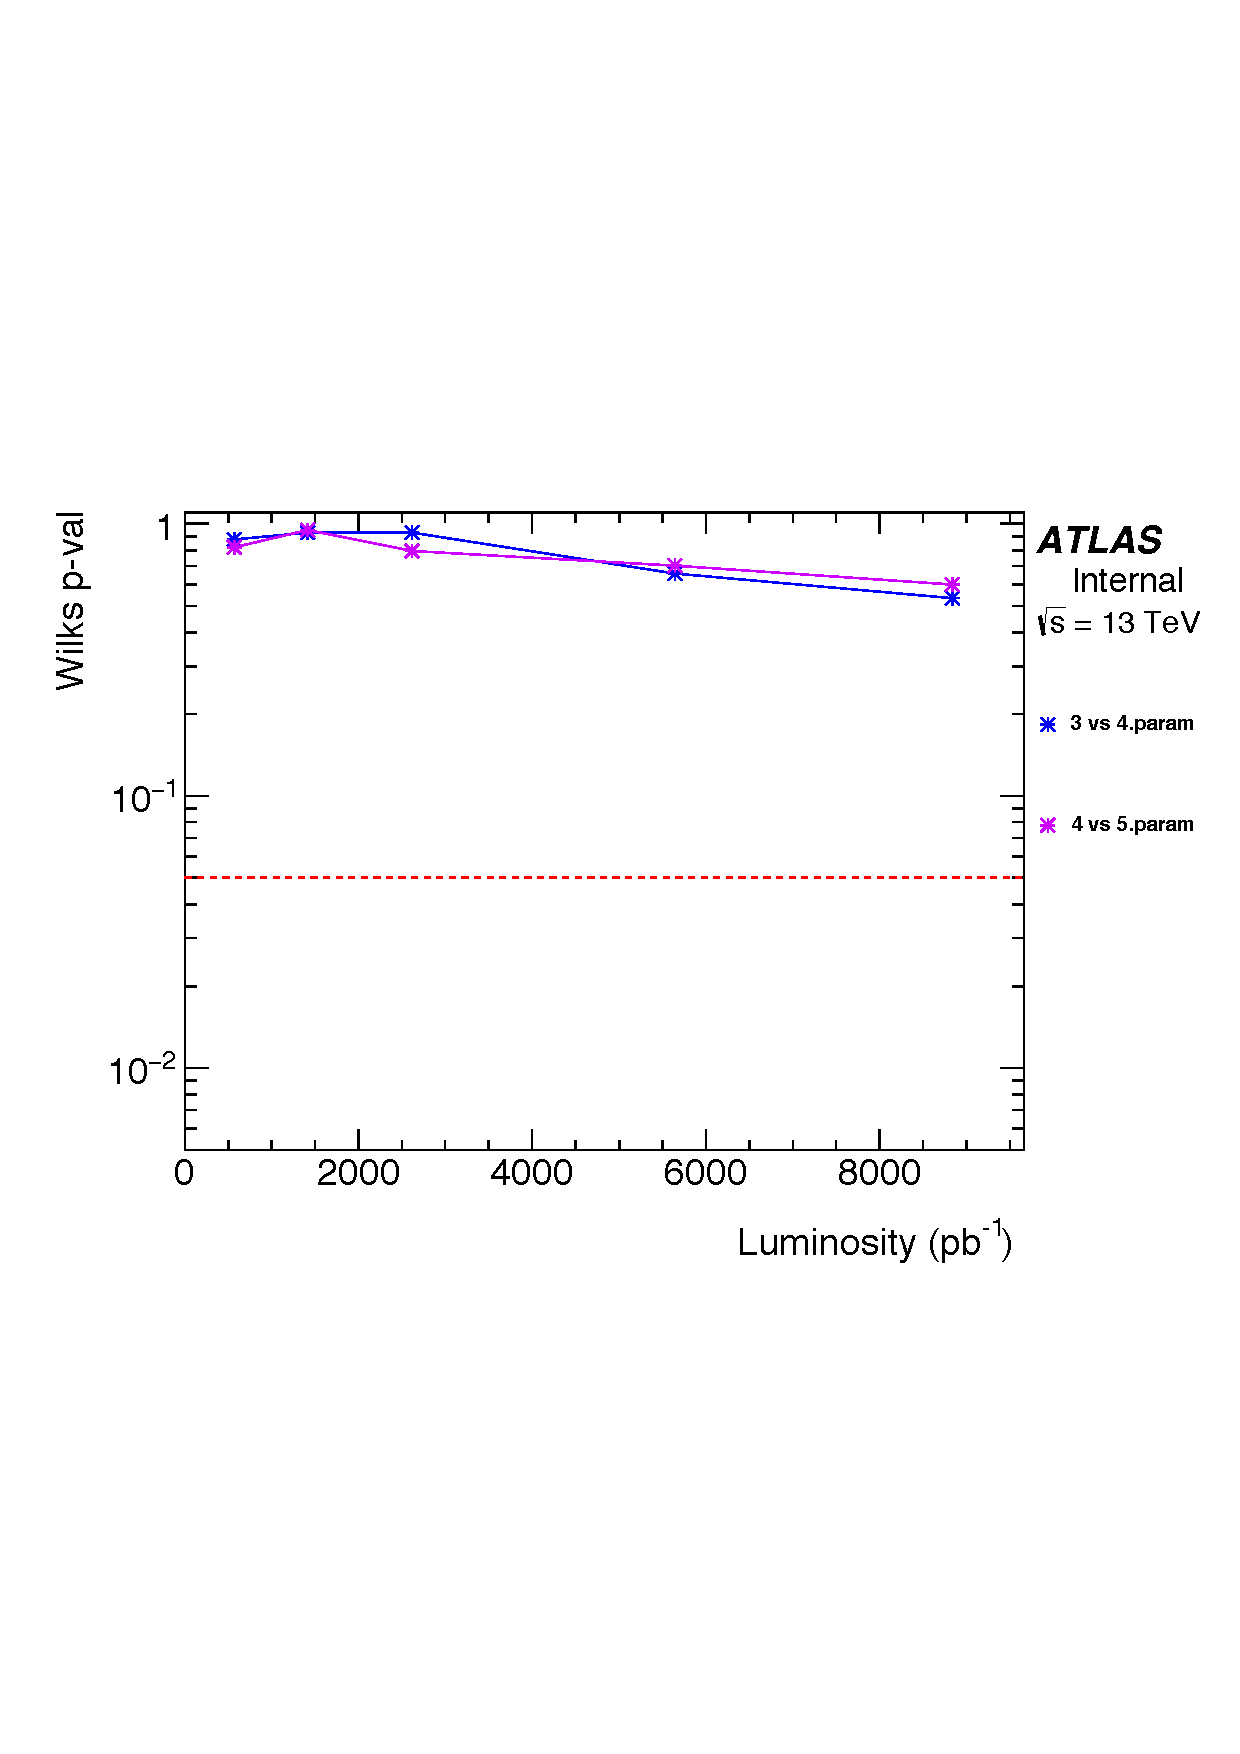
\includegraphics[width=0.47\linewidth, angle=0]{figs/Dibjet/ICHEP/bkg-WilksStat_bb.pdf}}
   \subcaptionbox{$\geq$1 $b$-tag}{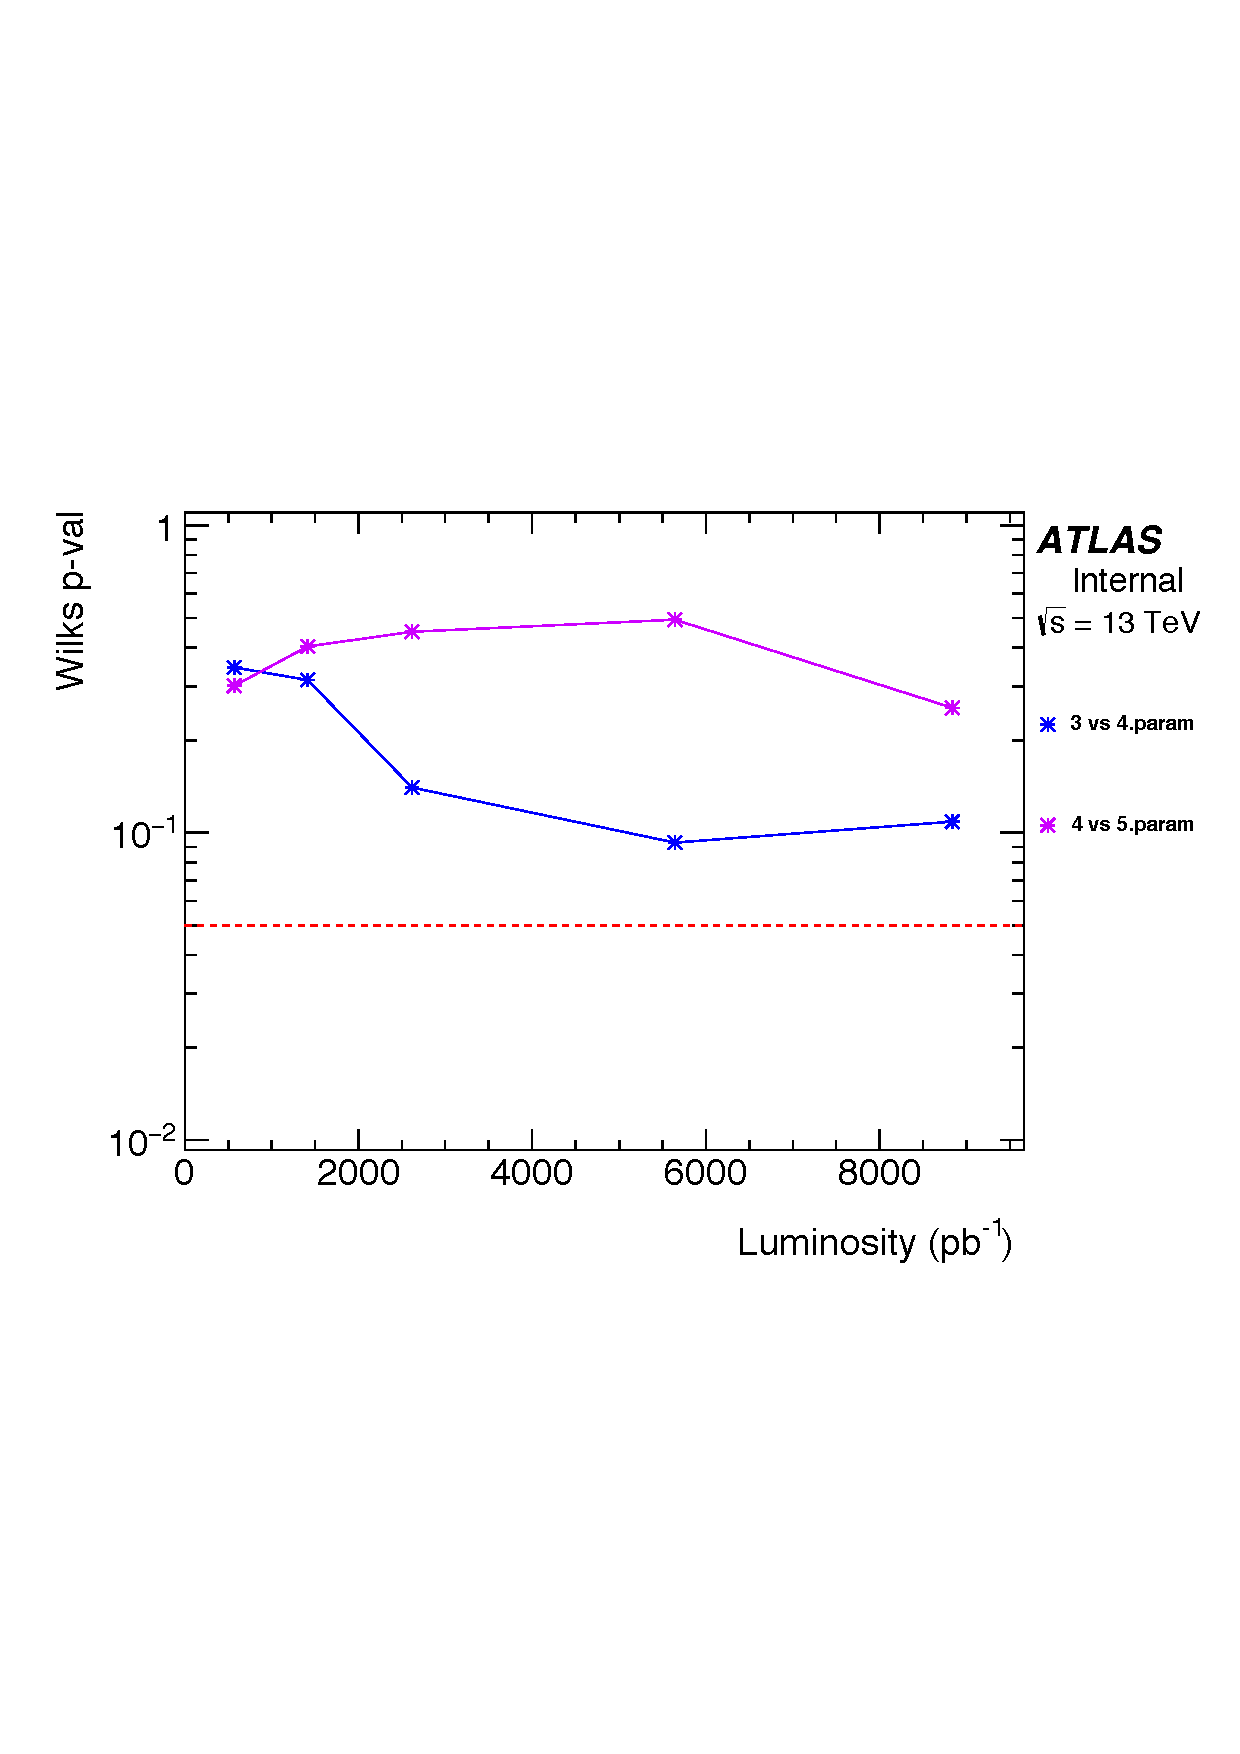
\includegraphics[width=0.47\linewidth, angle=0]{figs/Dibjet/ICHEP/bkg-WilksStat_b.pdf}}
  \end{center}
  
  \caption[The Wilks' \mbox{$p$-value} as a function of luminosity
    in the case that the 3 parameter is the nominal function and the 4 parameter is the alternate (blue)
    and the case where the 4 parameter is the nominal function and the 5 parameter is the alternate (purple)
    for a 8.8 \ifb{} subset of data in the (a) 2 $b$-tag and (b) $\geq1$ $b$-tag category.
    The \summer{} data-set event selection has been applied.]
          {The Wilks' \mbox{$p$-value} as a function of luminosity
            in the case that the 3 parameter is the nominal function and the 4 parameter is the alternate (blue)
            and the case where the 4 parameter is the nominal function and the 5 parameter is the alternate (purple)
            for a 8.8 \ifb{} subset of data in the (a) 2 $b$-tag and (b) $\geq1$ $b$-tag category.
            The \summer{} data-set event selection has been applied~\cite{dibjet-ichep_conf}.
  }
  \label{fig:bkg-summer-wilks}
\end{figure}

\subsection{Fit Tests: Background-Only Data-set}
\label{sec:bkg-summer_fitCR}

To demonstrate that the dijet fit functions are a valid description of the background,
fit tests are performed to a representative background-only data-set.

To perform these tests, the simulated QCD dijet sample described in Section~\ref{sec:evt-s+b} is used as the representative background-only data-set.
The simulation sample is produced in several slices of leading jet $p_{T}$, where each slice contains the same number of events.
A weight is applied to each event such that the final distribution is representative of the smoothly falling dijet mass spectrum that is expected,
whilst still maintaining a similar precision across the full mass range.
The weighted dijet mass distribution is then scaled to 10 \ifb{} \footnote{
  These studies were carried out during data-taking
  and as such the final integrated luminosity of the data-set had to be estimated,
  10 \ifb{} was used where the final data-set is 13.3 \ifb{}.
},
this is referred to as the  `scaled distribution', which can be interpreted as the expected number of data events in a specific mass bin. 
The precision of the scaled distribution is represented by the number of `effective entries';
the number of effective entries is the number of data events that would be required to give the same precision,
or to put it another way it is the square of the error in that mass bin. The number of effective entries can be calculated from the event weights as shown in Equation~\ref{eq:effEnt}.
\begin{equation}
  N_{eff} = (\sum{w_i})^2 / \sum{w_i^2}
  \label{eq:effEnt}
\end{equation}
Figure~\ref{fig:effEnt} shows the scaled and effective entries distributions as a function of dijet mass for the 2 $b$-tag and $\geq$1 $b$-tag categories.
The oscillating pattern in the effective entry distribution is cause by the merging of the different jet-\pT{} slices of the simulated sample. 

\begin{figure}[!ht]
  \begin{center}
    \captionsetup[subfigure]{aboveskip=0pt,justification=centering}
   \subcaptionbox{2 $b$-tag}{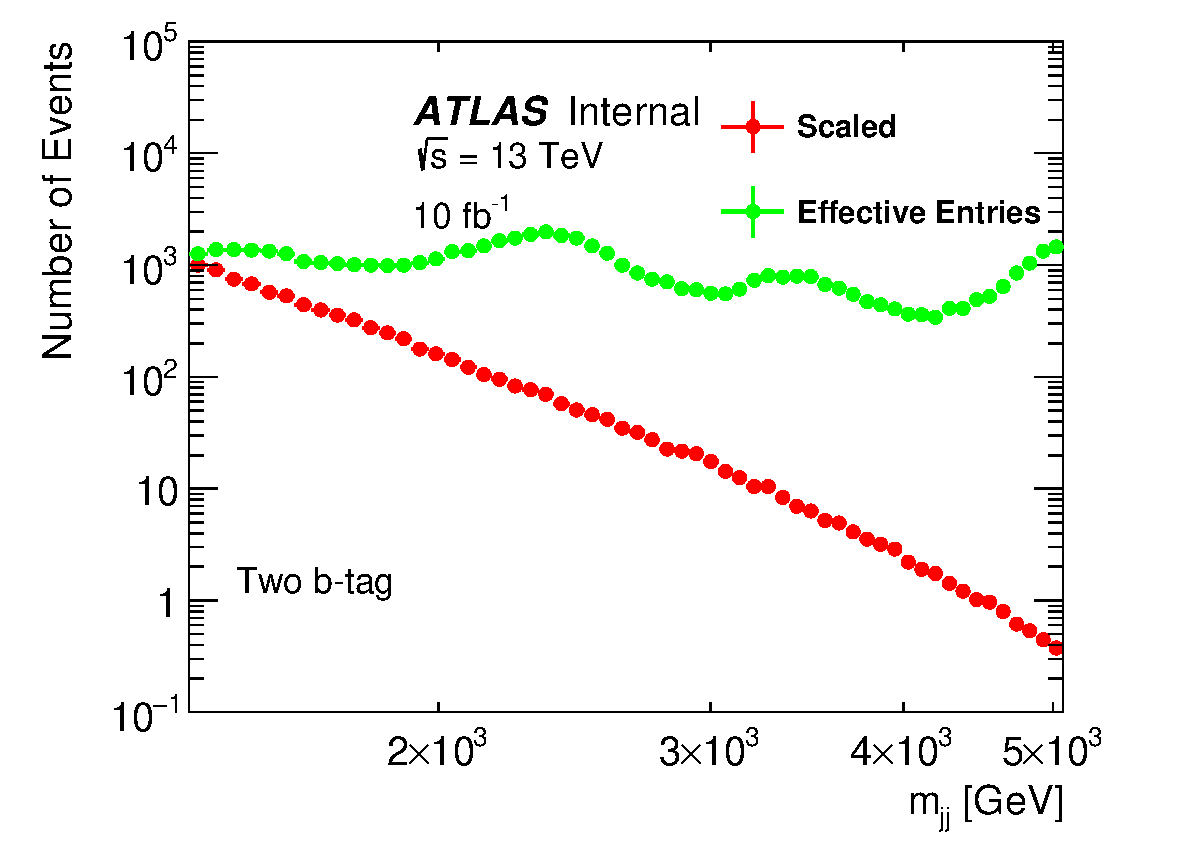
\includegraphics[width=0.47\linewidth, angle=0]{figs/Dibjet/ICHEP/FitRange/mbb_fix_8585_effEntries_Logx_10fb.pdf}}
   \subcaptionbox{$\geq$1 $b$-tag}{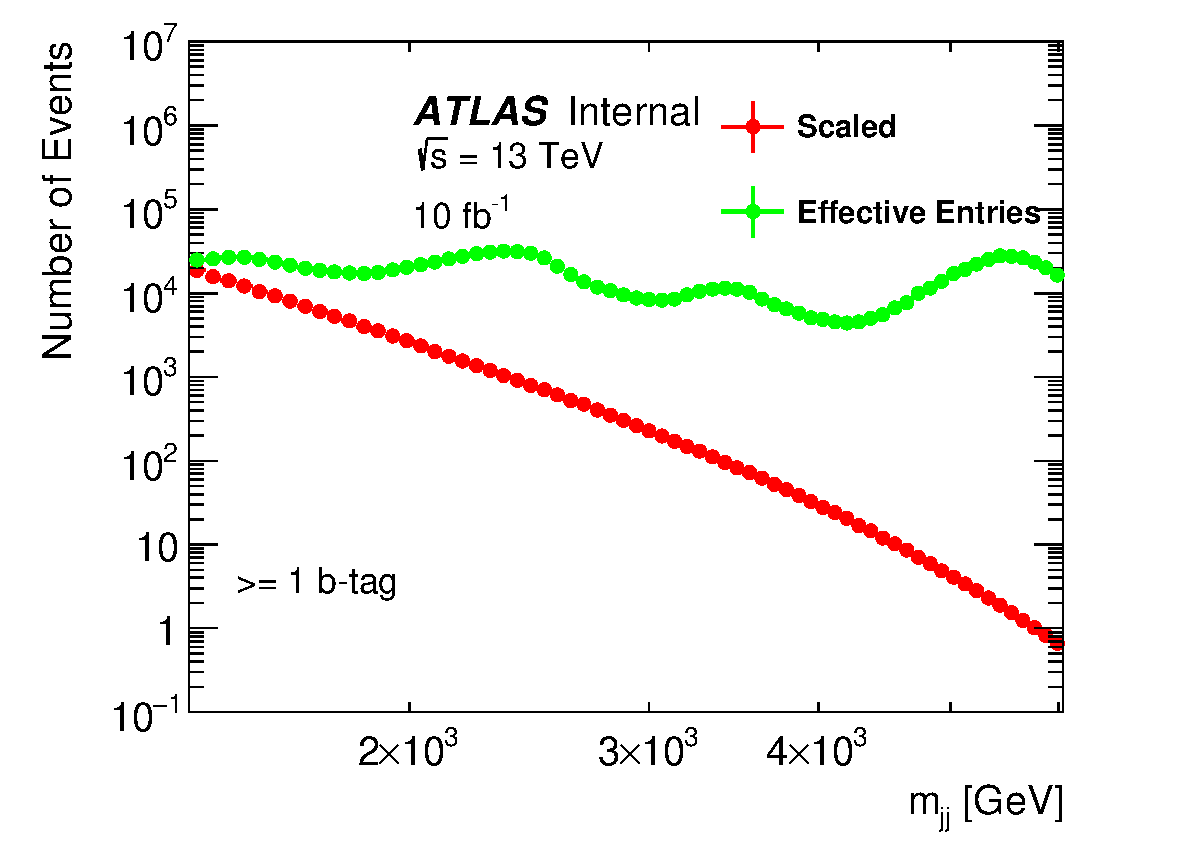
\includegraphics[width=0.47\linewidth, angle=0]{figs/Dibjet/ICHEP/FitRange/mbj_inc_fix_8585_effEntries_Logx_10fb.pdf}}
  \end{center}
  \caption{The scaled dijet mass distribution (red) compared to the
    effective entries dijet mass distribution (green)
    of Monte-Carlo simulation for the (a) 2 $b$-tag and (b) $\geq$1 $b$-tag category.
    The \summer{} data-set event selection has been applied.}
  \label{fig:effEnt}
\end{figure}

\subsection{Fit Tests: Mass Range Studies}
\label{sec:bkg-summer_range}

To demonstrate that the dijet fit functions are able to describe the dijet mass spectra in the mass range considered,
the search phase is applied to the scaled dijet mass spectra from simulation.
The errors on the dijet mass spectrum are given by the square root of the number of effective entries
which effectively gives the statistical error of the simulated sample.

The initial dijet mass spectra considered have a lower mass edge of $m_{jj}$ = 1100 GeV,
selected such that there is no kinematic bias from the single jet trigger,
and an upper mass edge at the \mjj{} bin at which the dijet mass spectrum goes below one entry.
Figure~\ref{fig:Short_4para_1100_figure1} and \ref{fig:Short_5para_1100_figure1} show the search phase
for both $b$-tag categories, using the 4 and 5 parameter dijet fit functions respectively.
The most discrepant excess is indicated by the blue lines and the \bh{} \mbox{$p$-value} of the excess is shown on the plot,
which has been calculated using 10,000 pseudo-experiments.
Similarly, the \mbox{$p$-value} of the most discrepant deficit is calculated using the same process, which is referred to as \dhunt{},
and an overall quality of fit \mbox{$p$-value} is also calculated by the same process using the $\chi^{2}$ test statistic.
The lower panel shows the significance in each~\mjj{} bin,
defined as the difference between the data and the background estimate divided by the error on the data point.

For both fit functions in the $\geq$1 $b$-tag category,
a large excess is observed which has been assigned a \bh{} \mbox{$p$-value} of $<$0.0001
\footnote{This means that the observed \bh{} test-statistic was greater than in all 10,000 pseudo-experiments.}.
This shows that the 4 and 5 parameter dijet fit functions provide a poor description
of the background distribution from simulation in the $\geq1$ $b$-tag category.
It can also be concluded that the 3 parameter dijet fit function will also be inadequate, as it is a subset of the 4 parameter dijet fit function.

\begin{figure}[!ht]
  \begin{center}
   \captionsetup[subfigure]{aboveskip=0pt,justification=centering}
   \subcaptionbox{2 $b$-tag}{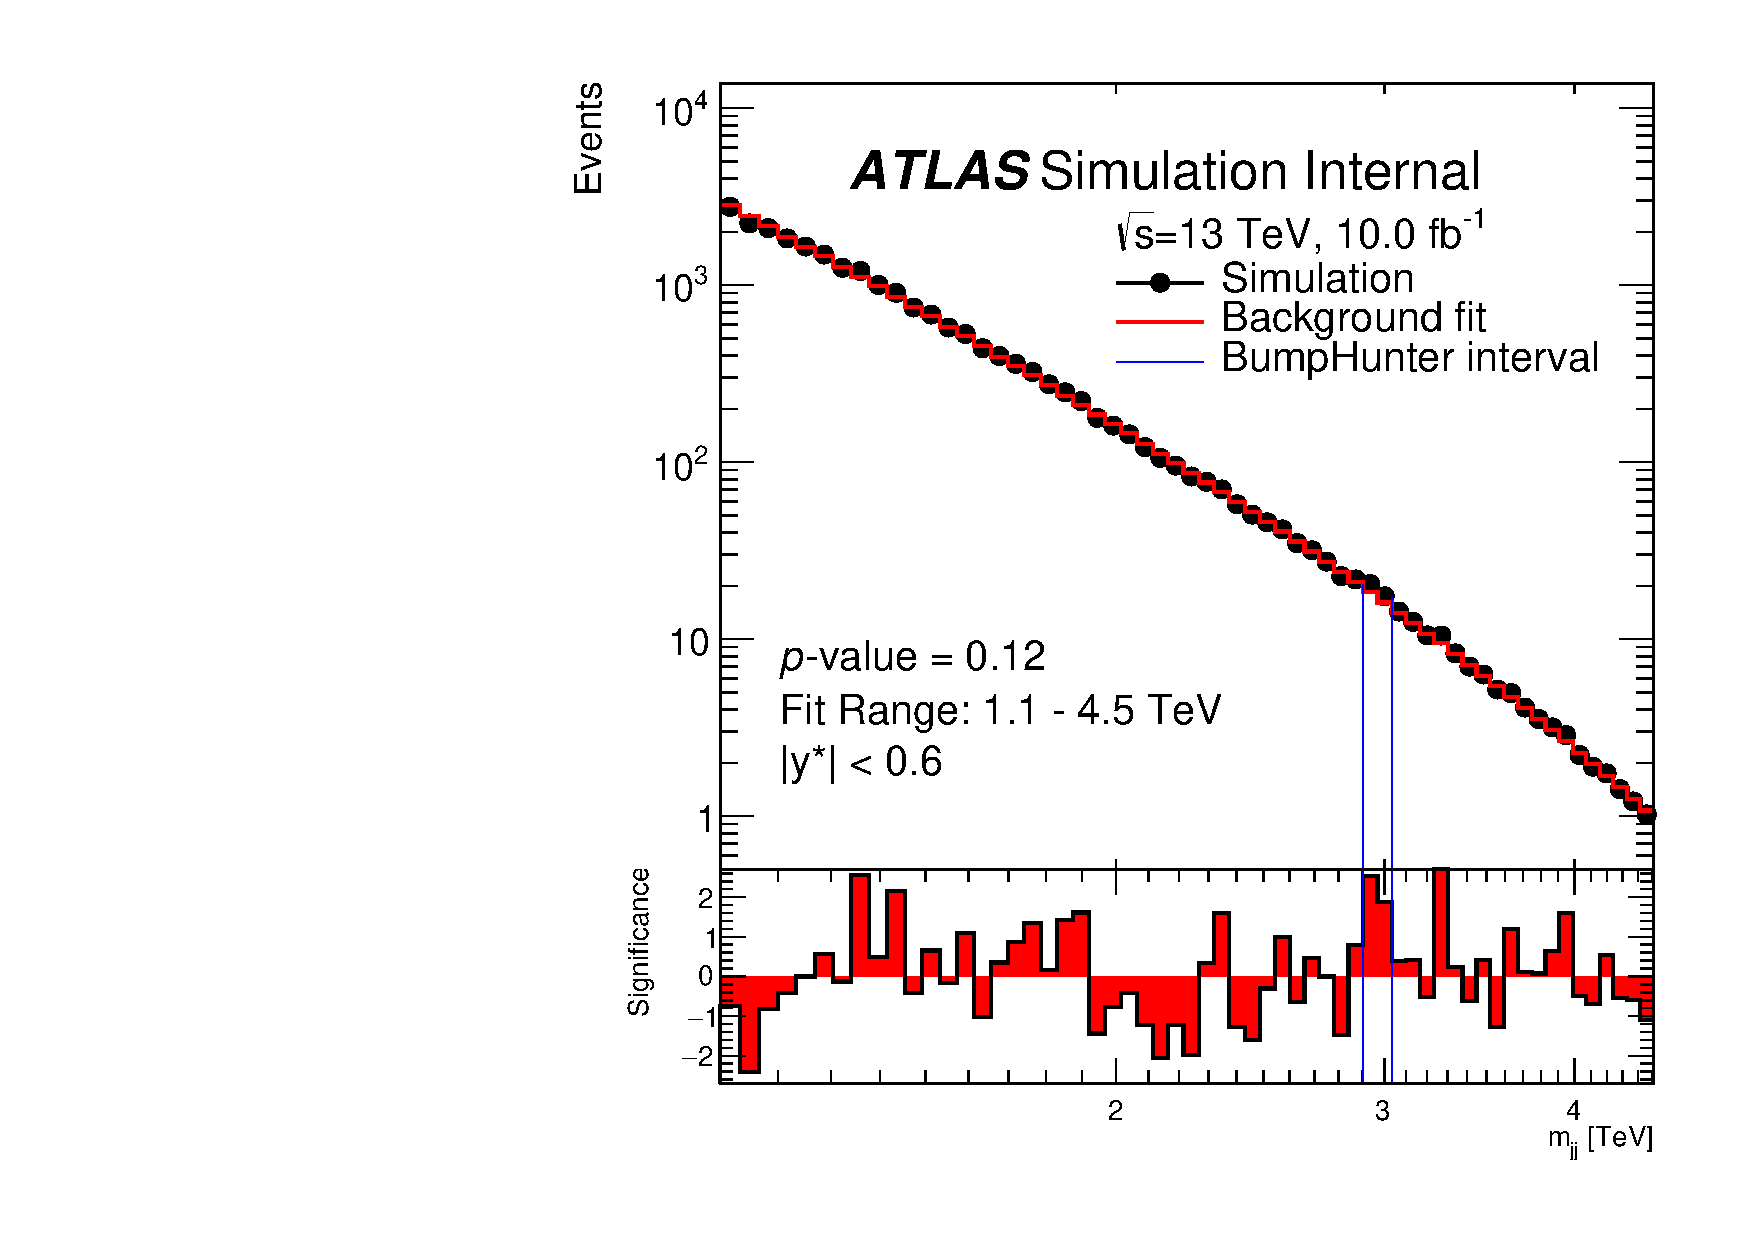
\includegraphics[width=0.47\linewidth, angle=0]{figs/Dibjet/ICHEP/FitRange/mbb_fix_8585_Short_4para_1100_figure1_10fb.pdf}}
   \subcaptionbox{$\geq$1 $b$-tag}{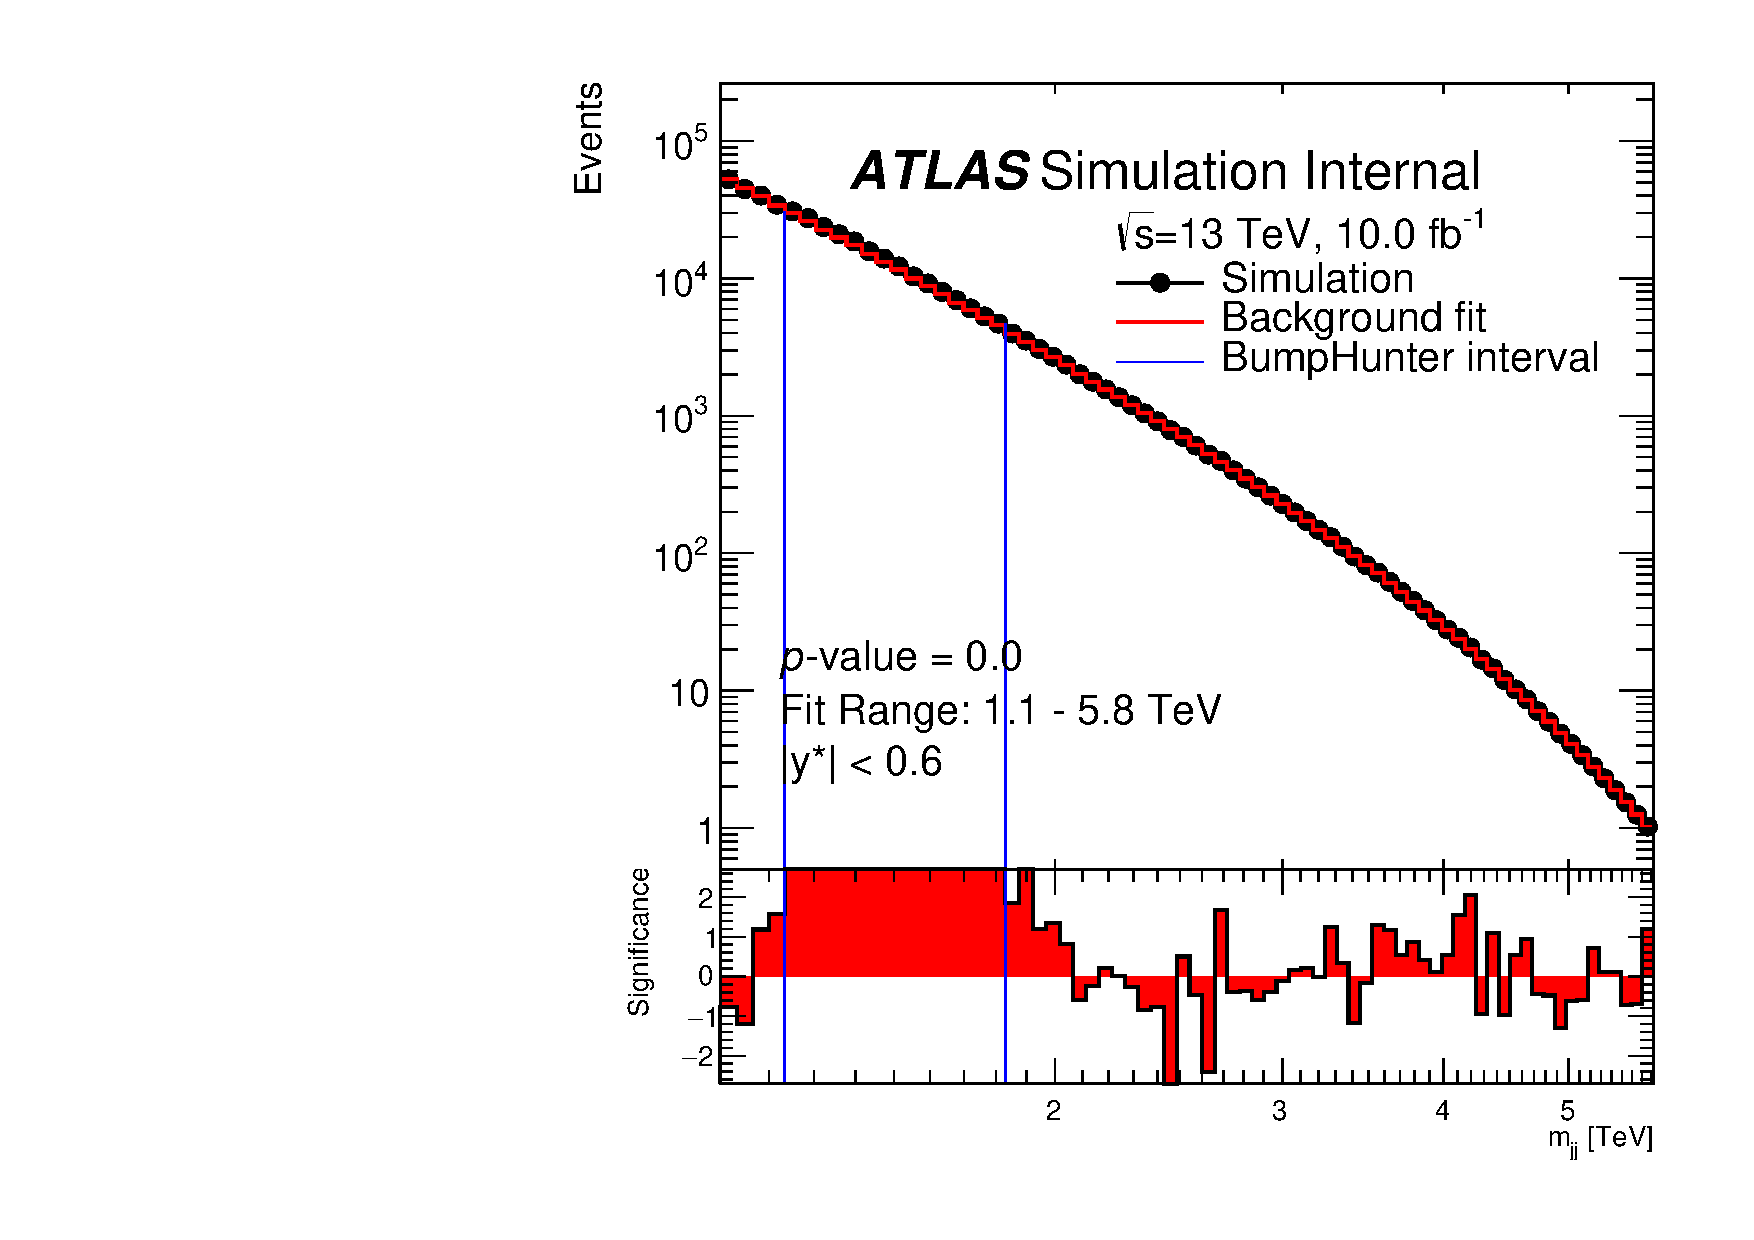
\includegraphics[width=0.47\linewidth, angle=0]{figs/Dibjet/ICHEP/FitRange/mbj_inc_fix_8585_Short_4para_1100_figure1_10fb.pdf}}
  \end{center}
  \caption{ The dijet mass distribution taken from multi-jet simulation for the (a) 2 $b$-tag and (b) $\geq$1 $b$-tag,
   category, fitted to using the 4 parameter fit function, with lower mass bound of the fit range $m_{jj}$ = 1100 GeV.
   The \bh{} algorithm is run to identify the most discrepant excess, as indicated by the blue lines.
   Pseudo-experiments are used to assign the excess a \mbox{$p$-value}, which is shown on the plot.    
   The \summer{} data-set event selection has been applied.}
 \label{fig:Short_4para_1100_figure1}
\end{figure}


\begin{figure}[!ht]
  \begin{center}
    \captionsetup[subfigure]{aboveskip=0pt,justification=centering}
   \subcaptionbox{2 $b$-tag}{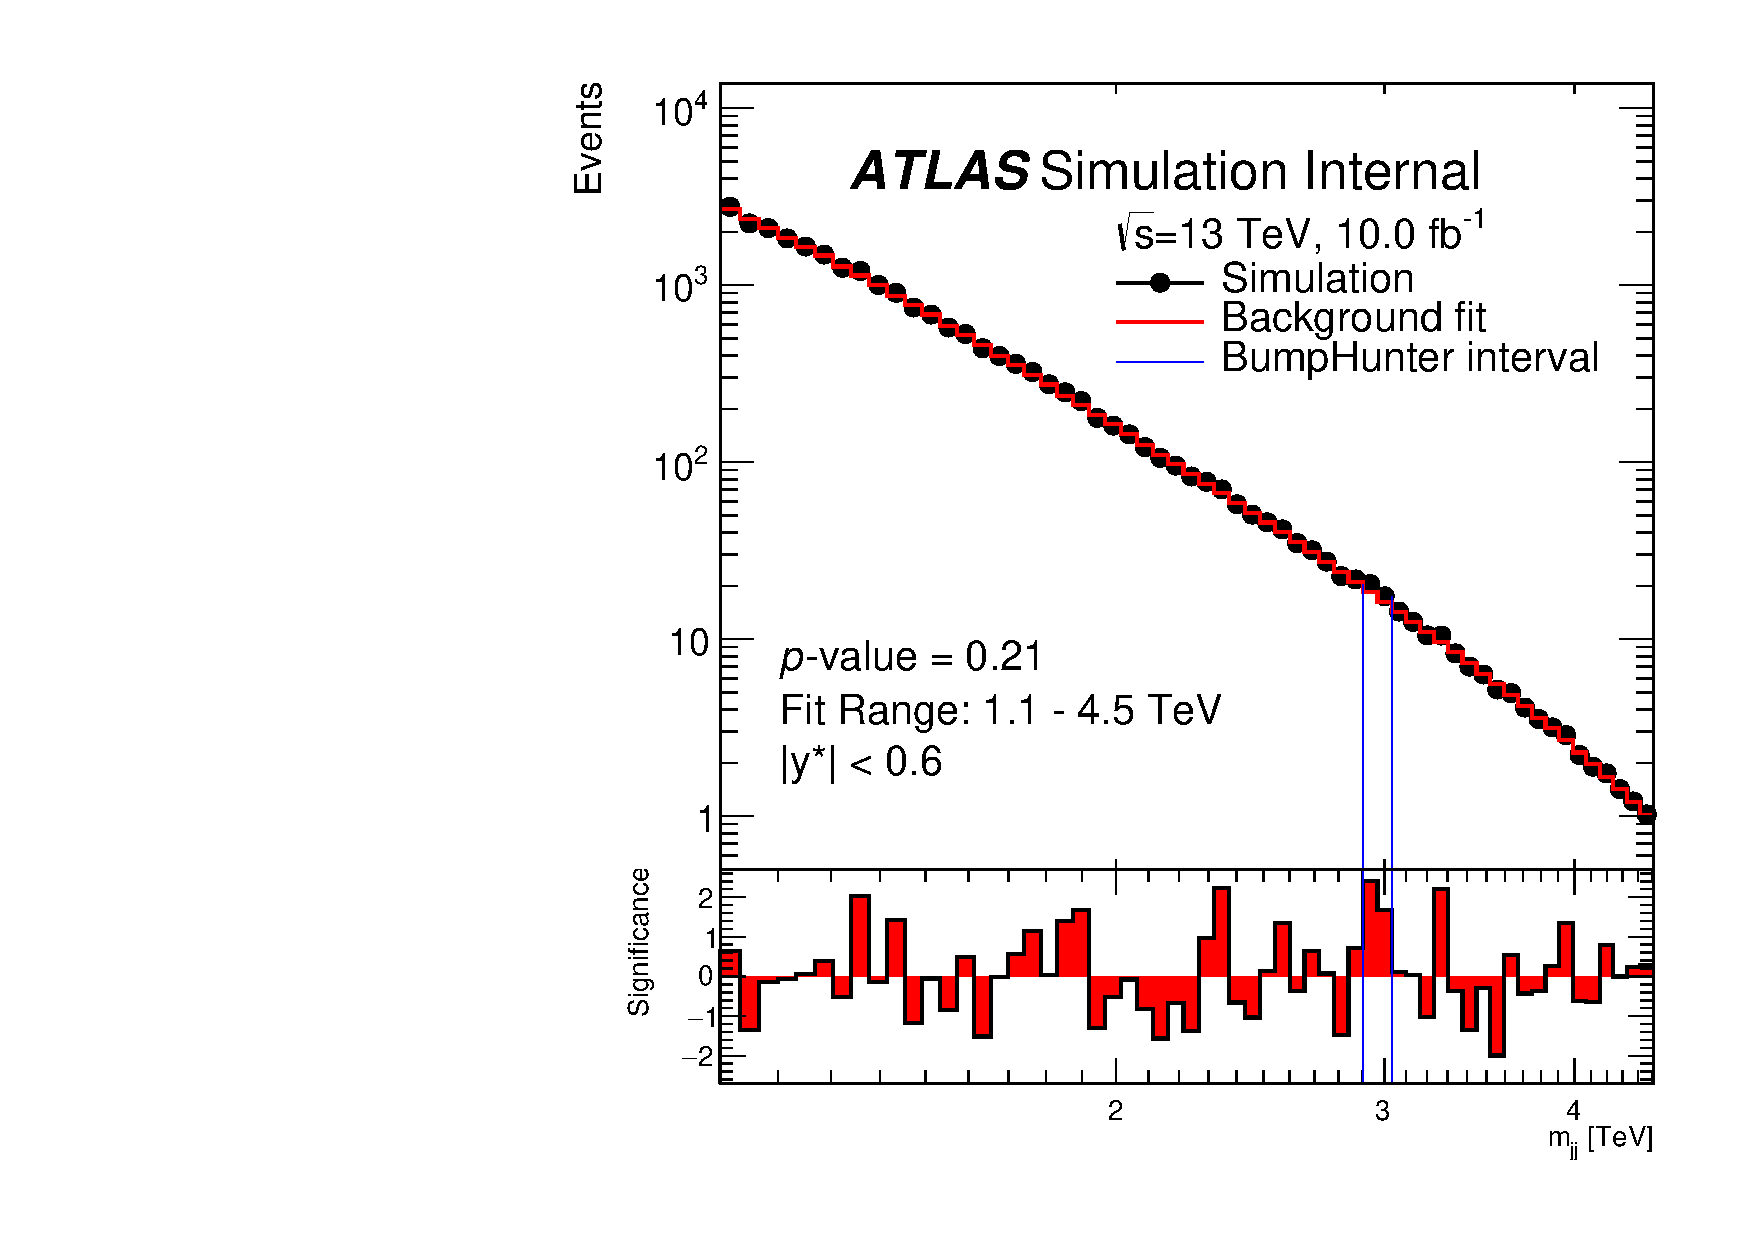
\includegraphics[width=0.47\linewidth, angle=0]{figs/Dibjet/ICHEP/FitRange/mbb_fix_8585_Short_5para_1100_figure1_10fb.pdf}}
   \subcaptionbox{$\geq$1 $b$-tag}{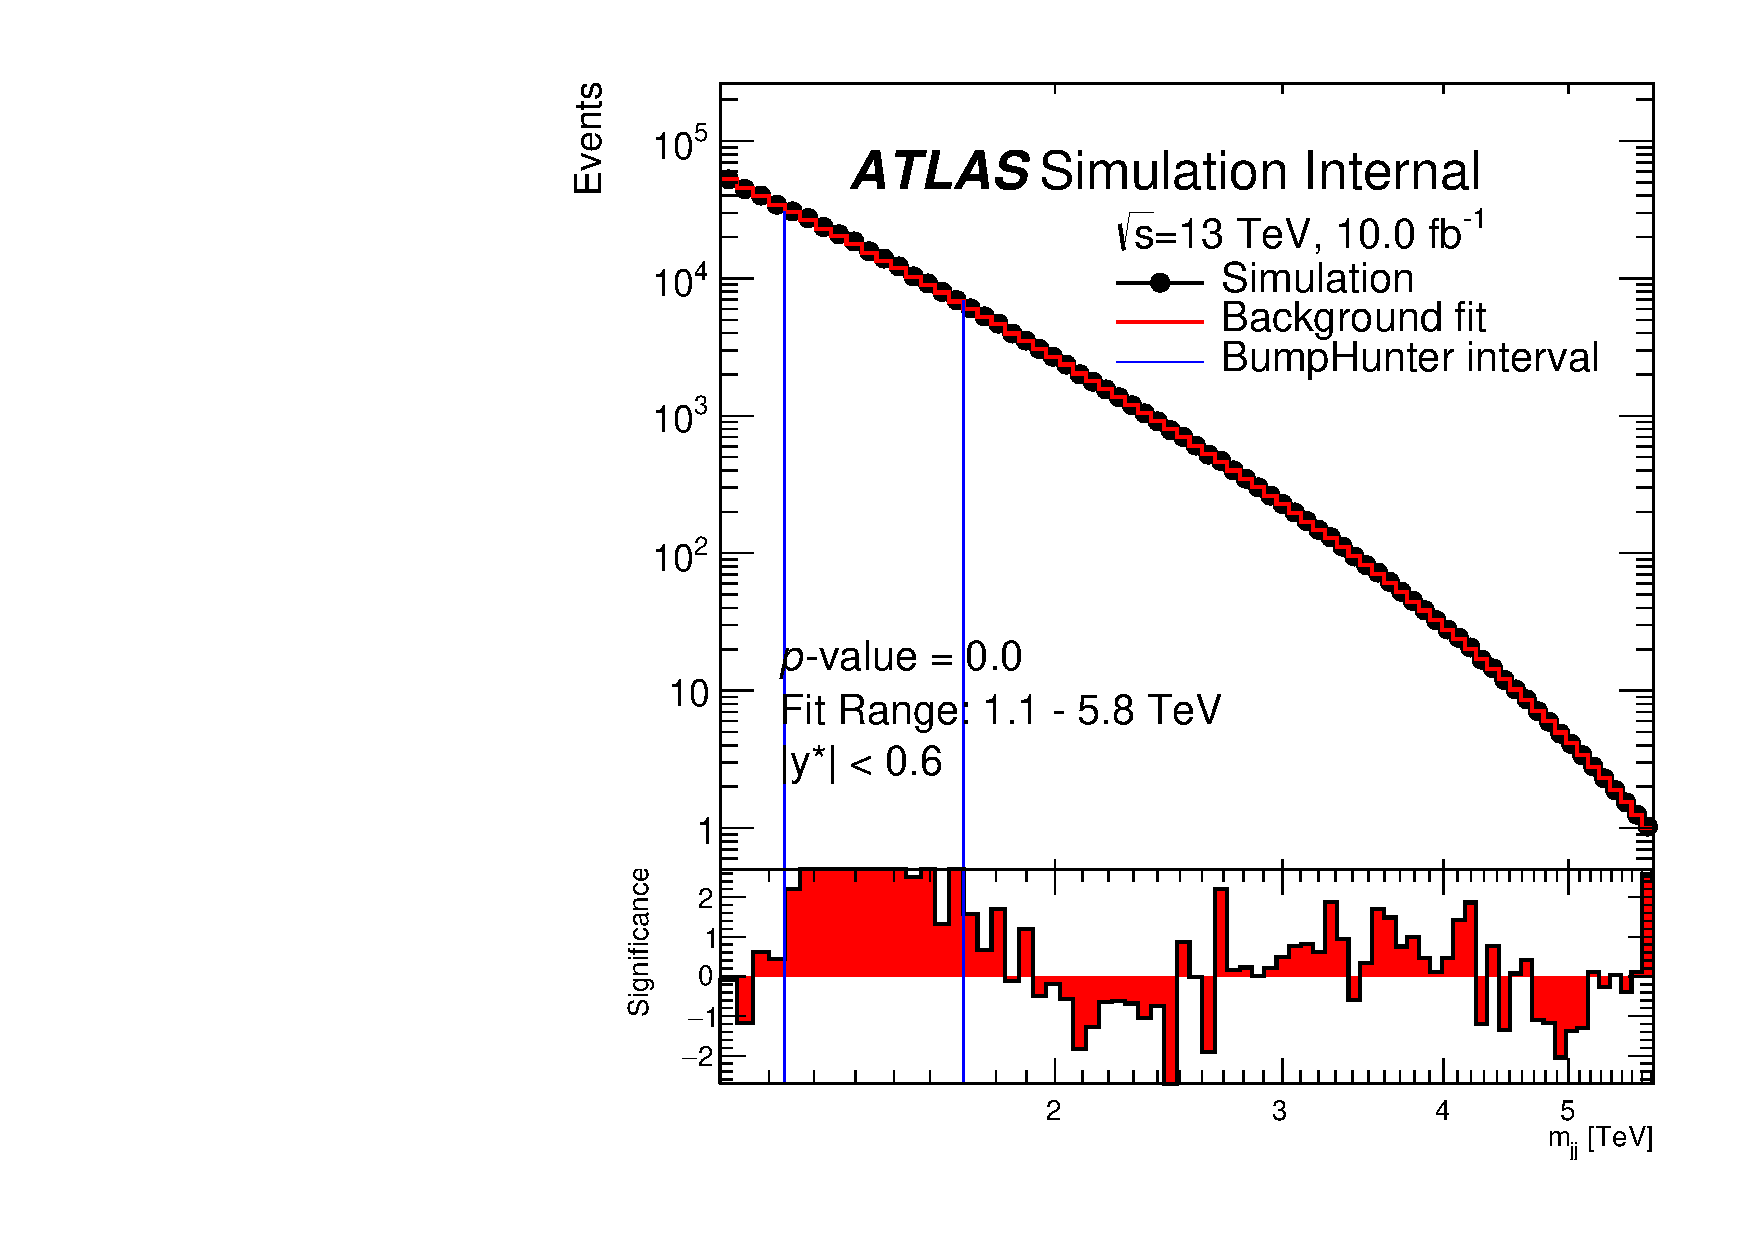
\includegraphics[width=0.47\linewidth, angle=0]{figs/Dibjet/ICHEP/FitRange/mbj_inc_fix_8585_Short_5para_1100_figure1_10fb.pdf}}
  \end{center}
  \caption{ The dijet mass distribution taken from multi-jet simulation for the (a) 2 $b$-tag and (b) $\geq$1 $b$-tag,
    category, fitted to using the 5 parameter fit function, with lower mass bound of the fit range $m_{jj}$ = 1100 GeV.
    The \bh{} algorithm is run to identify the most discrepant excess, as indicated by the blue lines.
    Pseudo-experiments are used to assign the excess a \mbox{$p$-value}, which is shown on the plot.
    The \summer{} data-set event selection has been applied.}
  \label{fig:Short_5para_1100_figure1}
\end{figure}

\FloatBarrier

However, by changing the lower mass bound of the fit,
a region can be found where the dijet fit functions are able to describe the background accurately.
To find the largest region with a stable fit quality, the simulated dijet mass spectrum is
fitted to using the 4 parameter dijet fit function with the lower mass bound of the fit region increased one bin at a time,
beginning at $m_{jj}$ = 1100 GeV up to $m_{jj}$ = 1500 GeV.
As before the upper edge of the fit region is the mass bin at which the simulation goes below one entry per bin.
Figure~\ref{fig:mjjGraphs_bb} and \ref{fig:mjjGraphs_bj_inc} show,
for the 2 $b$-tag and $\geq1$ $b$-tag categories, the distributions of the
(a) \bh{}, (b) \dhunt{} and (c) $\chi^{2}$ \mbox{$p$-value}s as the lower mass bound of the fit region is increased.
In both categories it is shown that there are fit regions that are stable if the lower mass bound is $m_{jj}$ = 1378 GeV or above.
This demonstrates that there are features in the background mass spectrum at low masses that are causing a poor fit quality,
which can be removed by using a fit region $m_{jj} >$ 1378 GeV. 

Figure~\ref{fig:Short_4para_1378_figure1} shows the search phase applied to the dijet mass spectra
of the simulated sample for both $b$-tagging categories,
for the fit range with the lower mass bound of $m_{jj}$ = 1378 GeV,
fitted to using the 4 parameter fit function.
The most discrepant excess, as found by the \bh{} algorithm, is indicated by the blue lines
and the \mbox{$p$-value} of the excess is shown on the plot.
This shows that the fit quality is reasonable for this choice of fit region.
The study presented in this section motivates the choice of $m_{jj} >$ 1378 GeV
as the lower mass cut used in the \summer{} data-set event selection.

\begin{figure}[!htb]
  \begin{center}
    \captionsetup[subfigure]{aboveskip=0pt,justification=centering}
    \subcaptionbox{\bh{}}{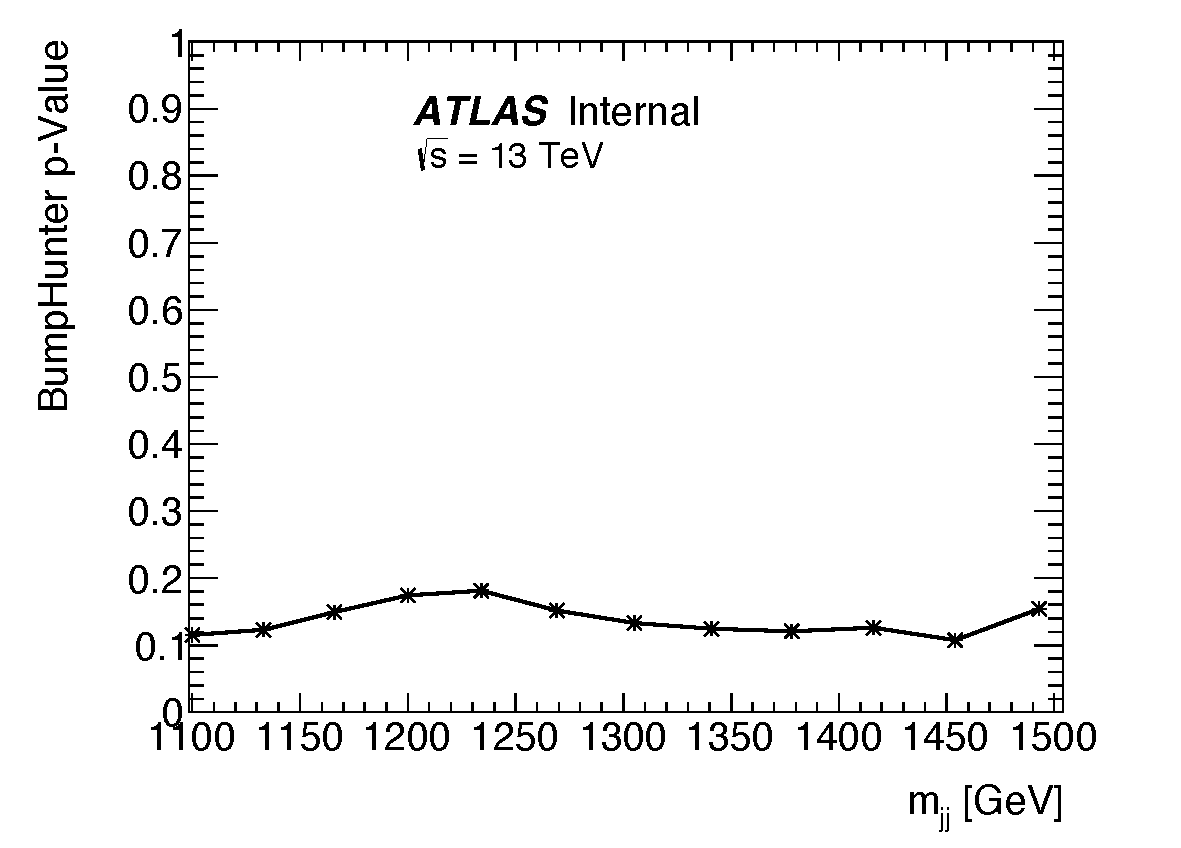
\includegraphics[width=0.4\linewidth, angle=0]{figs/Dibjet/ICHEP/FitRange/mbb_fix_8585_mjjGraph_bumpHunter_10fb.pdf}}
    \subcaptionbox{\dhunt{}}{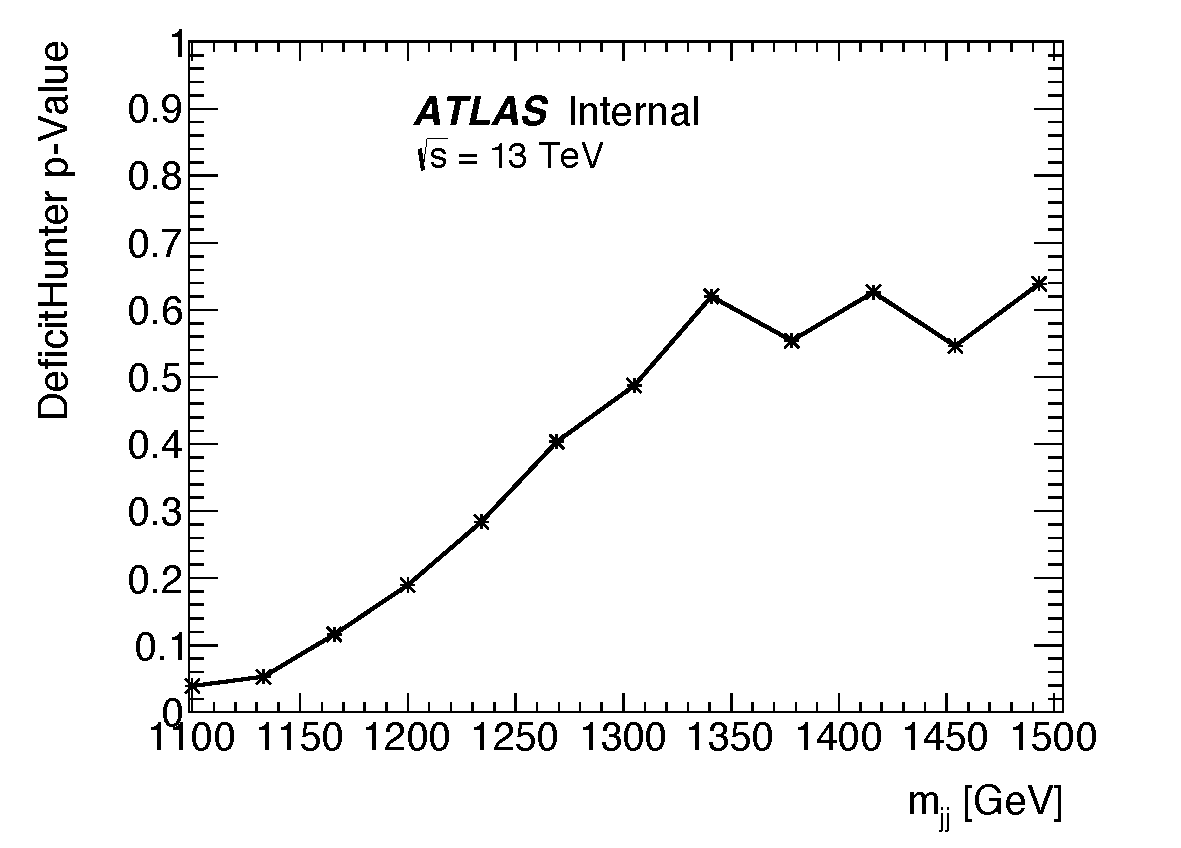
\includegraphics[width=0.4\linewidth, angle=0]{figs/Dibjet/ICHEP/FitRange/mbb_fix_8585_mjjGraph_deficitOnlyHunter_10fb.pdf}}\\
    \subcaptionbox{$\chi^{2}$}{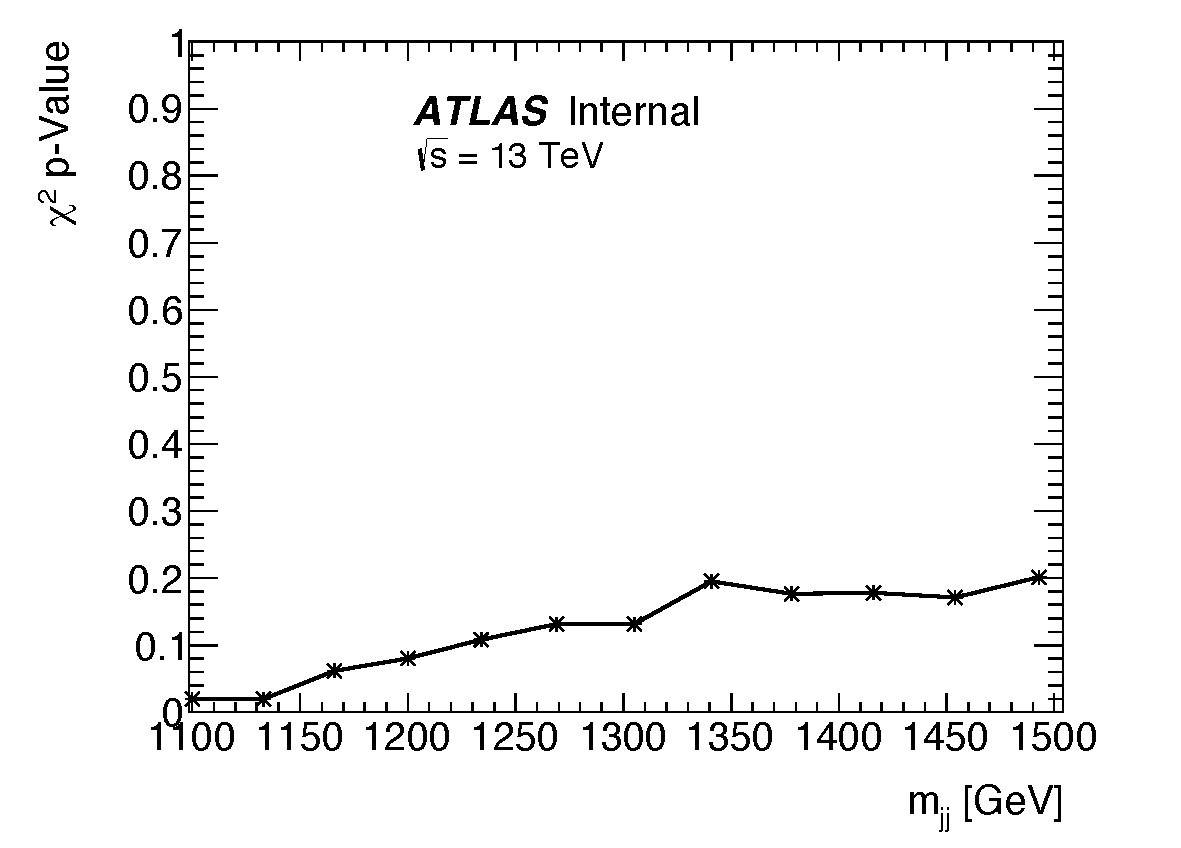
\includegraphics[width=0.4\linewidth, angle=0]{figs/Dibjet/ICHEP/FitRange/mbb_fix_8585_mjjGraph_chi2_10fb.pdf}}
  \end{center}
  \caption{The distribution of the (a) \bh{}, (b) \dhunt{} and (c) $\chi^{2}$ \mbox{$p$-value}s
    for different values of lower mass bound of the fit range, when fitting to 2 $b$-tag category
    dijet mass distribution taken from multi-jet simulation with the 4 parameter fit function.
    The \summer{} data-set event selection has been applied, with the exception of the~\mjj{} cut.}
  \label{fig:mjjGraphs_bb}
  \begin{center}
    \captionsetup[subfigure]{aboveskip=0pt,justification=centering}
    \subcaptionbox{\bh{}}{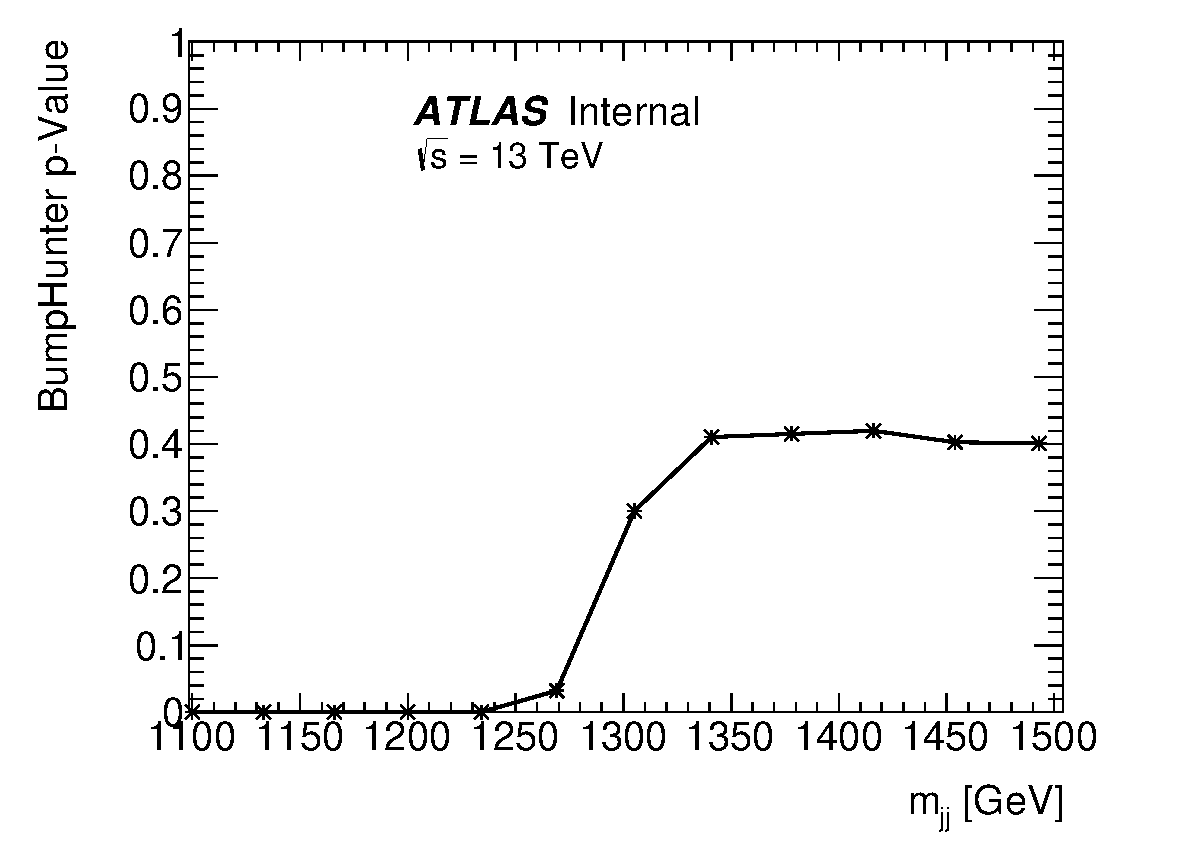
\includegraphics[width=0.4\linewidth, angle=0]{figs/Dibjet/ICHEP/FitRange/mbj_inc_fix_8585_mjjGraph_bumpHunter_10fb.pdf}}
    \subcaptionbox{\dhunt{}}{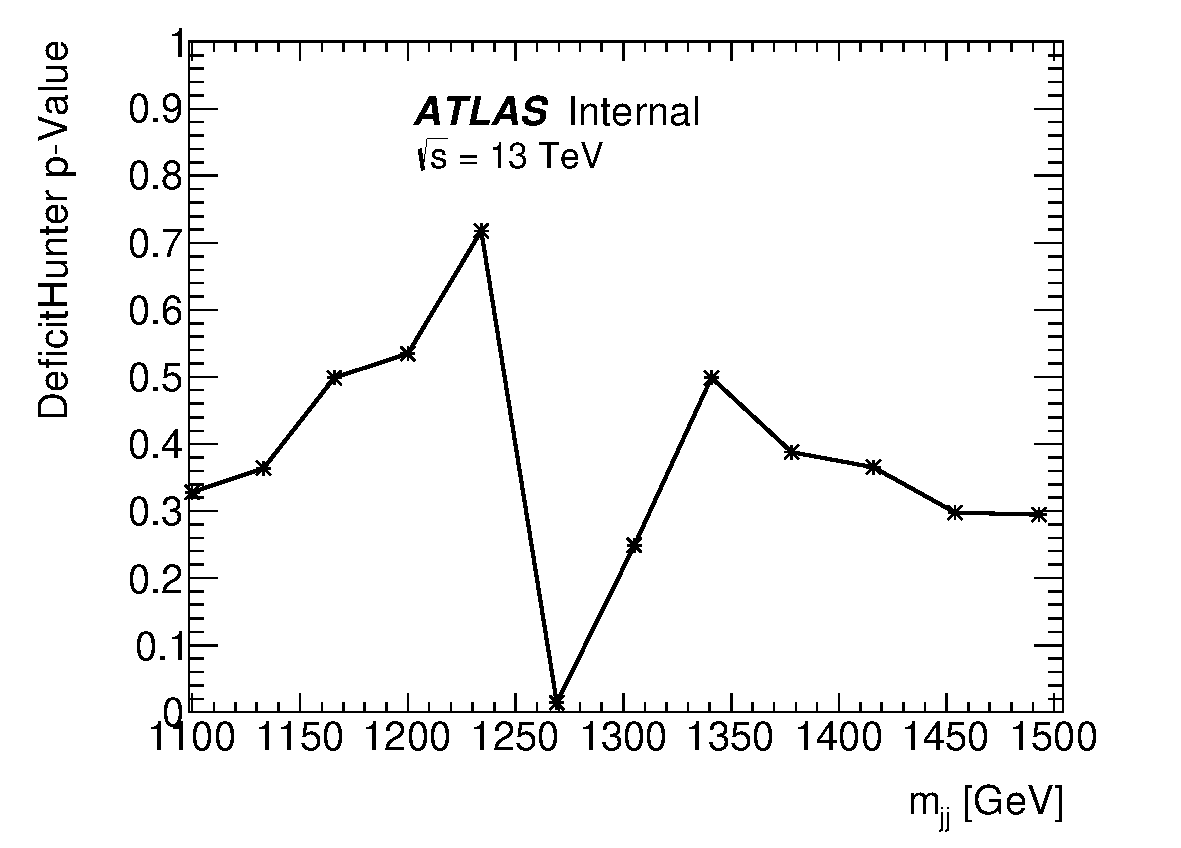
\includegraphics[width=0.4\linewidth, angle=0]{figs/Dibjet/ICHEP/FitRange/mbj_inc_fix_8585_mjjGraph_deficitOnlyHunter_10fb.pdf}}\\
    \subcaptionbox{$\chi^{2}$}{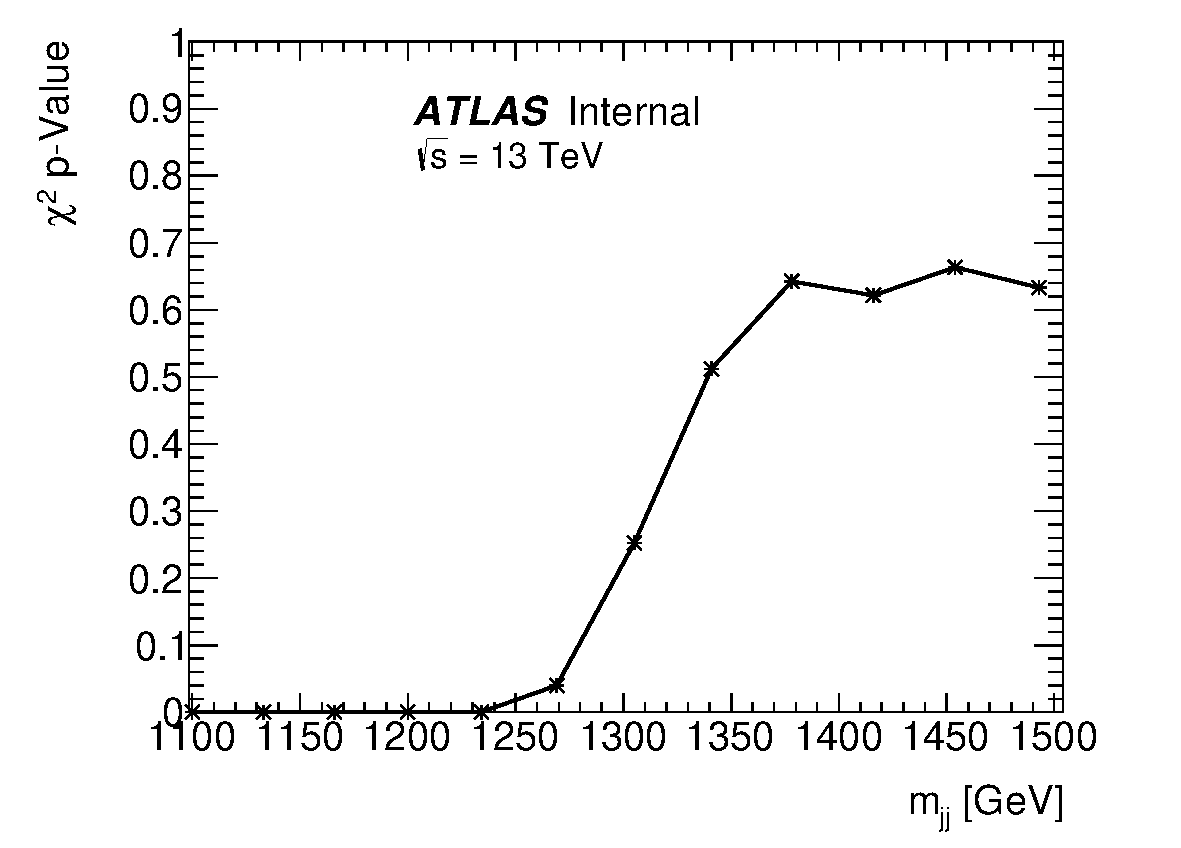
\includegraphics[width=0.4\linewidth, angle=0]{figs/Dibjet/ICHEP/FitRange/mbj_inc_fix_8585_mjjGraph_chi2_10fb.pdf}}
  \end{center}
  \caption{The distribution of the (a) \bh{}, (b) \dhunt{} and (c) $\chi^{2}$ \mbox{$p$-value}s
    for different values of lower mass bound of the fit range, when fitting to $\geq$1 $b$-tag category
    dijet mass distribution taken from multi-jet simulation with the 4 parameter fit function.
    The \summer{} data-set event selection has been applied, with the exception of the~\mjj{} cut.}
  \label{fig:mjjGraphs_bj_inc}
\end{figure}

\begin{figure}[!ht]
  \begin{center}
    \captionsetup[subfigure]{aboveskip=0pt,justification=centering}
   \subcaptionbox{2 $b$-tag}{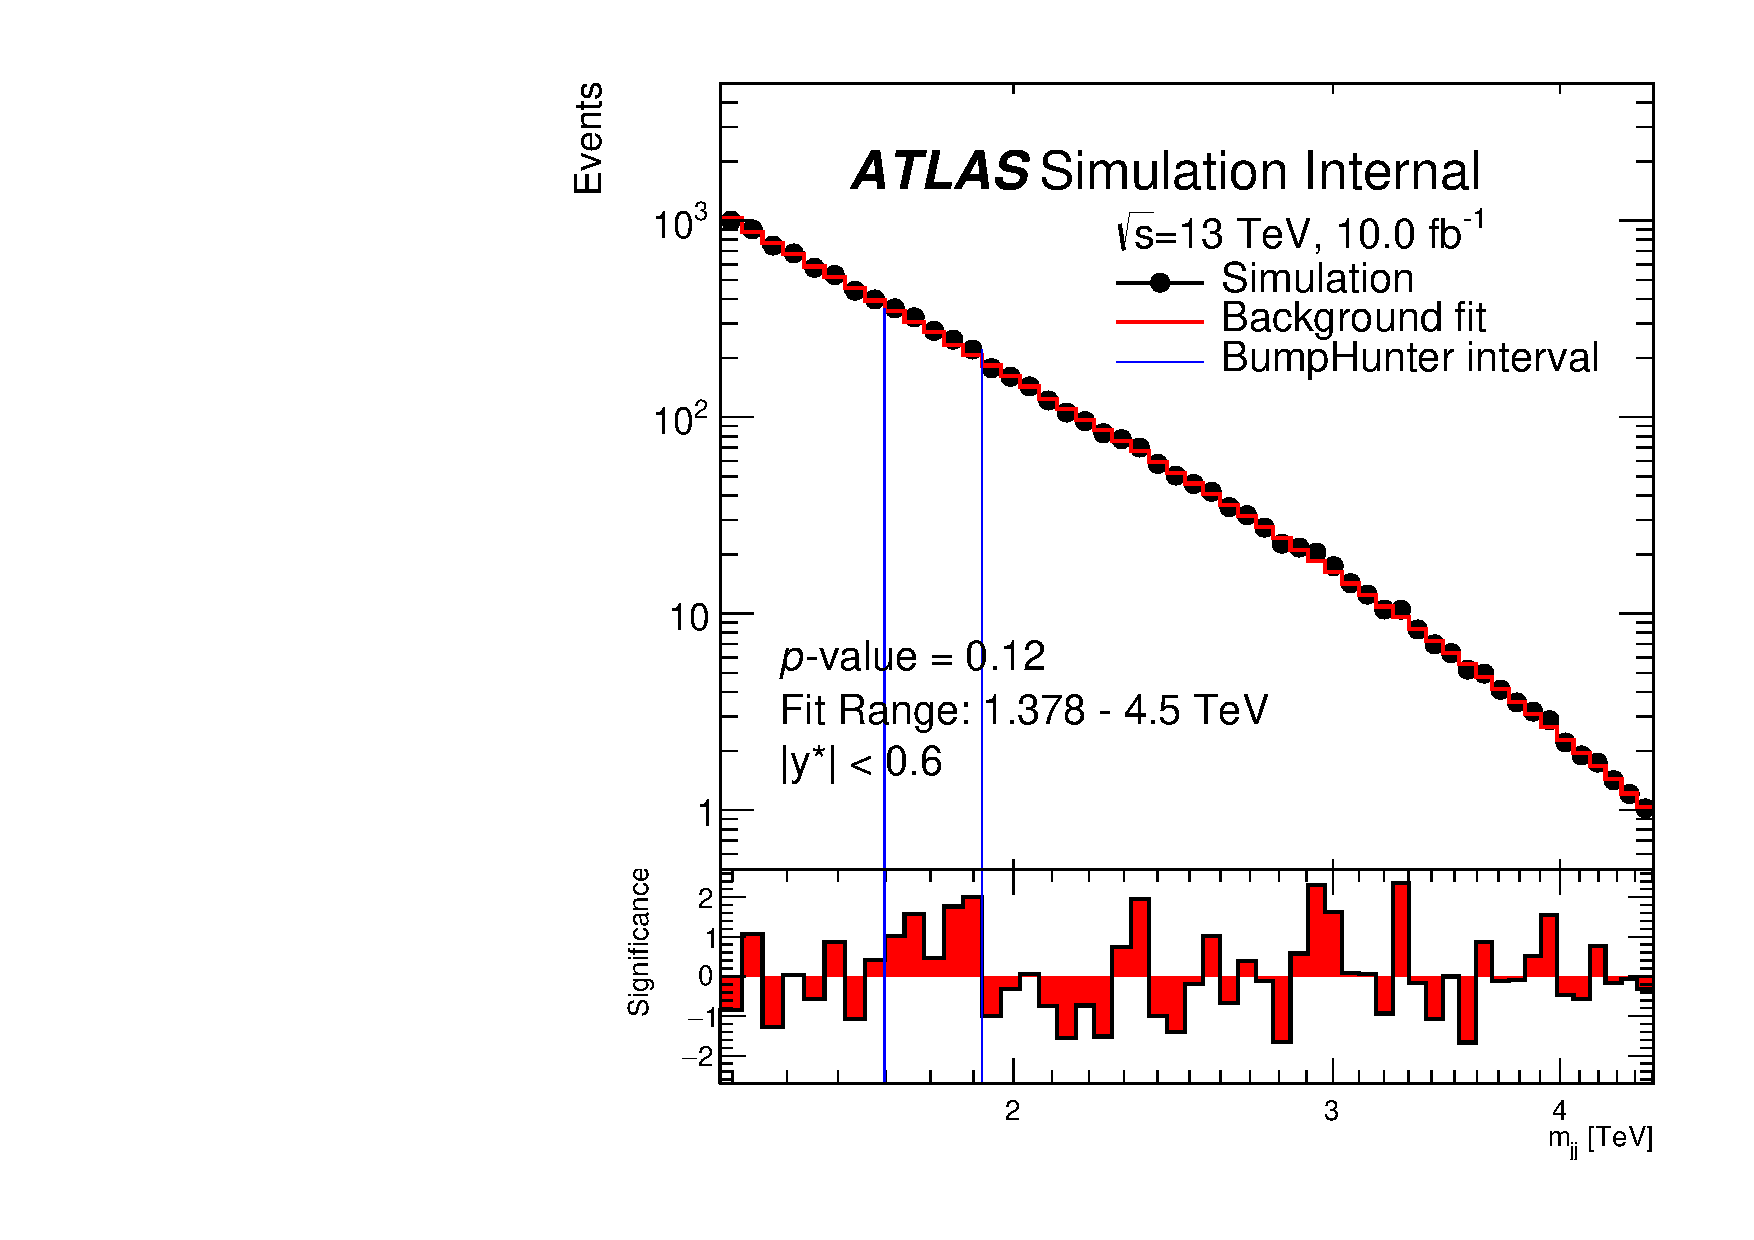
\includegraphics[width=0.47\linewidth, angle=0]{figs/Dibjet/ICHEP/FitRange/mbb_fix_8585_Short_4para_1378_figure1_10fb.pdf}}
   \subcaptionbox{$\geq$1 $b$-tag}{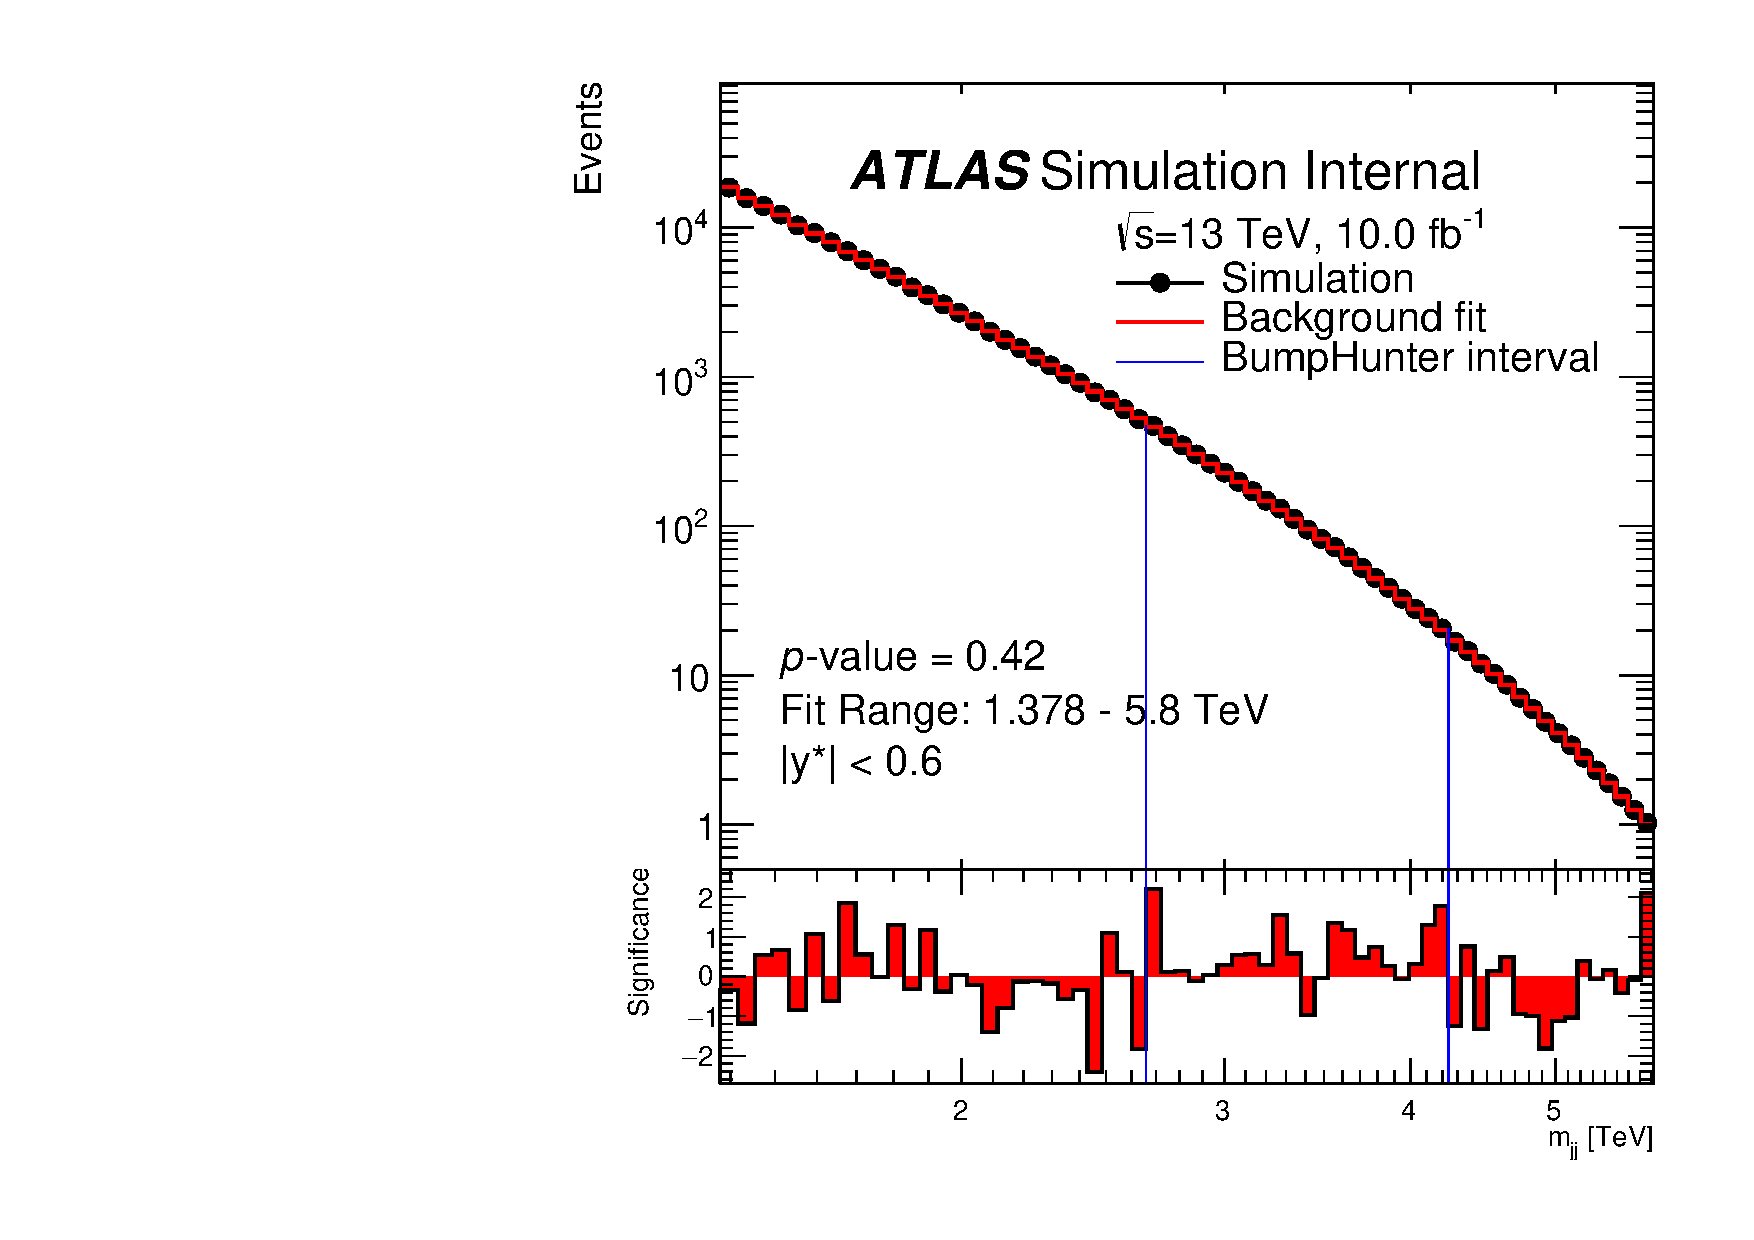
\includegraphics[width=0.47\linewidth, angle=0]{figs/Dibjet/ICHEP/FitRange/mbj_inc_fix_8585_Short_4para_1378_figure1_10fb.pdf}}
  \end{center}
  \caption{ The dijet mass distribution taken from multi-jet simulation for the (a) 2 $b$-tag and (b) $\geq$1 $b$-tag,
    category, fitted to using the 4 parameter fit function, with lower mass bound of the fit range $m_{jj}$ = 1378 GeV.
    The \bh{} algorithm is run to identify the most discrepant excess, as indicated by the blue lines.
    Pseudo-experiments are used to assign the excess a \mbox{$p$-value}, which is shown on the plot. 
    The \summer{} data-set event selection has been applied.}
  \label{fig:Short_4para_1378_figure1}
\end{figure}

%\begin{figure}[!ht]
%  \begin{center}
%    \captionsetup[subfigure]{aboveskip=0pt,justification=centering}
%   \subcaptionbox{2 $b$-tag}{
%      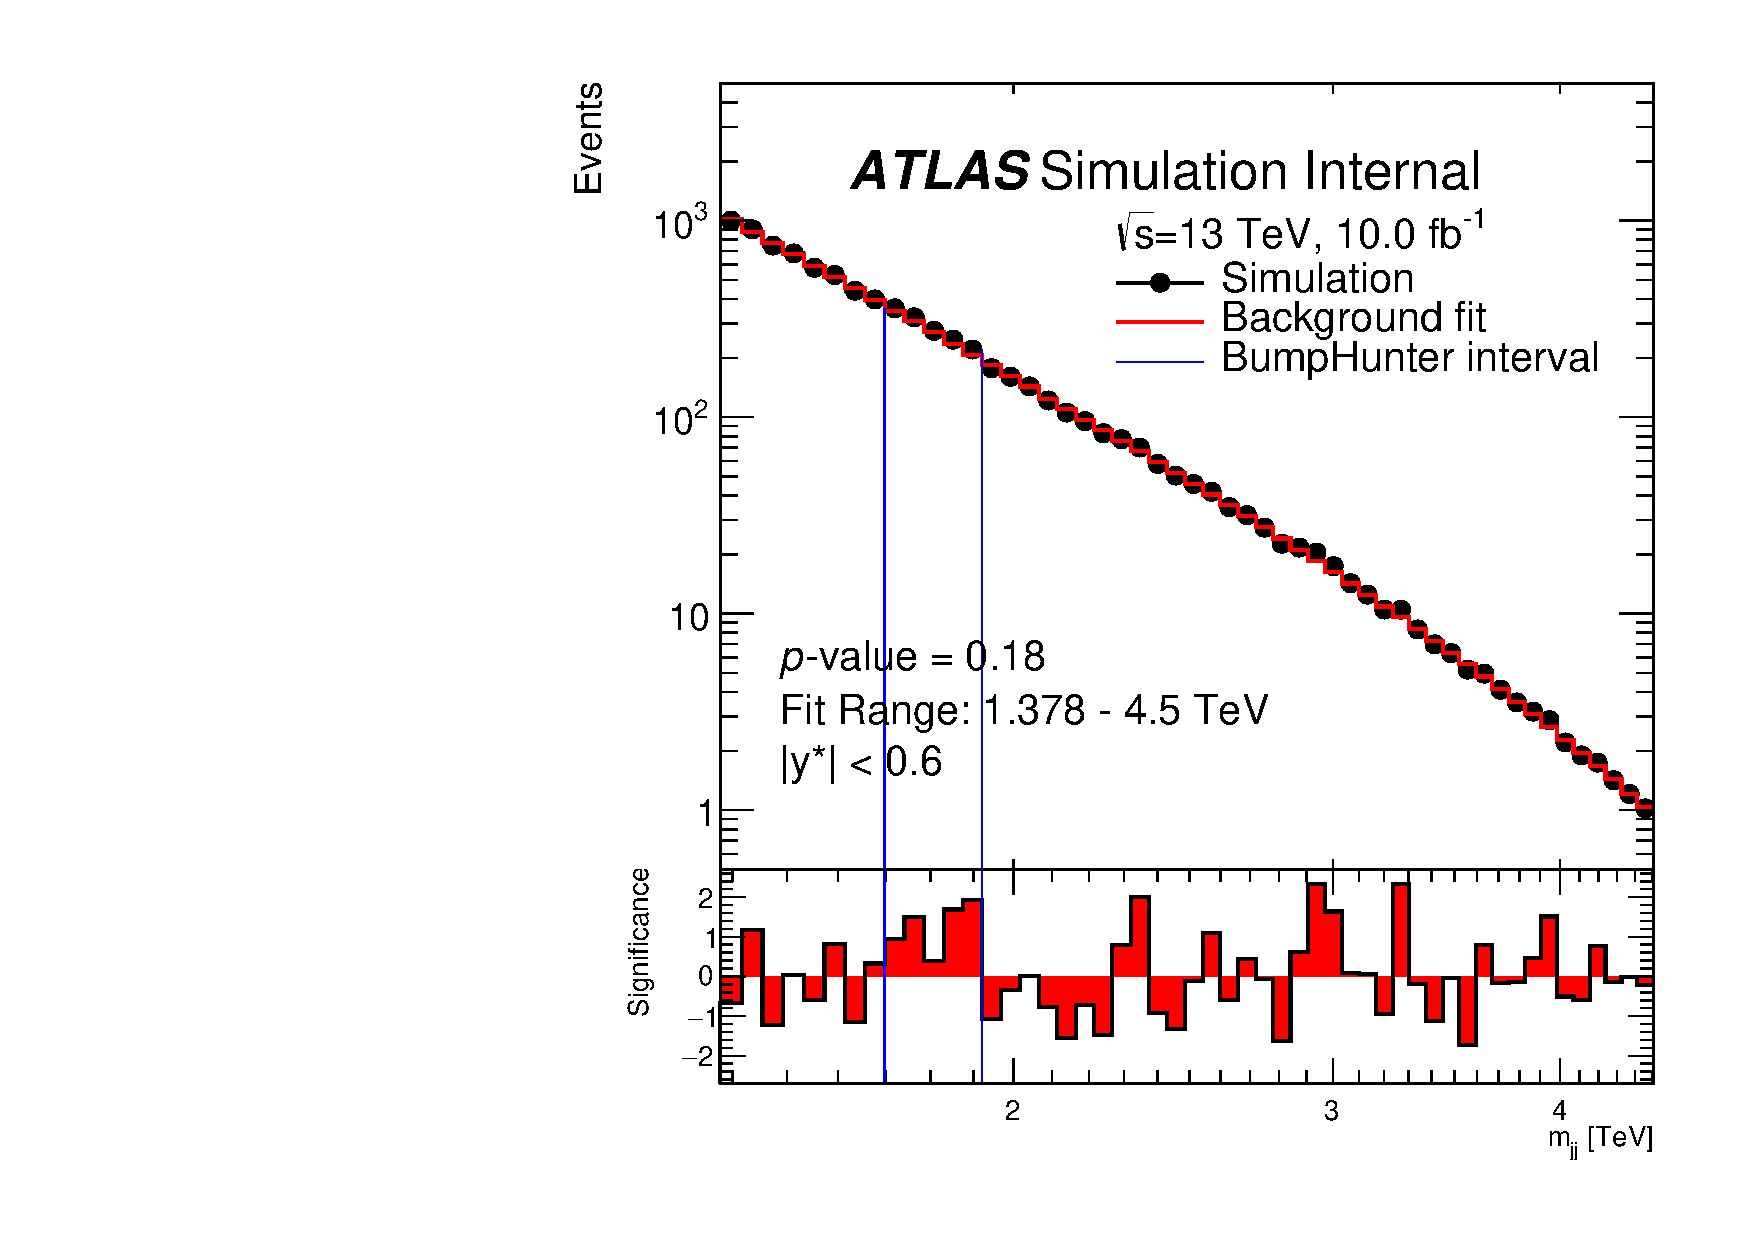
\includegraphics[width=0.47\linewidth, angle=0]{figs/Dibjet/ICHEP/FitRange/mbb_fix_8585_Short_5para_1378_figure1_10fb.pdf}
%    }
%   \subcaptionbox{$\geq$1 $b$-tag}{
%      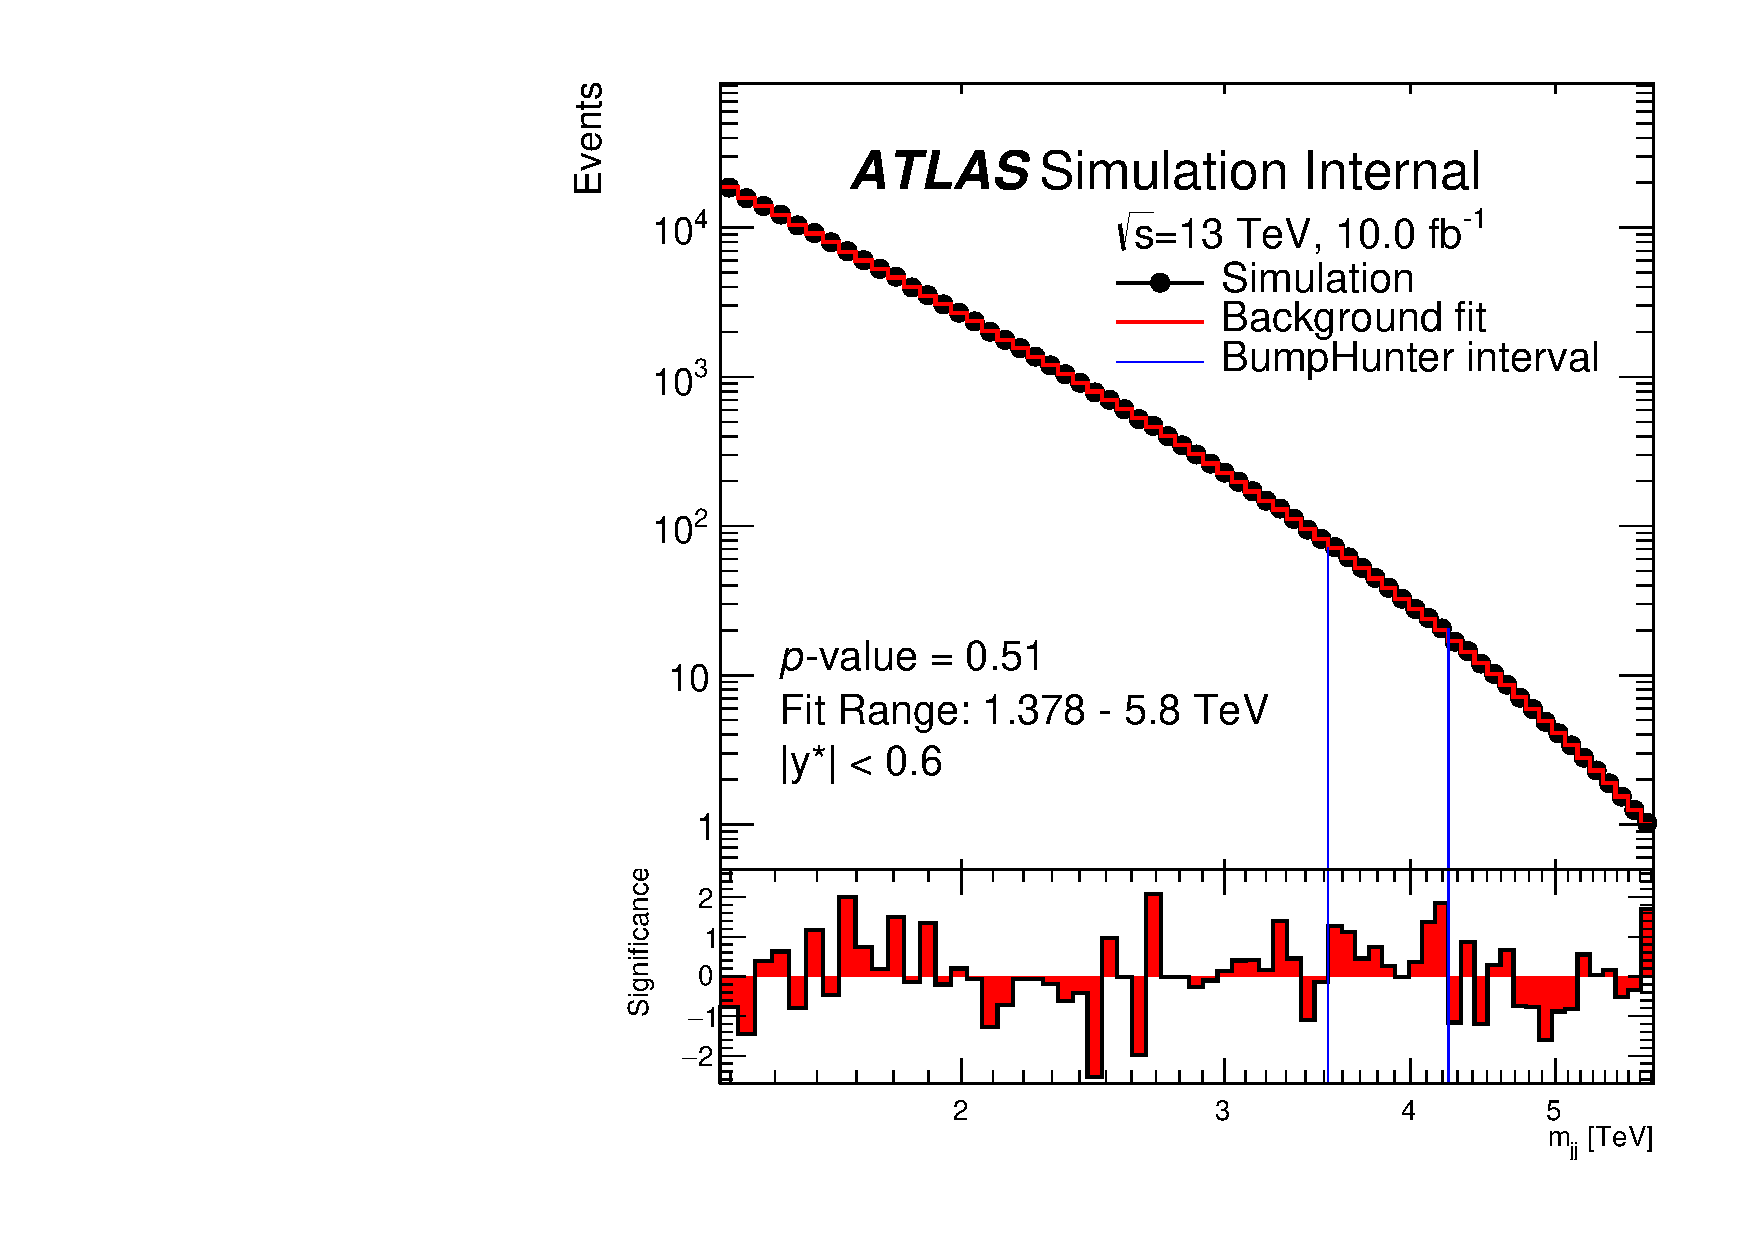
\includegraphics[width=0.47\linewidth, angle=0]{figs/Dibjet/ICHEP/FitRange/mbj_inc_fix_8585_Short_5para_1378_figure1_10fb.pdf}
%    }
%  \end{center}
%  \caption{ for the (a) 2 $b$-tag and (b) $\geq$1 $b$-tag category.}
%  \label{fig:}
%\end{figure}

\FloatBarrier
\subsection{Fit Tests: Spurious Signal}
\label{sec:bkg-summer_spusig}

In an inadequate background estimation strategy fit biases can occur,
where a fit bias is defined as differences between the the true background
dijet mass spectrum and the background estimation.
If fit biases could appear as false signal or could hide a true signal, the former is referred to as spurious signal.
To demonstrate that the background estimation strategy provides a valid representation of the true background spectrum
and that fit biases are not occurring, fits are performed to a background-only representative data-set.
Similar tests have been performed in previous iterations of both the inclusive and $b$-tagged dijet searches~\cite{dijet-mori16_paper,dibjet-mori16_paper}.

To perform these tests, the scaled distribution from the {\sc Pythia}8 Monte-Carlo multi-jet simulation
described in Section~\ref{sec:bkg-summer_fitCR}
is used as the representative background-only data-set.
%In Section~\ref{sec:FitStudies:FitRegion}
%the dijet mass spectrum used took the square root of the
%number of effective entries as the errors.
As shown in Figure~\ref{fig:effEnt},
the number of effective entries is larger than the number of scaled entries,
meaning that the distribution contains smaller statistical fluctuations than are present in the final data-set.
To create a more representative simulated data-set to test the fit functions,
Poisson fluctuations are applied to the scaled distribution to create a `data-like' distribution.
Figure~\ref{fig:effEntDataLike} shows the scaled and effective entries distributions for both
$b$-tag categories overlaid with a data-like distribution in blue.

\begin{figure}[!ht]
  \begin{center}
   \captionsetup[subfigure]{aboveskip=0pt,justification=centering}
    \subcaptionbox{2 $b$-tag}{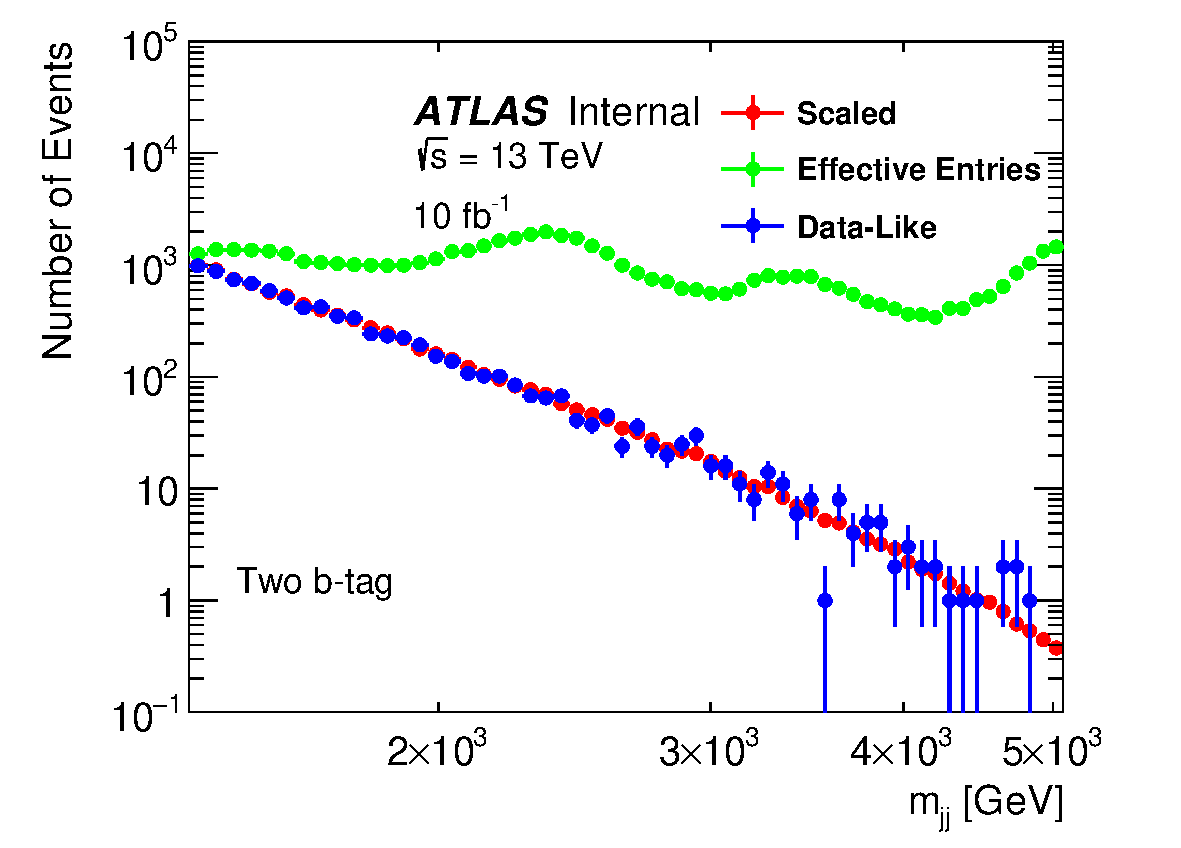
\includegraphics[width=0.47\linewidth, angle=0]{figs/Dibjet/ICHEP/SpuriousSignal/mbb_fix_8585_dataLike_effEntries_Logx_10fb.pdf}\label{fig:effEntDataLike_bb}}
    \subcaptionbox{$\geq$1 $b$-tag}{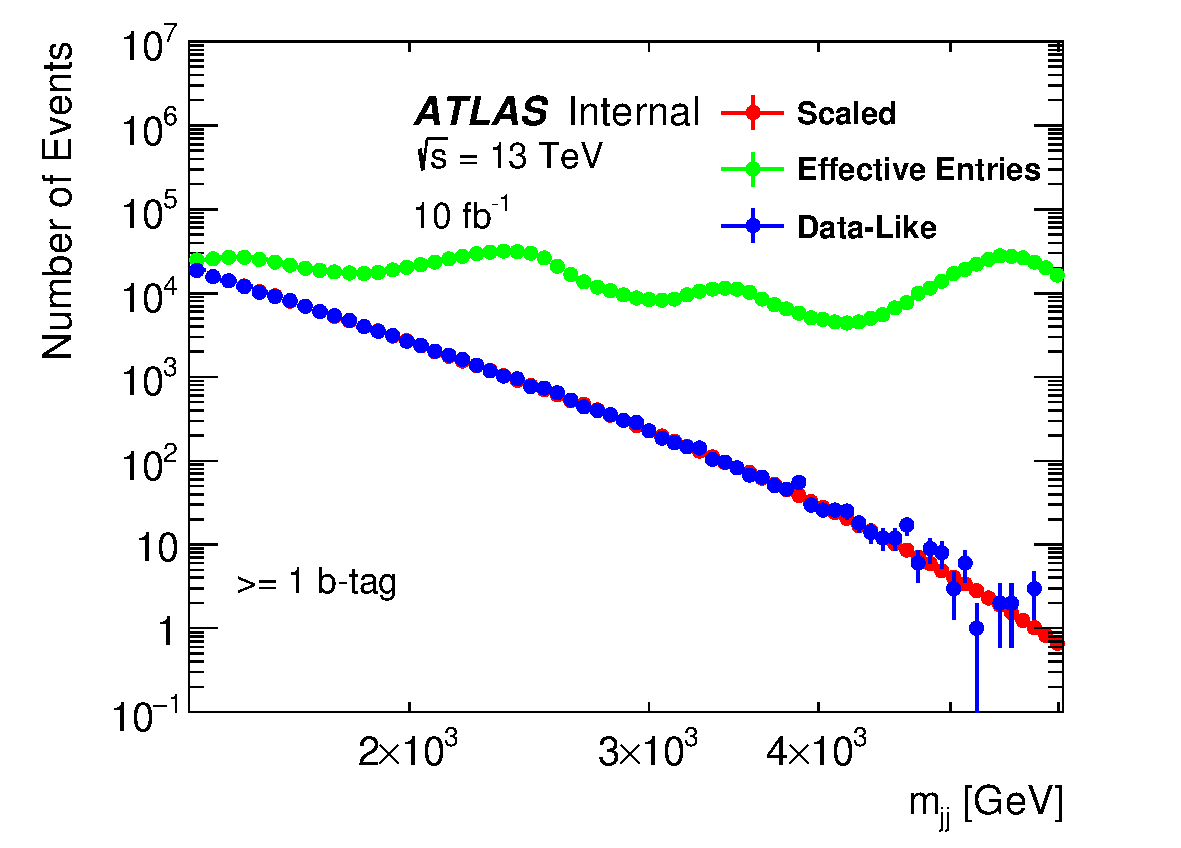
\includegraphics[width=0.47\linewidth, angle=0]{figs/Dibjet/ICHEP/SpuriousSignal/mbj_inc_fix_8585_dataLike_effEntries_Logx_10fb.pdf}\label{fig:effEntDataLike_bj}}
  \end{center}
  \caption{The scaled dijet mass distribution (red) compared to the
    effective entries of the dijet mass distribution (green) for the 2 $b$-tag category,
    for the (a) 2 $b$-tag and (b) $\geq$1 $b$-tag case.
    Overlaid is a data-like distribution (blue) created by applying Poisson fluctuations to the scaled distribution.
    The \summer{} data-set event selection has been applied.}
  \label{fig:effEntDataLike}
\end{figure}

The search phase is then applied to the data-like distributions
in both $b$-tag categories 
to test the fit function in a background-only data-set.
Figure~\ref{fig:DataLikeSearchPhase} shows an example data-like distribution for both $b$-tag categories fitted
to with the 3 parameter fit function,
with the most discrepant excess as identified by the \bh{} algorithm shown.
The \mbox{$p$-value} of the most discrepant excess is calculated by comparing the \bh{} test statistic in the data-like distribution, $t_{obs}$,
to 10,000 pseudo-experiments; the procedure is illustrated in Figure~\ref{fig:DataLikeStatPlots_bh}.
Using a similar process, the \mbox{$p$-value} of the most discrepant deficit is calculated using the \dhunt{} test statistic
and an overall quality of fit \mbox{$p$-value} is calculated by the $\chi^{2}$ test statistic.
For this specific set of Poisson fluctuations in the 2 $b$-tag category
the \bh{}, \dhunt{} and  $\chi^{2}$ \mbox{$p$-value} are found to be
0.57, 0.80 and 0.39 respectively.
Similarly, in the $\geq1$ $b$-tag category the
\bh{}, \dhunt{} and  $\chi^{2}$ \mbox{$p$-value}s are
0.93, 0.77 and 0.86 respectively.
Therefore, the fit is performing well for both $b$-tagging categories for this data-like distribution.

\begin{figure}[!ht]
  \begin{center}
   \captionsetup[subfigure]{aboveskip=0pt,justification=centering}
    \subcaptionbox{2 $b$-tag}{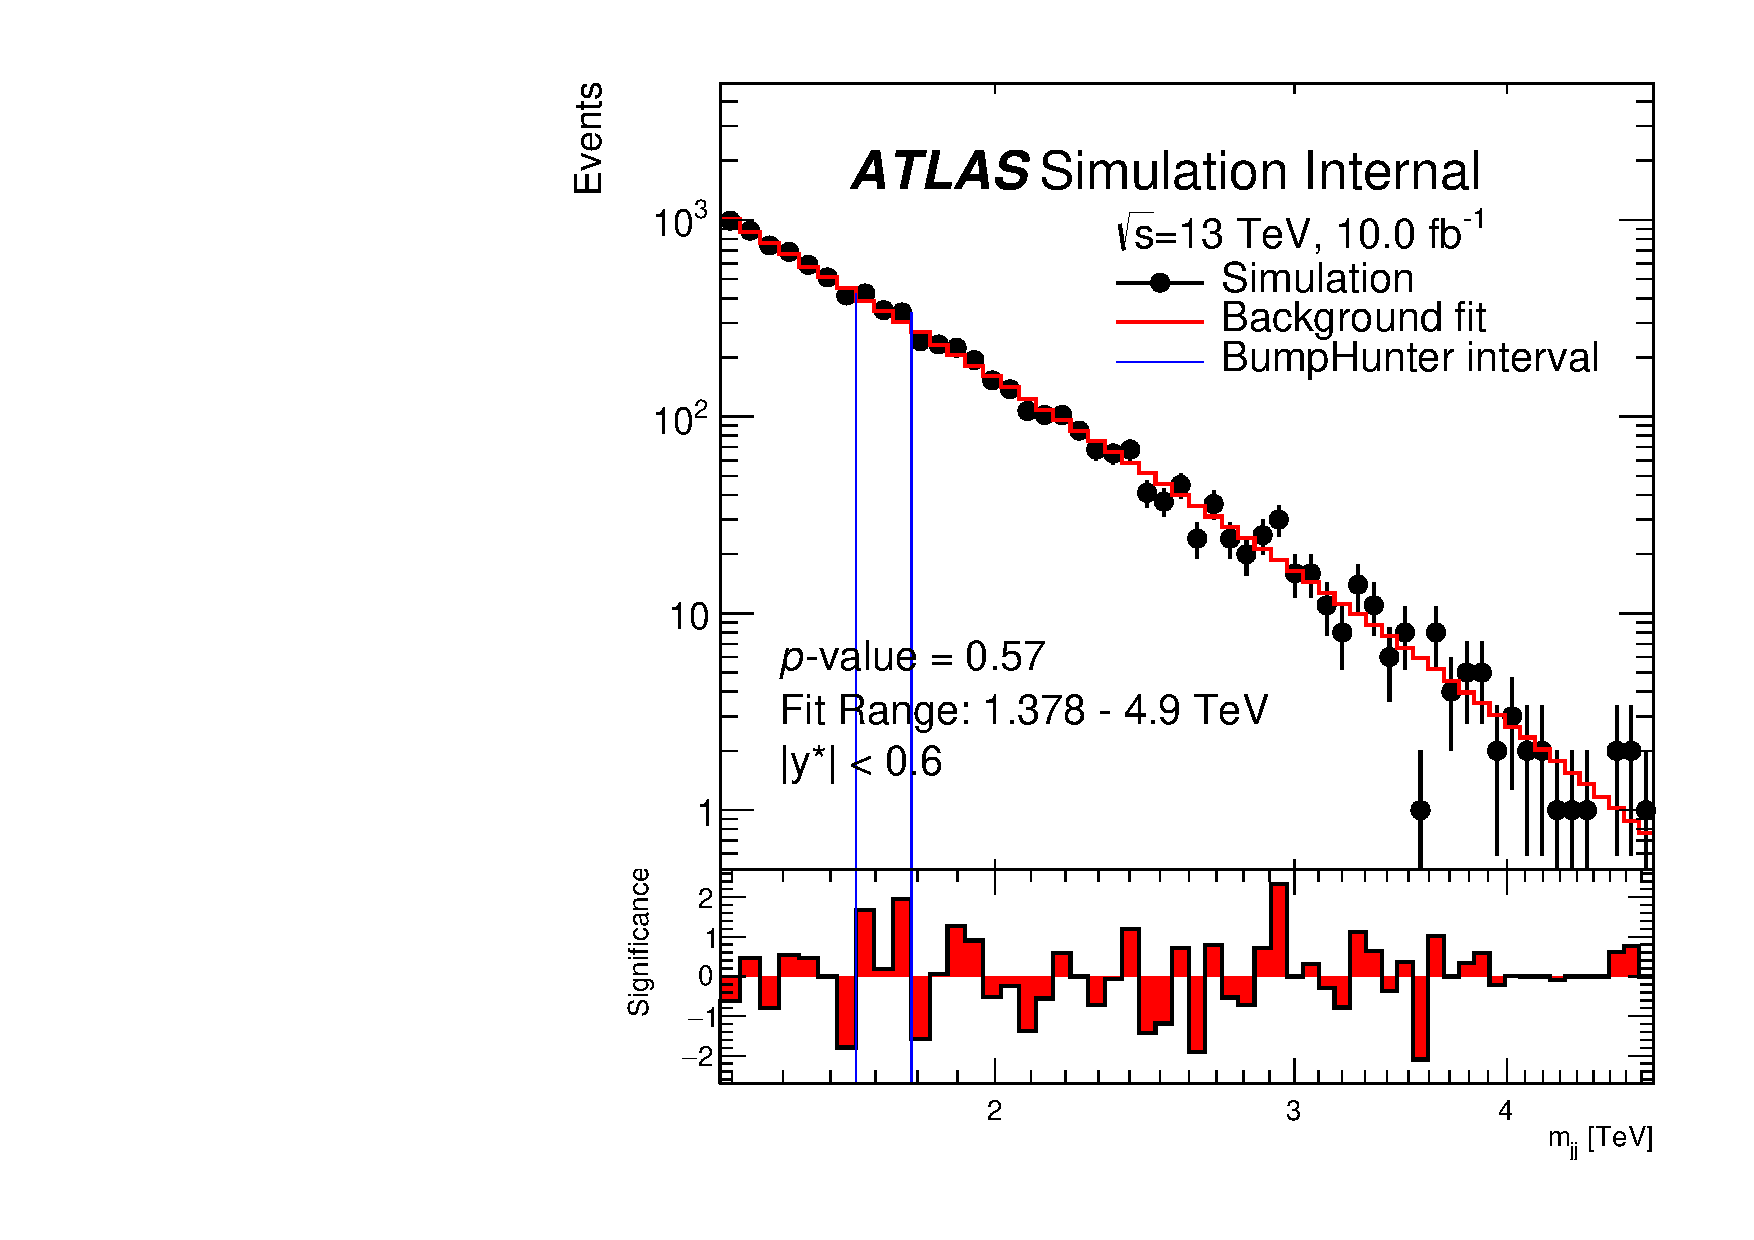
\includegraphics[width=0.47\linewidth, angle=0]{figs/Dibjet/ICHEP/SpuriousSignal/mbb_fix_8585_figure1_10fb_v10.pdf}}
    \subcaptionbox{$\geq$1 $b$-tag}{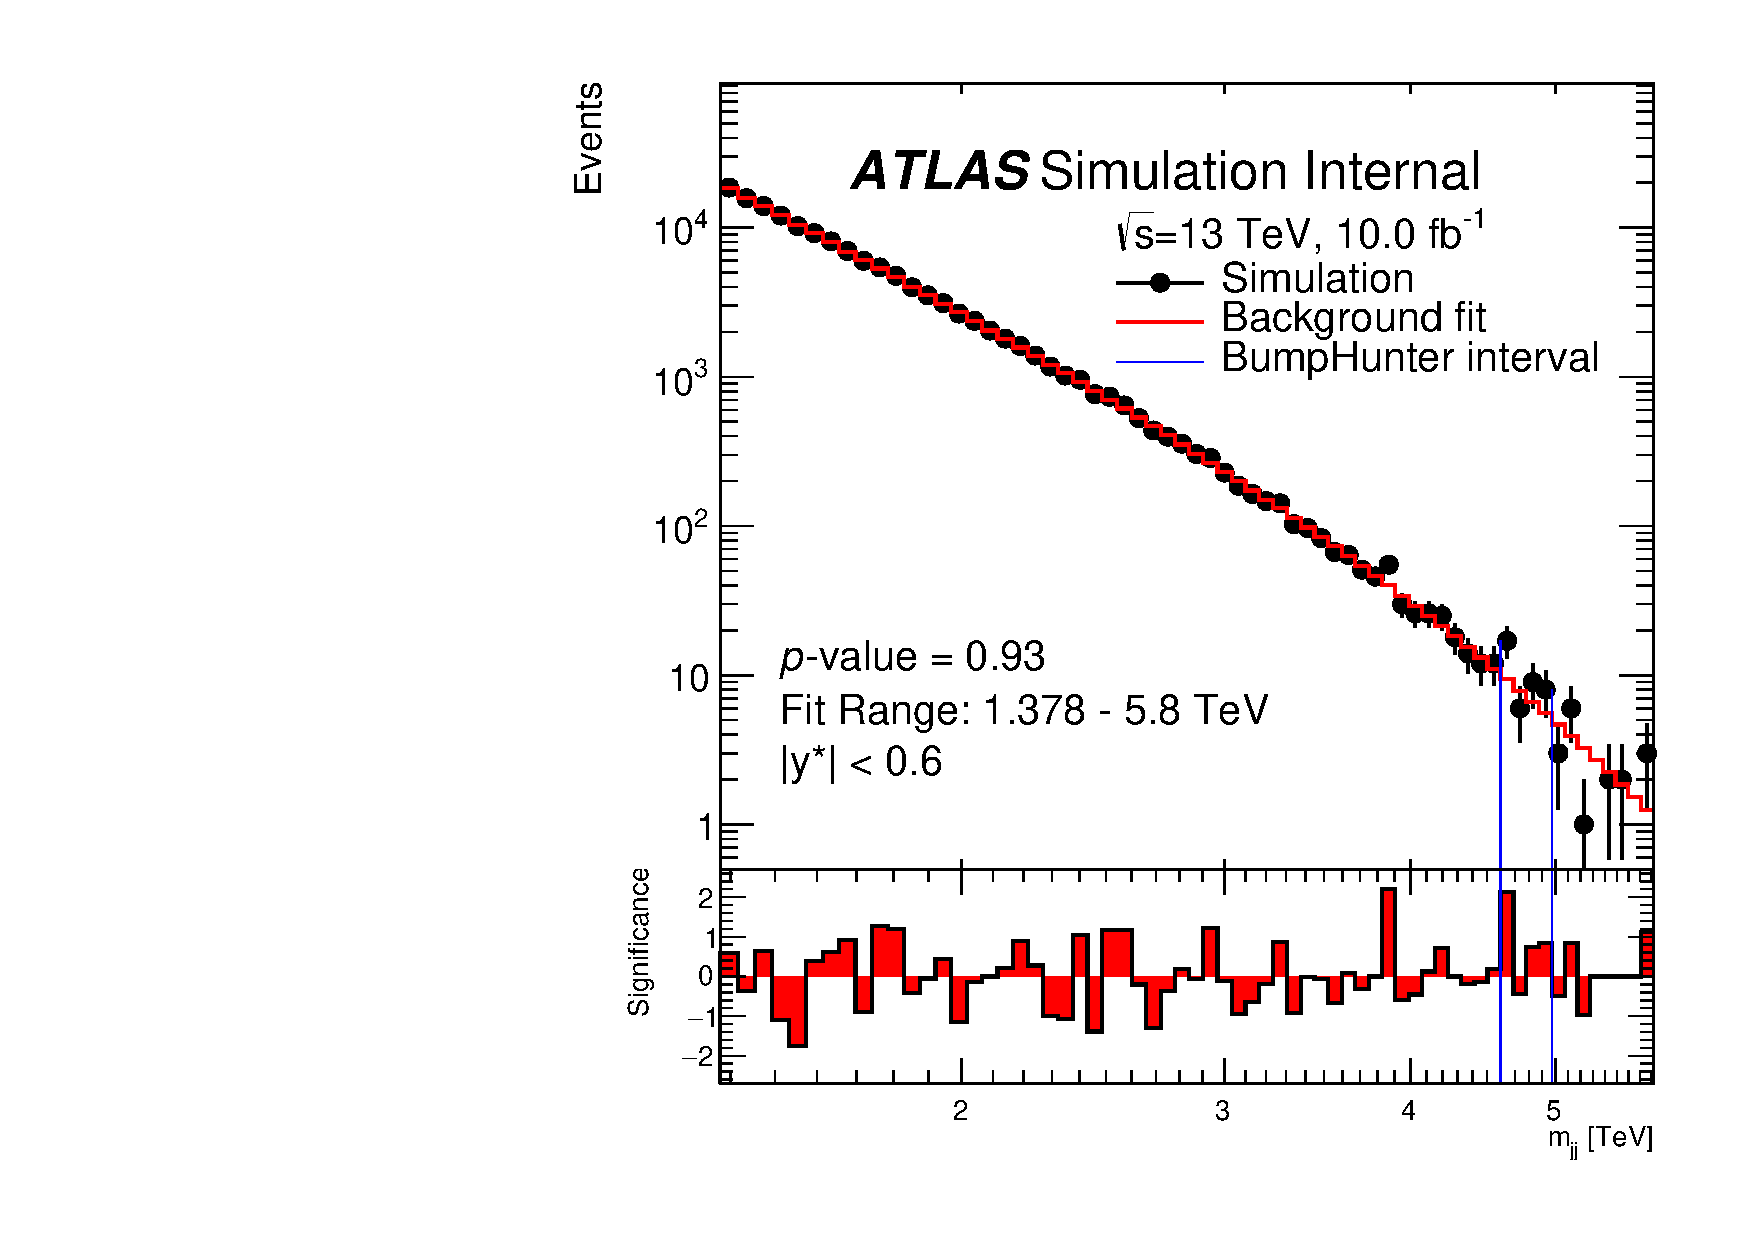
\includegraphics[width=0.47\linewidth, angle=0]{figs/Dibjet/ICHEP/SpuriousSignal/mbj_inc_fix_8585_figure1_10fb_v10.pdf}}
  \end{center}
  \caption{A data-like distribution taken from multi-jet simulation for the (a) 2 $b$-tag and (b) $\geq$1 $b$-tag,
    category, fitted to using the 3 parameter fit function.
    The \bh{} algorithm is run to identify the most discrepant excess, as indicated by the blue lines.
    Pseudo-experiments are used to assign the excess a \mbox{$p$-value}, which is shown on the plot.
    The \summer{} data-set event selection has been applied.}
  \label{fig:DataLikeSearchPhase}
\end{figure}

\begin{figure}[!ht]
  \begin{center}
    \captionsetup[subfigure]{aboveskip=0pt,justification=centering}
    \subcaptionbox{2 $b$-tag}{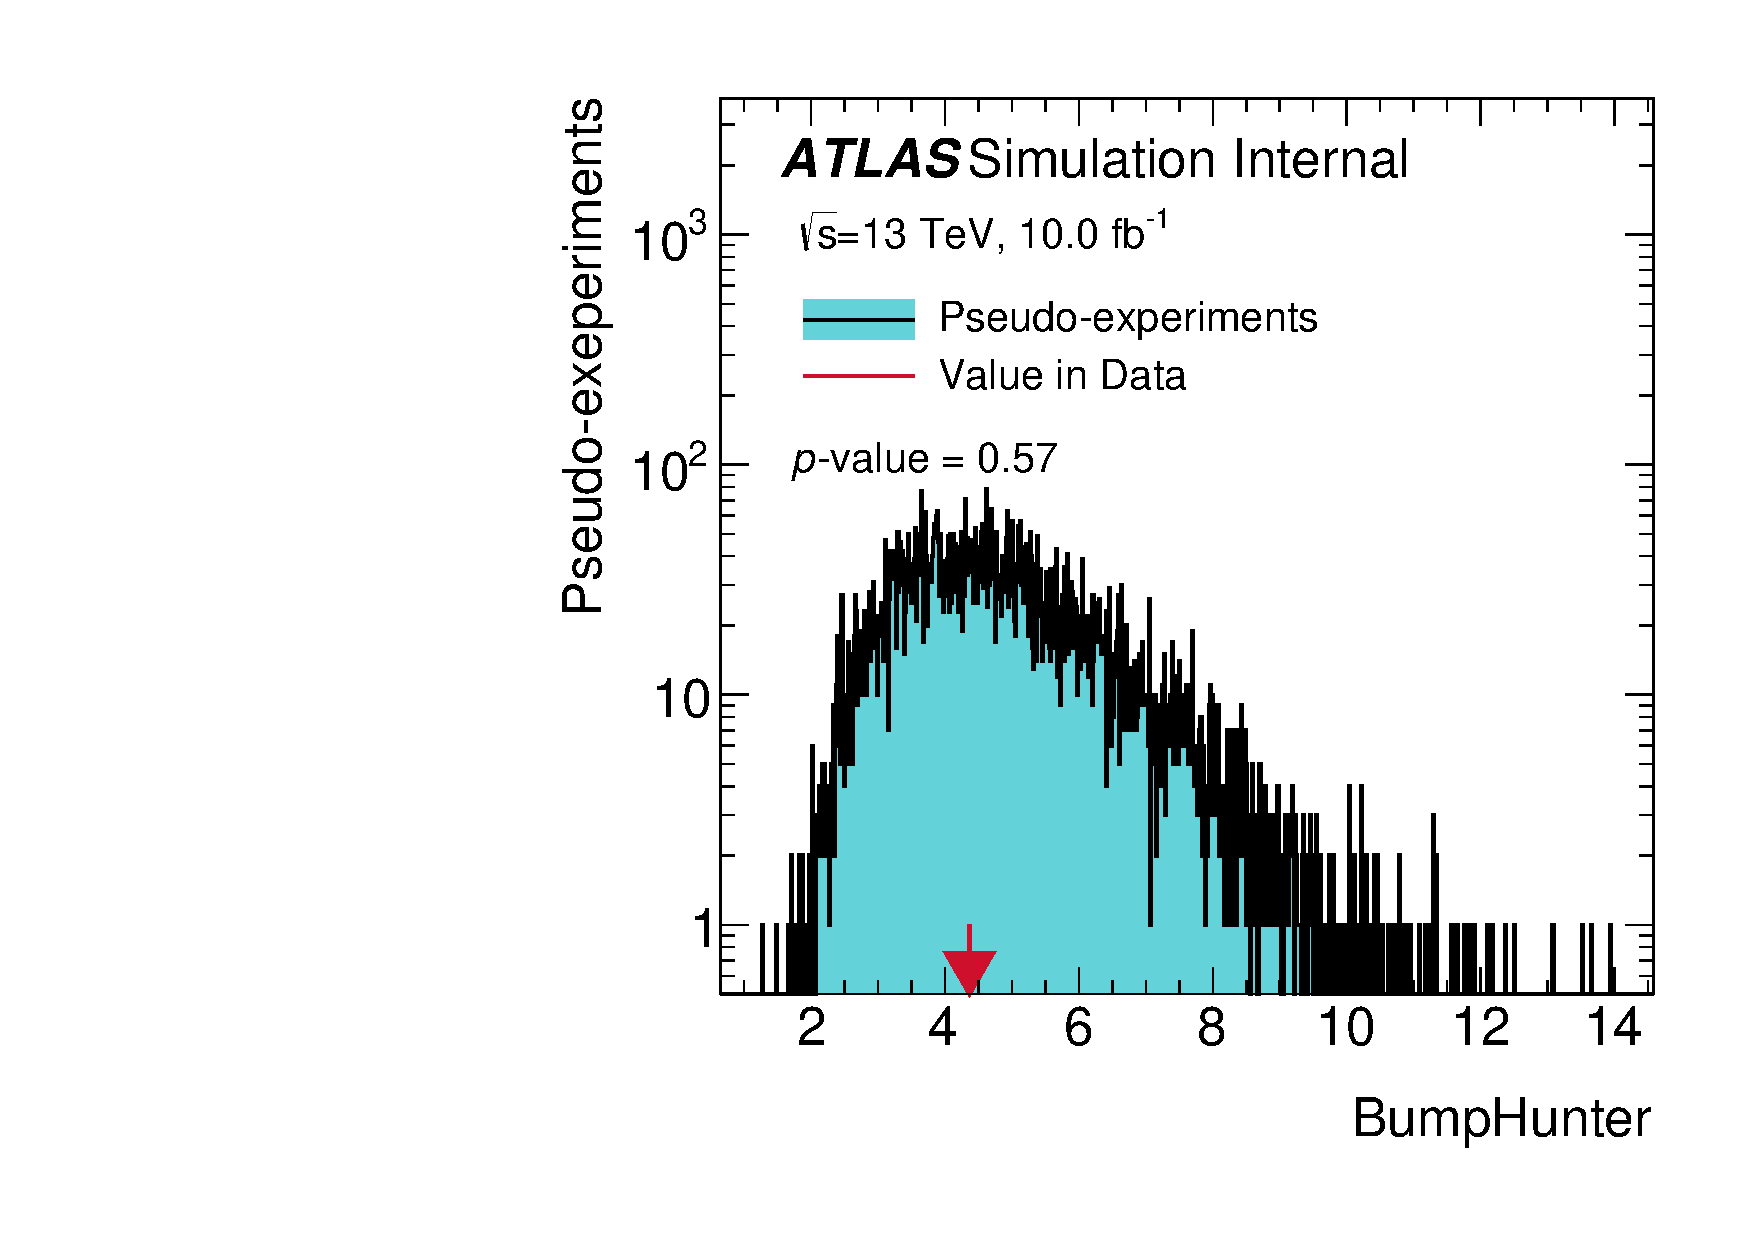
\includegraphics[width=0.47\linewidth, angle=0]{figs/Dibjet/ICHEP/SpuriousSignal/mbb_fix_8585_bumpHunterStatPlot_10fb_v10.pdf}\label{fig:DataLikeBumpHunterStatPlot_bb}}
    \subcaptionbox{$\geq$1 $b$-tag}{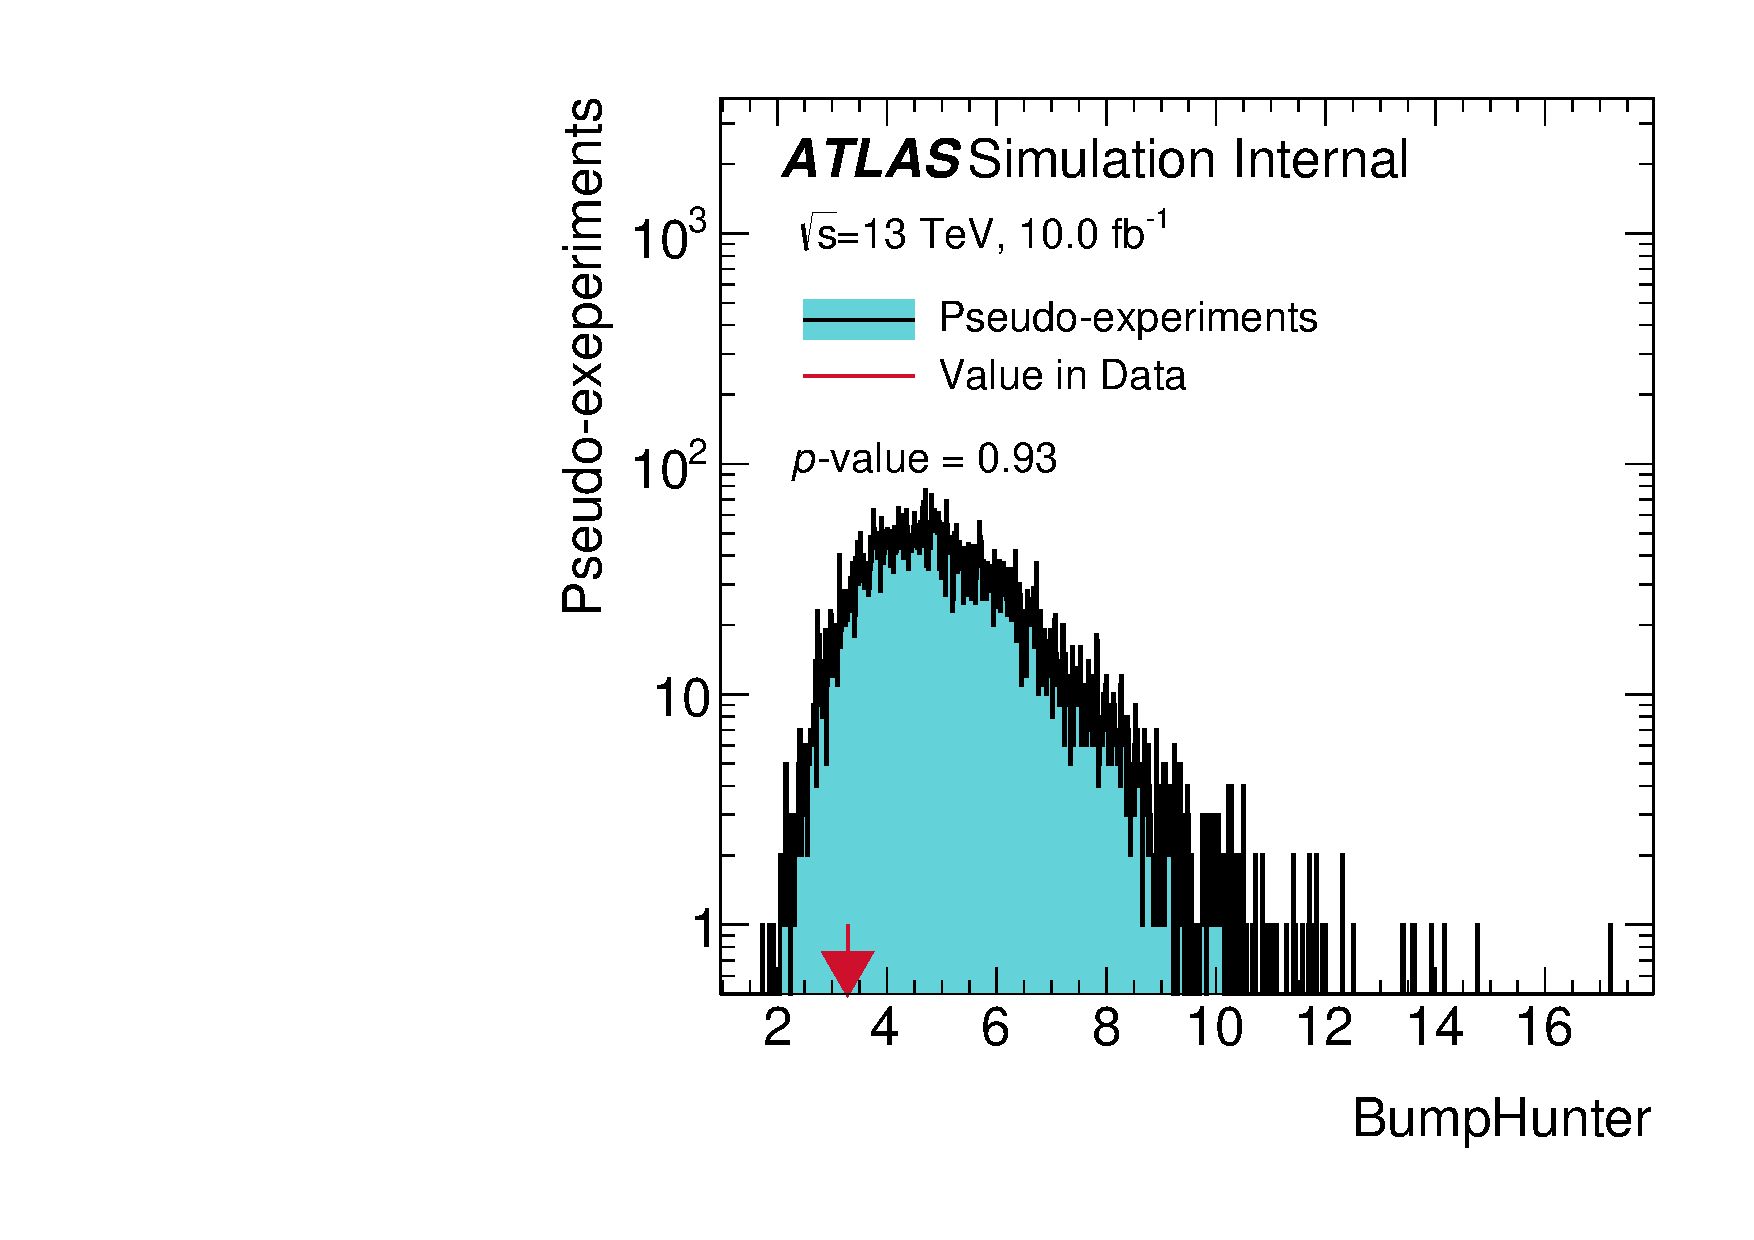
\includegraphics[width=0.47\linewidth, angle=0]{figs/Dibjet/ICHEP/SpuriousSignal/mbj_inc_fix_8585_bumpHunterStatPlot_10fb_v10.pdf}\label{fig:DataLikeBumpHunterStatPlot_bj}}
  \end{center}
  \caption{The distribution of the \bh{} test statistic for 10,000 pseudo experiments compared
    to the value observed in a data-like distribution from the (a) 2 $b$-tag category and (b) $\geq$1 $b$-tag category.
    The fraction of pseudo-experiments with a \bh{} test statistic greater than the value in data is the estimation of the respective \mbox{$p$-value}.}
  \label{fig:DataLikeStatPlots_bh}
\end{figure}


%\begin{figure}[!ht]
%  \begin{center}
%   \captionsetup[subfigure]{aboveskip=0pt,justification=centering}
%  \subcaptionbox{\bh{}}{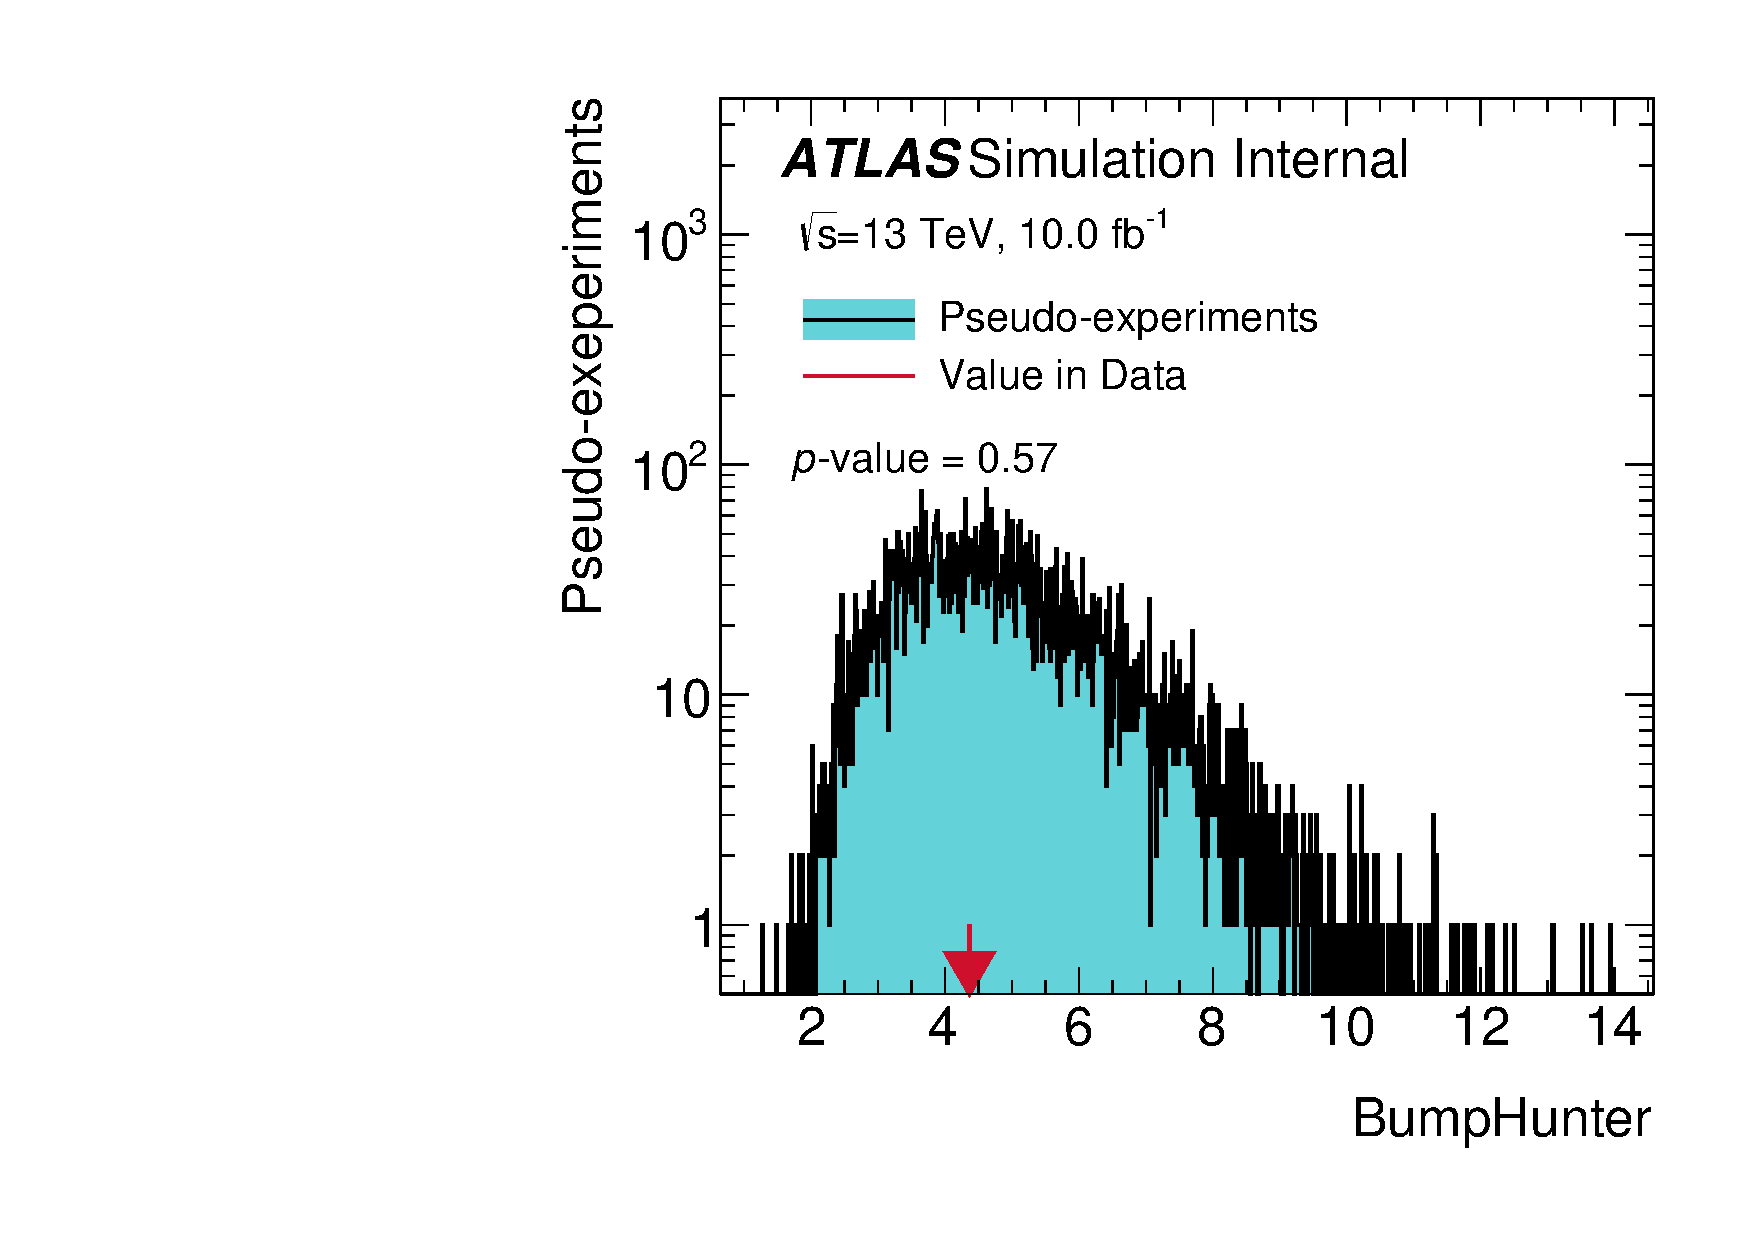
\includegraphics[width=0.47\linewidth, angle=0]{figs/Dibjet/ICHEP/SpuriousSignal/mbb_fix_8585_bumpHunterStatPlot_10fb_v10.pdf}\label{fig:DataLikeBumpHunterStatPlot_bb}}
%  \subcaptionbox{\dhunt{}}{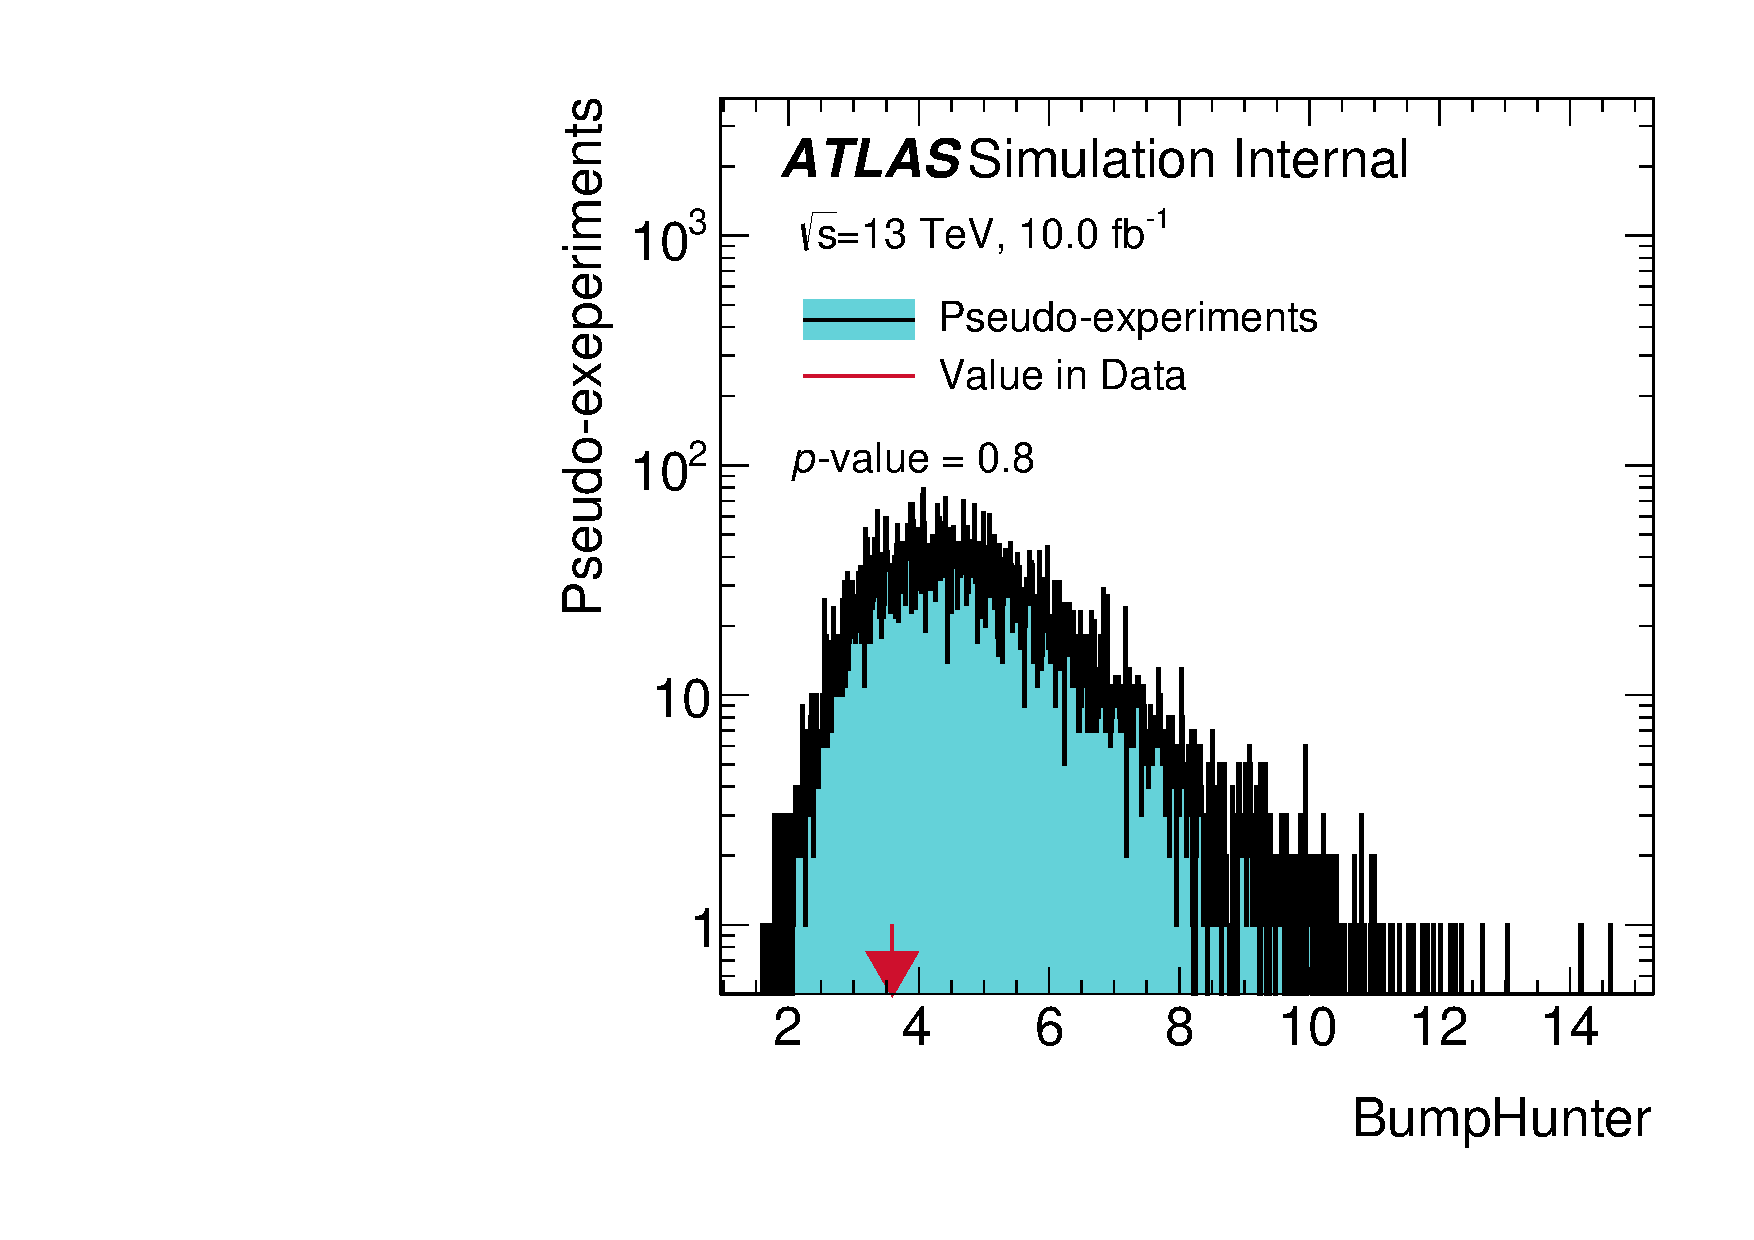
\includegraphics[width=0.47\linewidth, angle=0]{figs/Dibjet/ICHEP/SpuriousSignal/mbb_fix_8585_deficitOnlyHunterStatPlot_10fb_v10.pdf}\label{fig:DataLikeDeficitOnlyHunterStatPlot_bb}}  
%  \subcaptionbox{$\chi^{2}$}{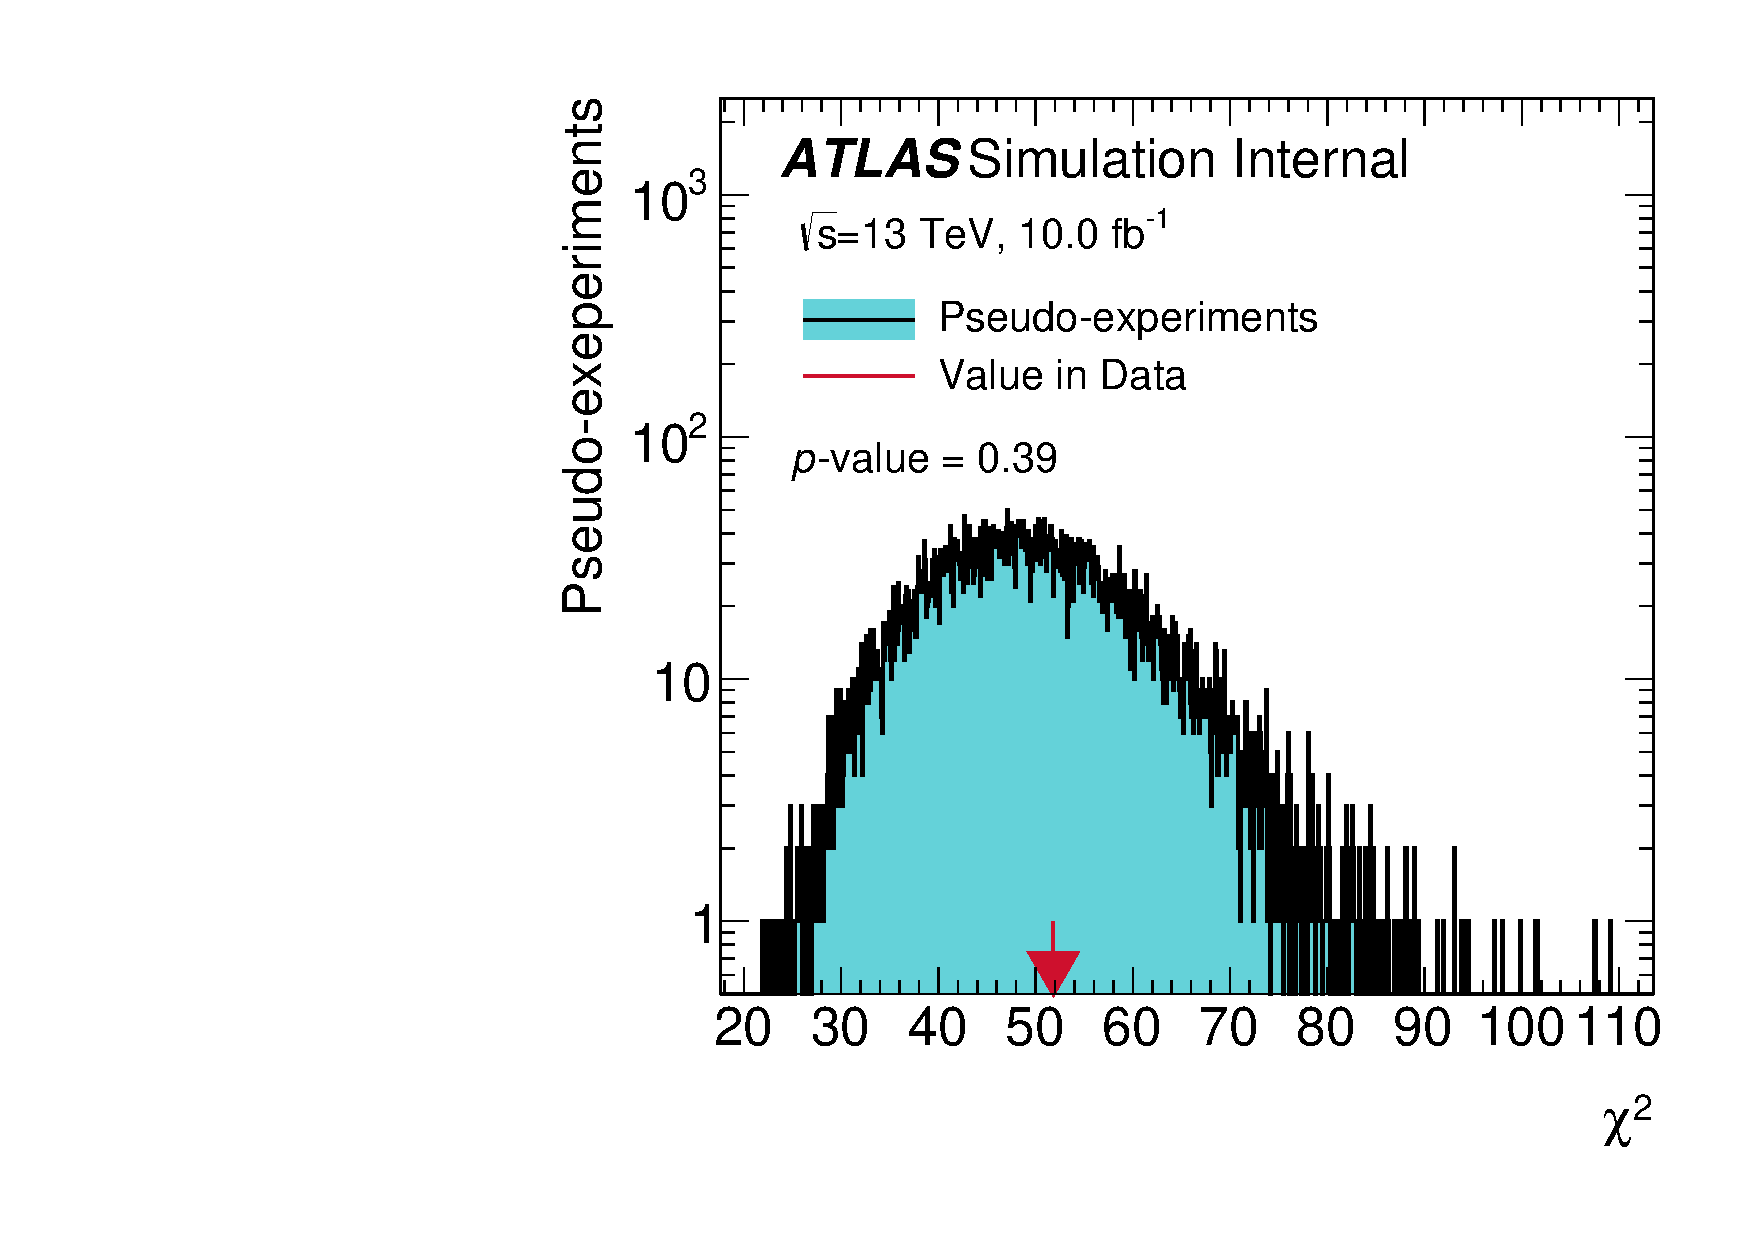
\includegraphics[width=0.47\linewidth, angle=0]{figs/Dibjet/ICHEP/SpuriousSignal/mbb_fix_8585_chi2StatPlot_10fb_v10.pdf}\label{fig:DataLikeChi2StatPlot_bb}}  
%  \end{center}
%  \caption{The distribution of the (a) \bh{} test statistic, (b) \dhunt{} test statistic and (c) $\chi^{2}$ test statistic for 10,000 pseudo experiments
%    compared to the value found in a data-like distribution for the 2 $b$-tag category. 
%    The fraction of pseudo-experiments with a \bh{}, \dhunt{} or $\chi^{2}$ test statistic greater than the value in data is the estimation of the respective \mbox{$p$-value}.}
%  \label{fig:DataLikeStatPlots_bb}
%  \begin{center}
%   \captionsetup[subfigure]{aboveskip=0pt,justification=centering}
%  \subcaptionbox{\bh{}}{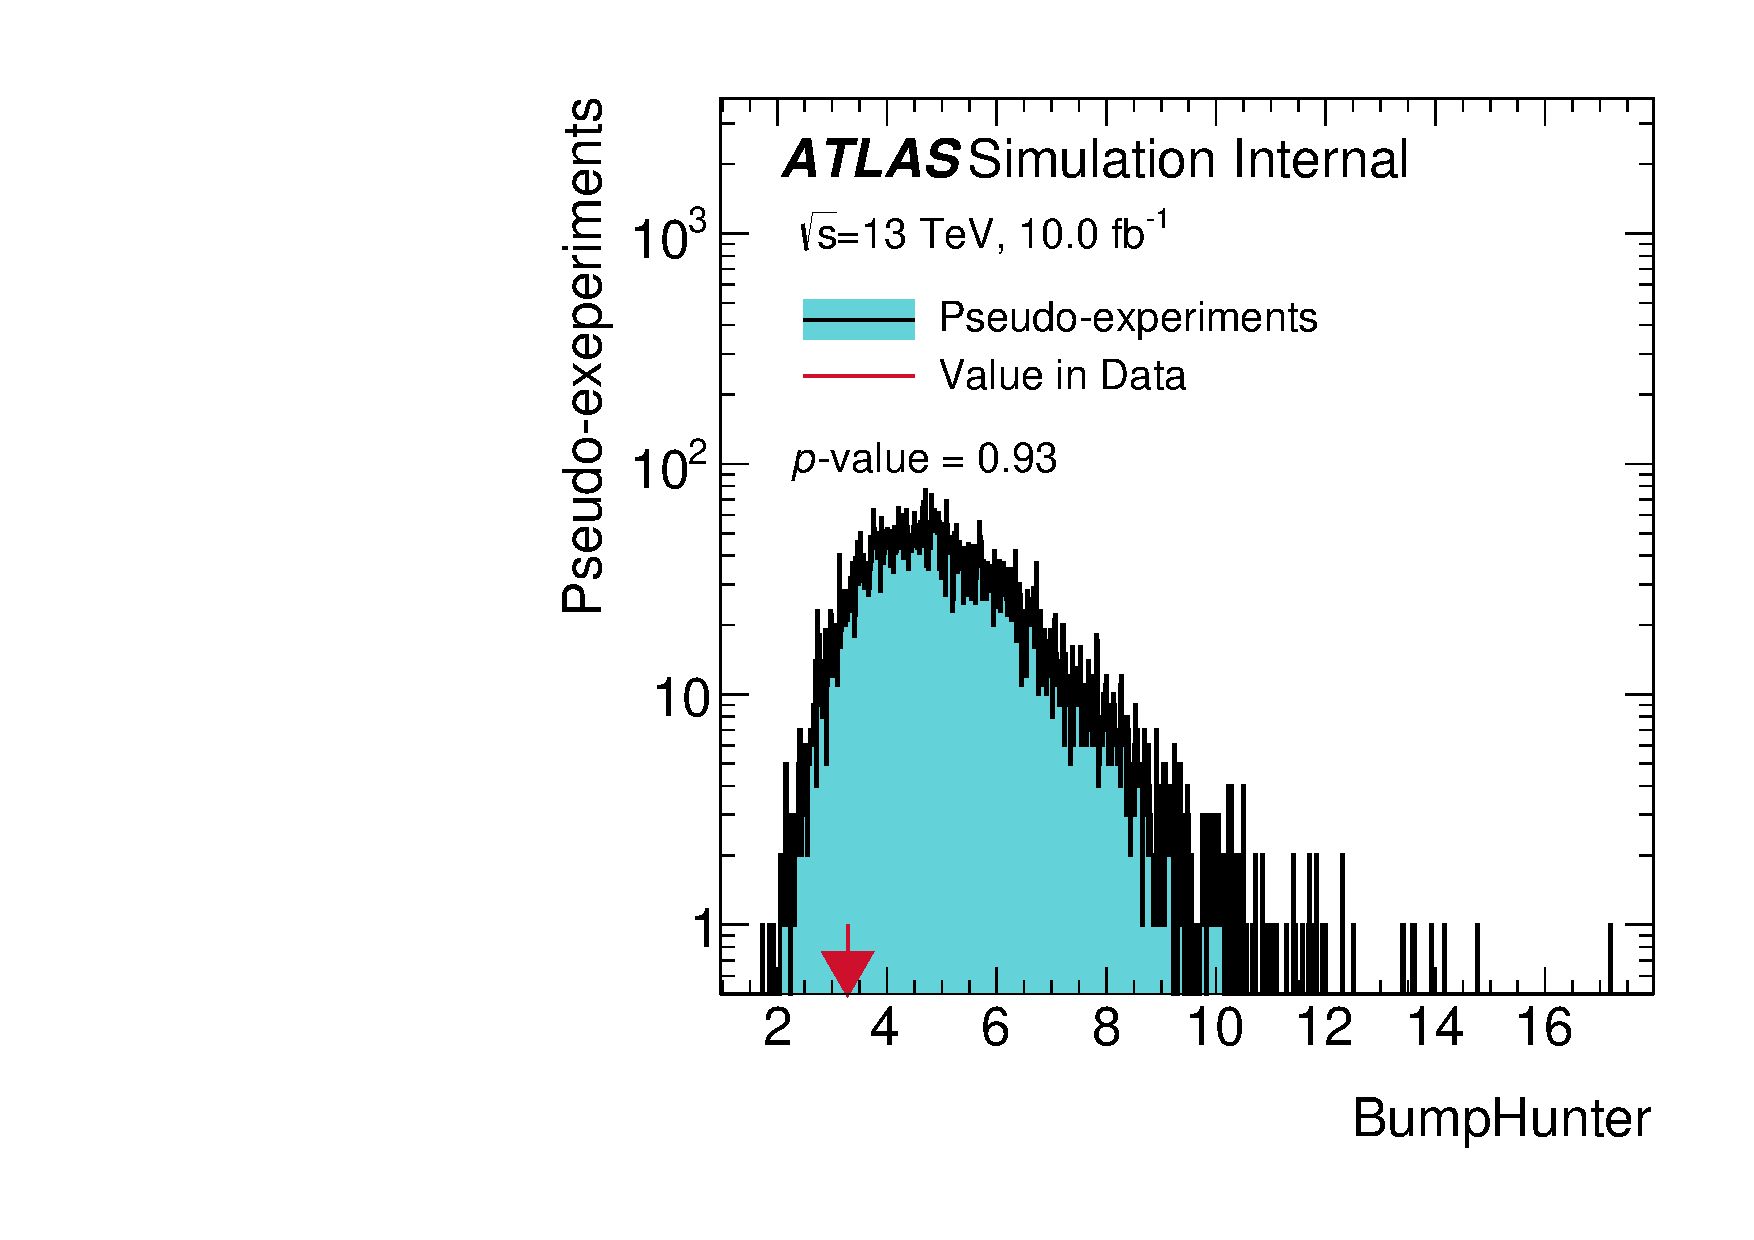
\includegraphics[width=0.47\linewidth, angle=0]{figs/Dibjet/ICHEP/SpuriousSignal/mbj_inc_fix_8585_bumpHunterStatPlot_10fb_v10.pdf}\label{fig:DataLikeBumpHunterStatPlot_bj}}
%  \subcaptionbox{\dhunt{}}{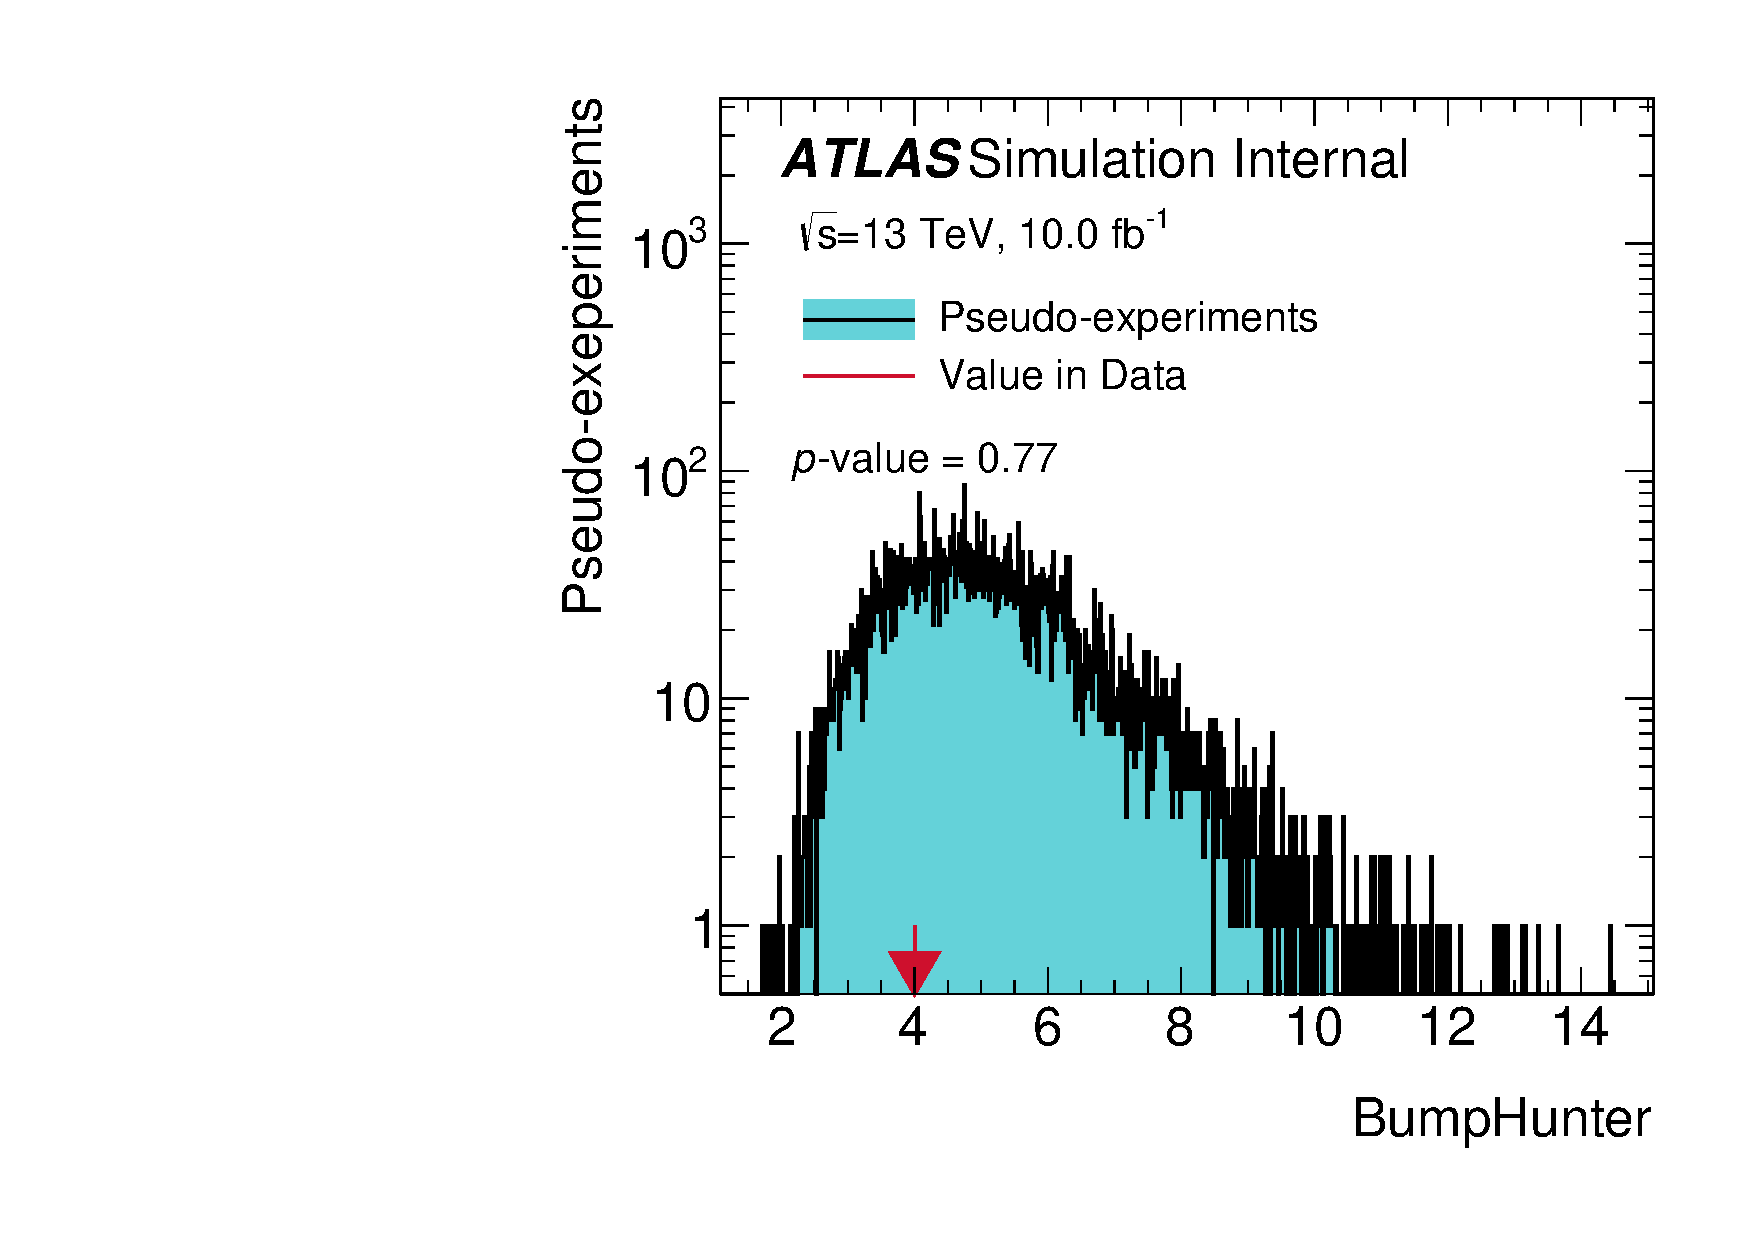
\includegraphics[width=0.47\linewidth, angle=0]{figs/Dibjet/ICHEP/SpuriousSignal/mbj_inc_fix_8585_deficitOnlyHunterStatPlot_10fb_v10.pdf}\label{fig:DataLikeDeficitOnlyHunterStatPlot_bj}}  
%  \subcaptionbox{$\chi^{2}$}{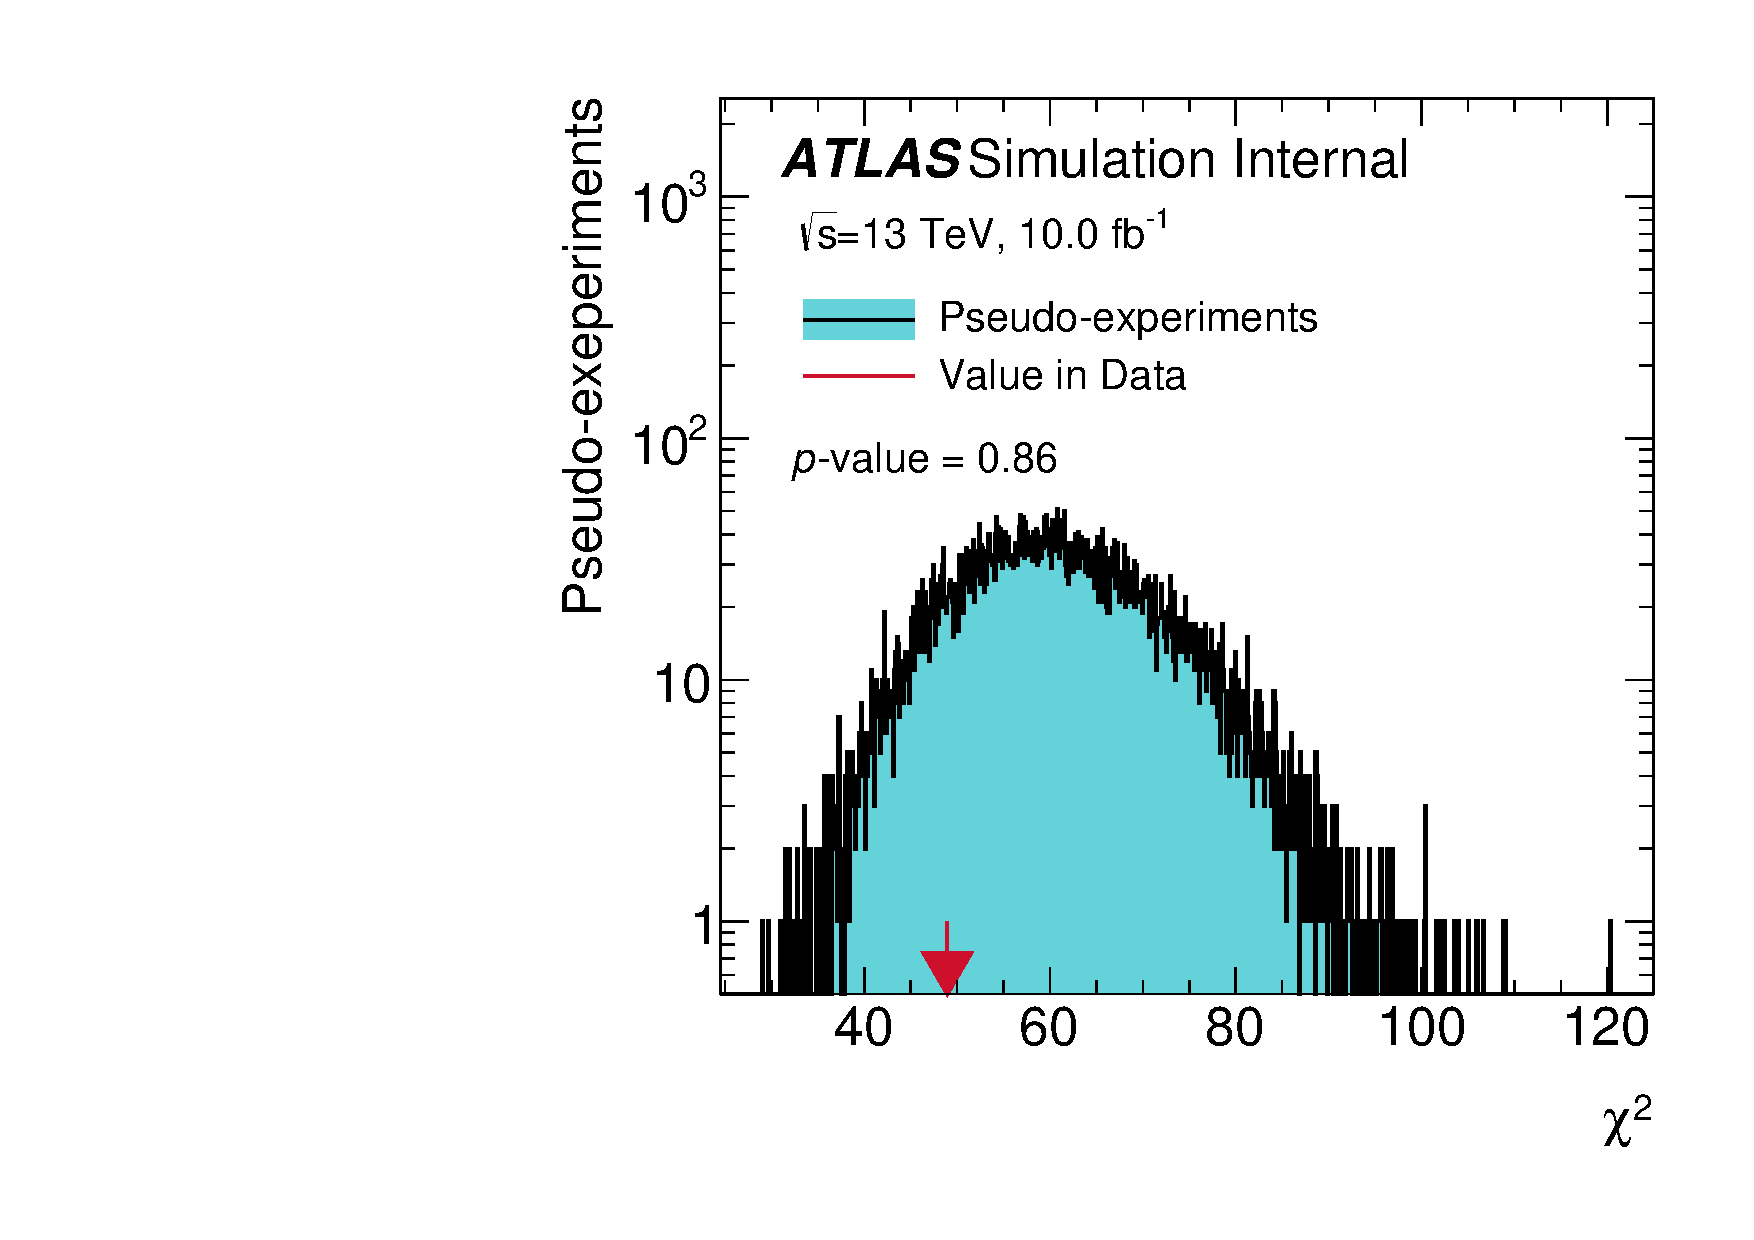
\includegraphics[width=0.47\linewidth, angle=0]{figs/Dibjet/ICHEP/SpuriousSignal/mbj_inc_fix_8585_chi2StatPlot_10fb_v10.pdf}\label{fig:DataLikeChi2StatPlot_bj}}  
%  \end{center}
%  \caption{The distribution of the (a) \bh{} test statistic, (b) \dhunt{} test statistic and (c) $\chi^{2}$ test statistic for 10,000 pseudo experiments
%    compared to the value found in a data-like distribution for the $\geq$1 $b$-tag category.
%  The fraction of pseudo-experiments with a \bh{}, \dhunt{} or $\chi^{2}$ test statistic greater than the value in data is the estimation of the respective \mbox{$p$-value}. }
%  \label{fig:DataLikeStatPlots_bj}
%\end{figure}

However, conclusions cannot be draw from one data-like distribution,
as this does not represent the full range of possible fluctuations that are possible.
Therefore, the search phase is applied to an ensemble of data-like distributions,
each created using a different set of Poisson fluctuations.
Figure~\ref{fig:pValueHists_bb} and Figure~\ref{fig:pValueHists_bj} shows the distribution of
the \bh{}, \dhunt{} and $\chi^{2}$ \mbox{$p$-value}s for 200 different data-like distributions,
for the 2 $b$-tag and $\geq$1 $b$-tag category respectively.
There is no evidence of a fit-bias causing spurious signal in either category,
which could be seen by a bias towards low \bh{} \mbox{$p$-value}s causing fake signals
or a bias toward low \dhunt{} \mbox{$p$-value}s causing fake deficits.
The distribution of the $\chi^{2}$ \mbox{$p$-value}s also indicates that there is good fit quality in both tagging categories.

Hence, it can be concluded that the 3 parameter fit function is a good description of the simulated QCD background
and that there is no evidence that spurious signal can occur.
Similar tests were performed for the 4 parameter fit function but are not presented here because,
as shown in Section~\ref{sec:bkg-summer_global},
the 3 parameter dijet fit function is chosen in both categories for this data-set.

\begin{figure}[!htb]
  \begin{center}
   \captionsetup[subfigure]{aboveskip=0pt,justification=centering}
  \subcaptionbox{\bh{}}{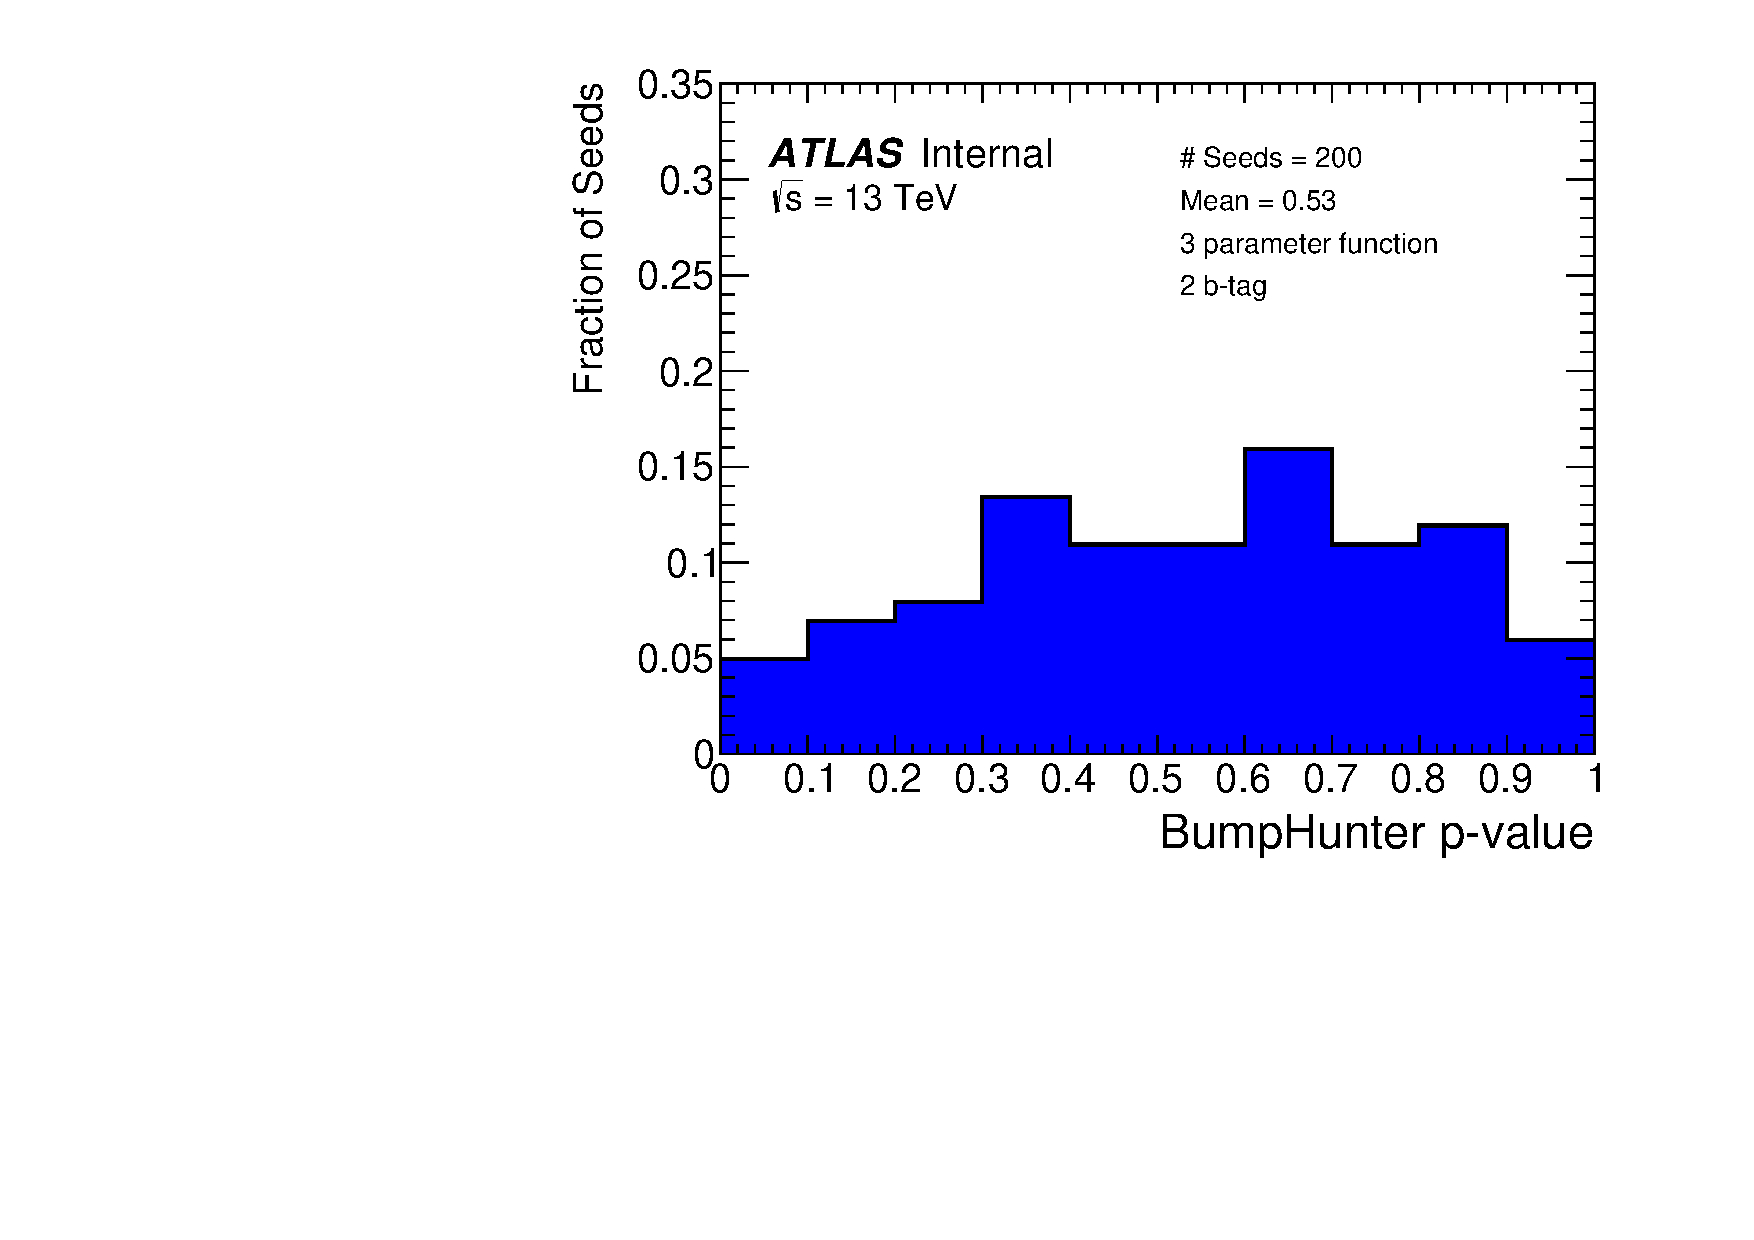
\includegraphics[width=0.4\linewidth, angle=0]{figs/Dibjet/ICHEP/SpuriousSignal/mbb_fix_8585_pValHist_bumpHunter.pdf}}
  \subcaptionbox{\dhunt{}}{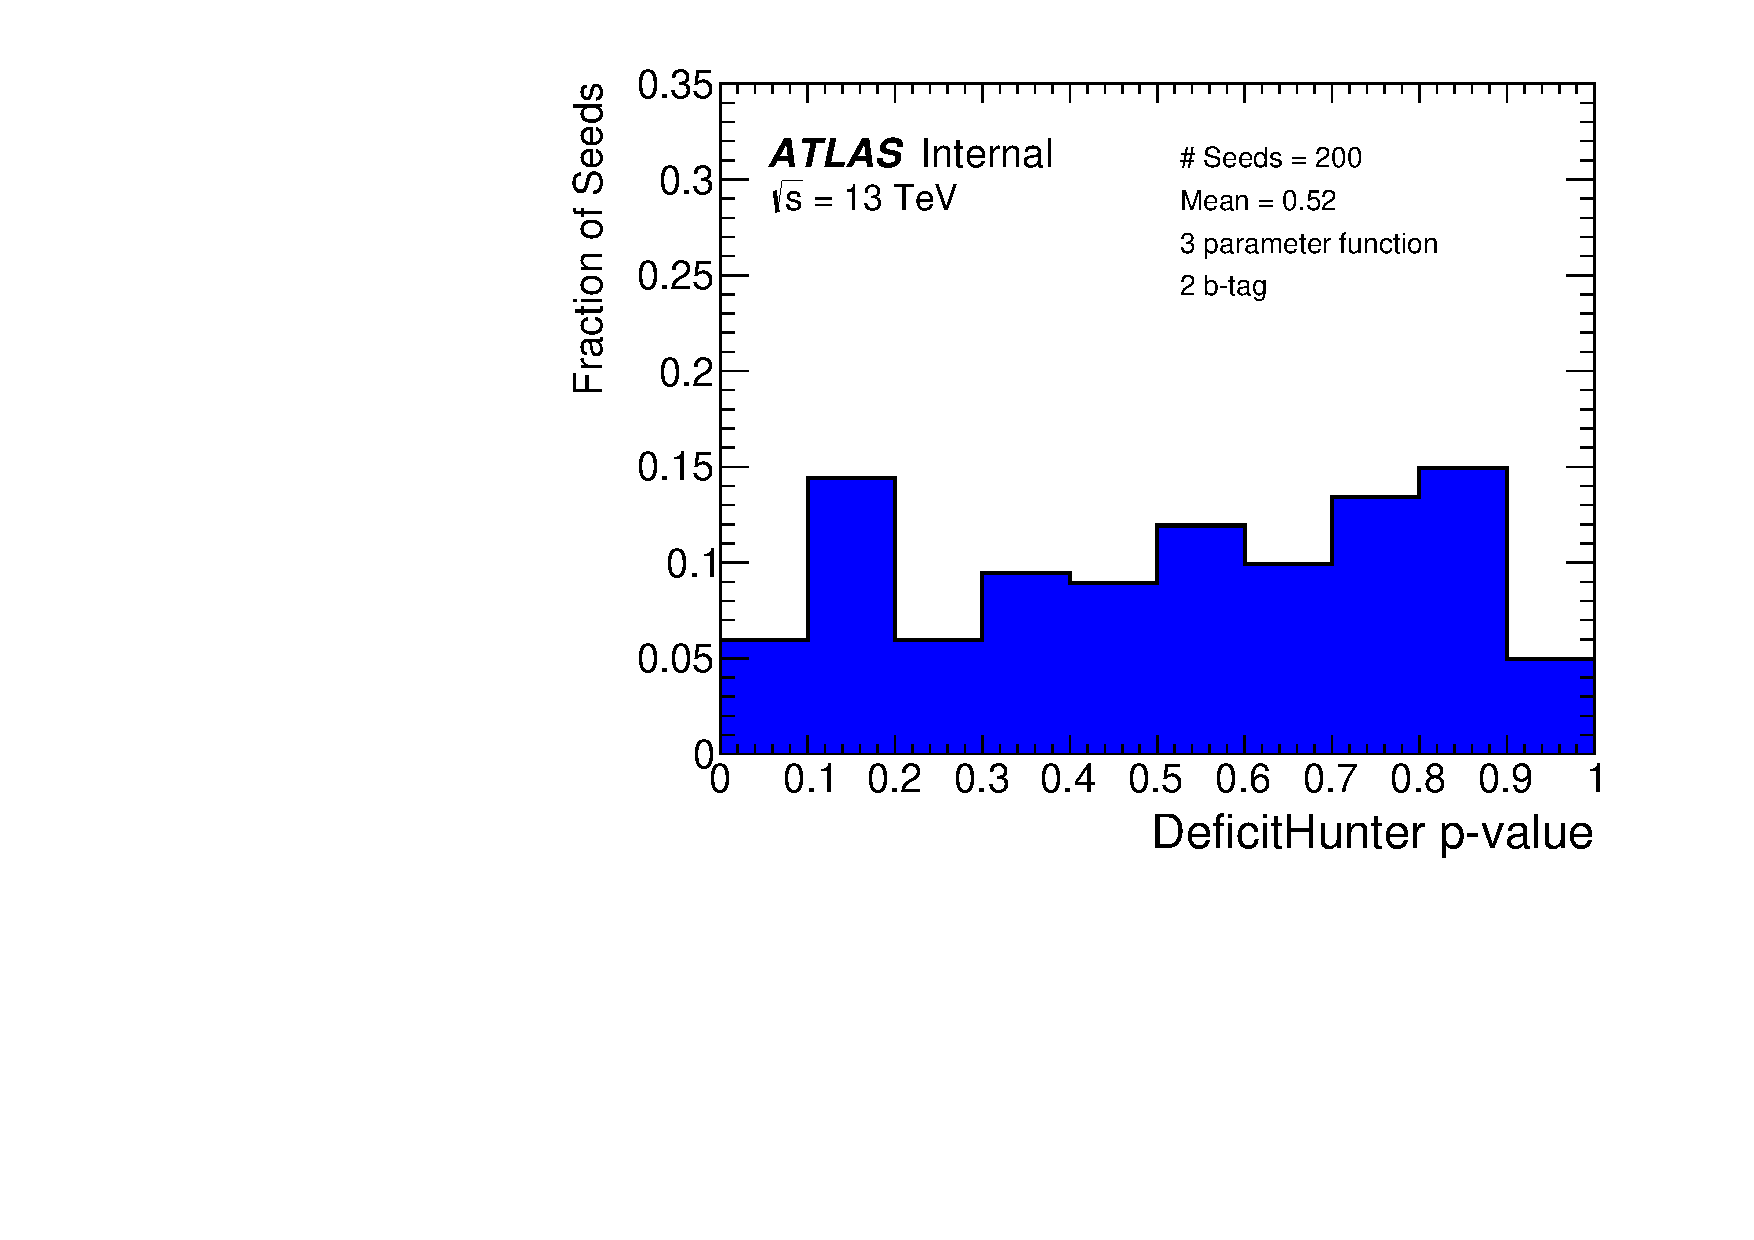
\includegraphics[width=0.4\linewidth, angle=0]{figs/Dibjet/ICHEP/SpuriousSignal/mbb_fix_8585_pValHist_deficitHunter.pdf}}\\
  \subcaptionbox{$\chi^{2}$}{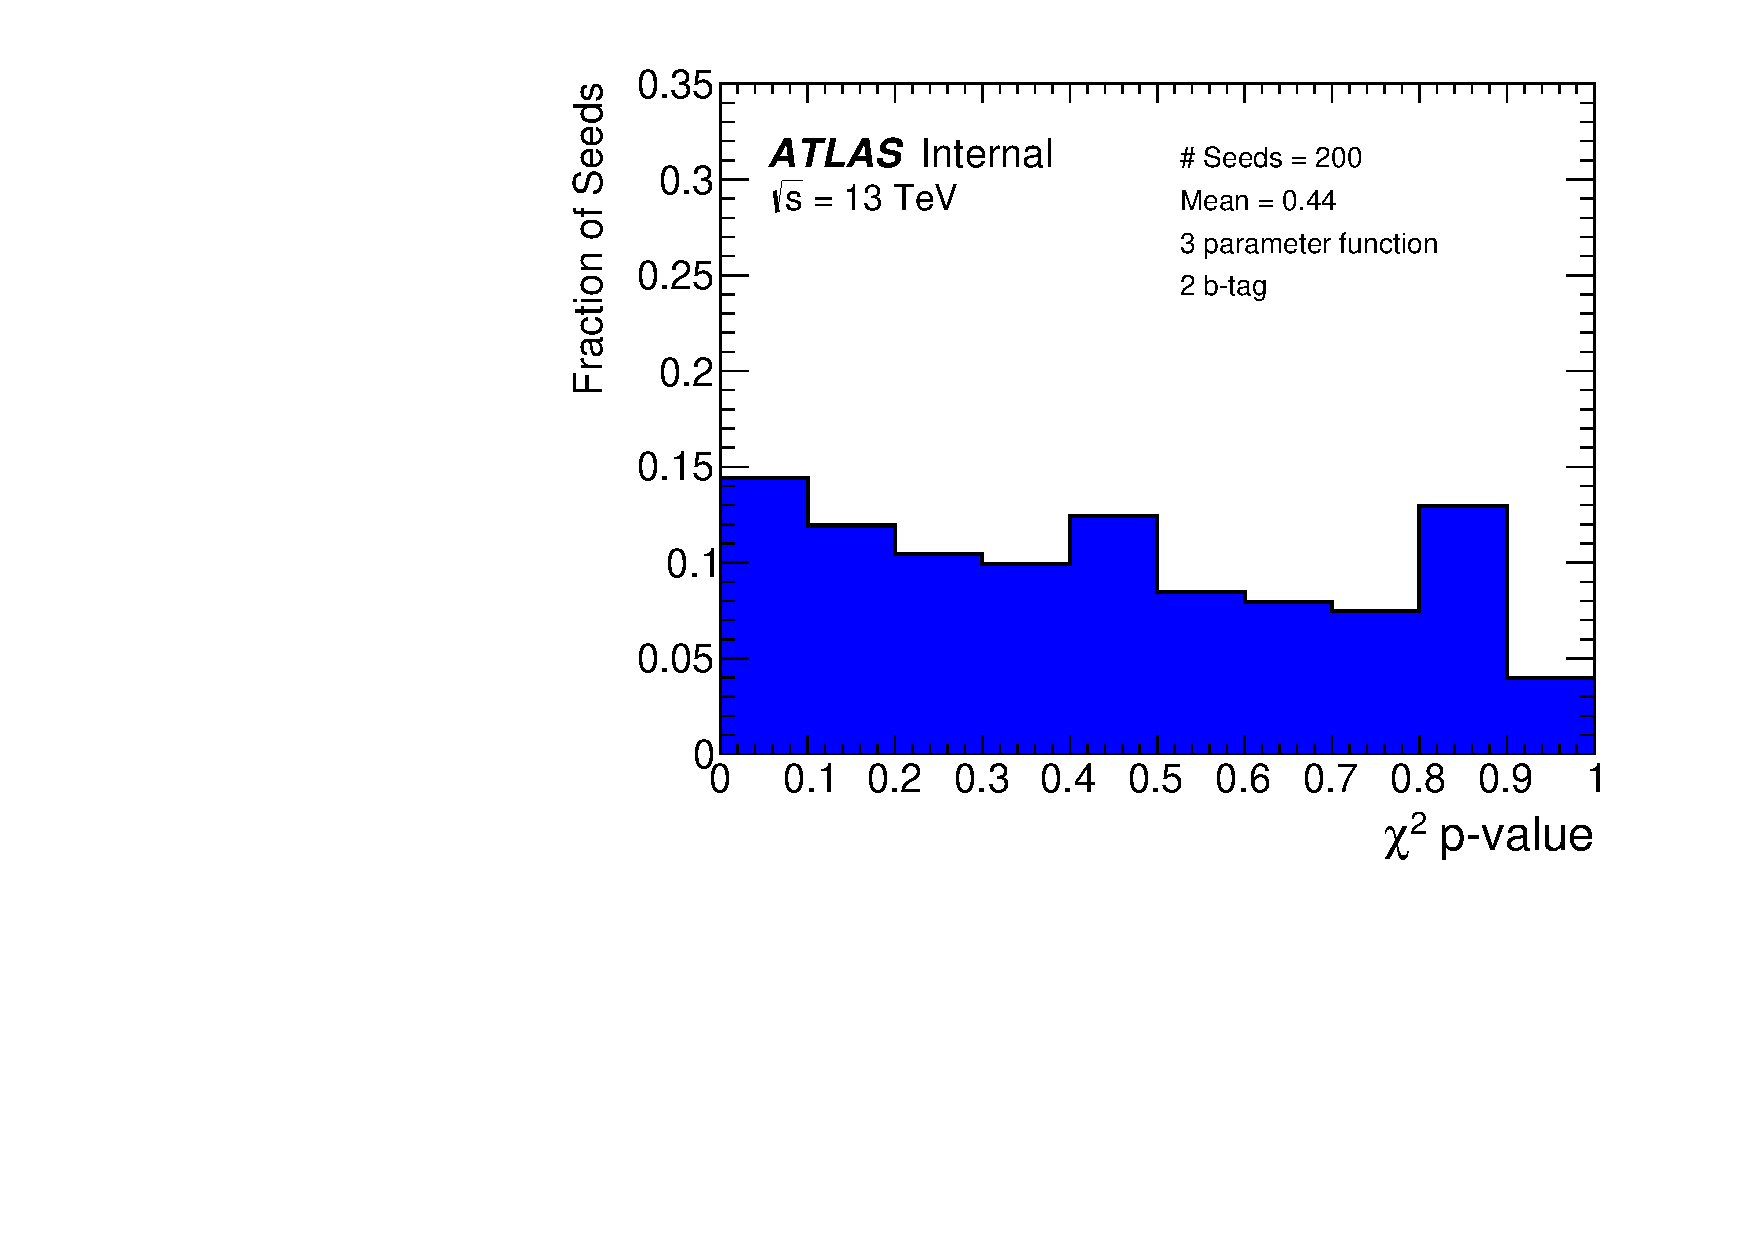
\includegraphics[width=0.4\linewidth, angle=0]{figs/Dibjet/ICHEP/SpuriousSignal/mbb_fix_8585_pValHist_chi2.pdf}}
  \end{center}
  \caption{The distribution of (a) \bh{}, (b) \dhunt{} and (c) $\chi^{2}$ \mbox{$p$-value}s for fits to
    200 data-like dijet mass spectra in the 2 $b$-tag category.
    The \summer{} data-set event selection has been applied.}
  \label{fig:pValueHists_bb}
  \begin{center}
   \captionsetup[subfigure]{aboveskip=0pt,justification=centering}
  \subcaptionbox{\bh{}}{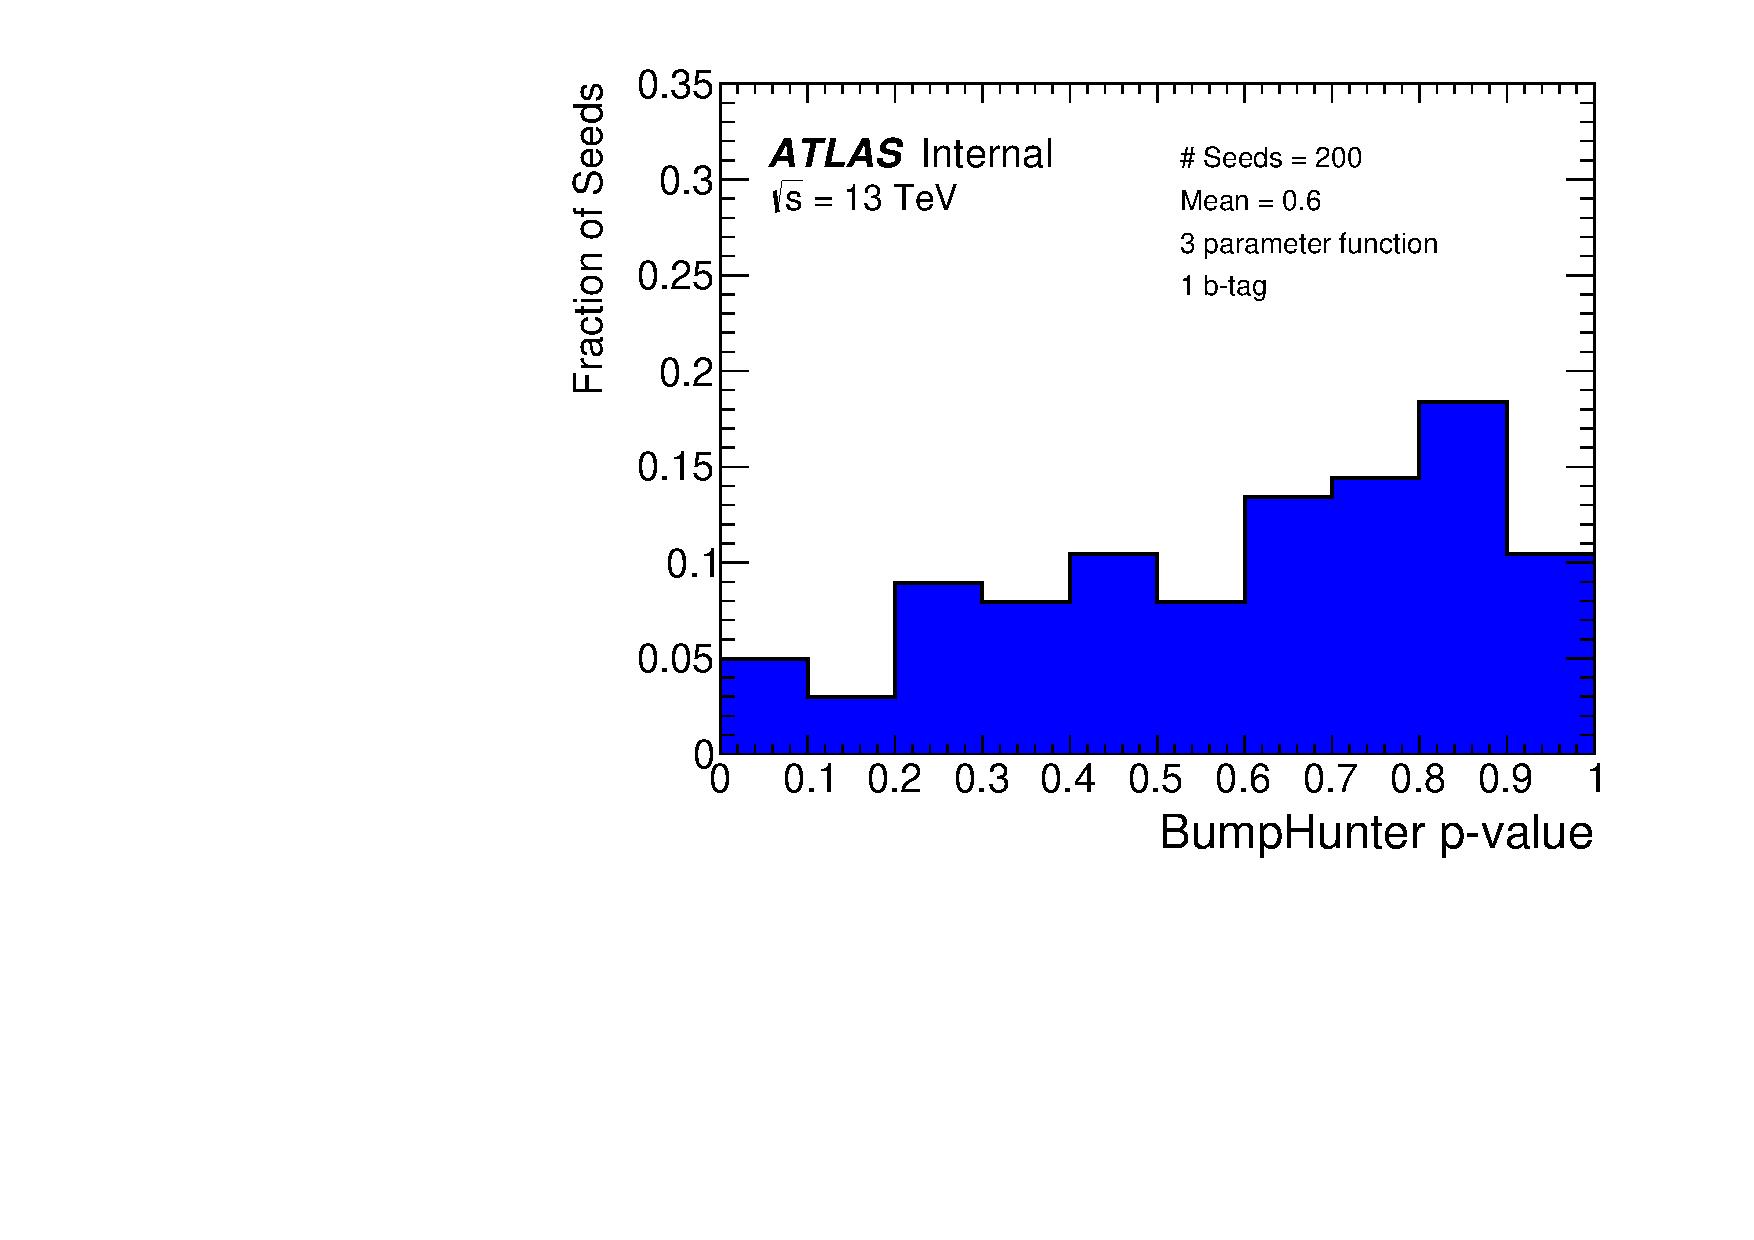
\includegraphics[width=0.4\linewidth, angle=0]{figs/Dibjet/ICHEP/SpuriousSignal/mbj_inc_fix_8585_pValHist_bumpHunter.pdf}}
  \subcaptionbox{\dhunt{}}{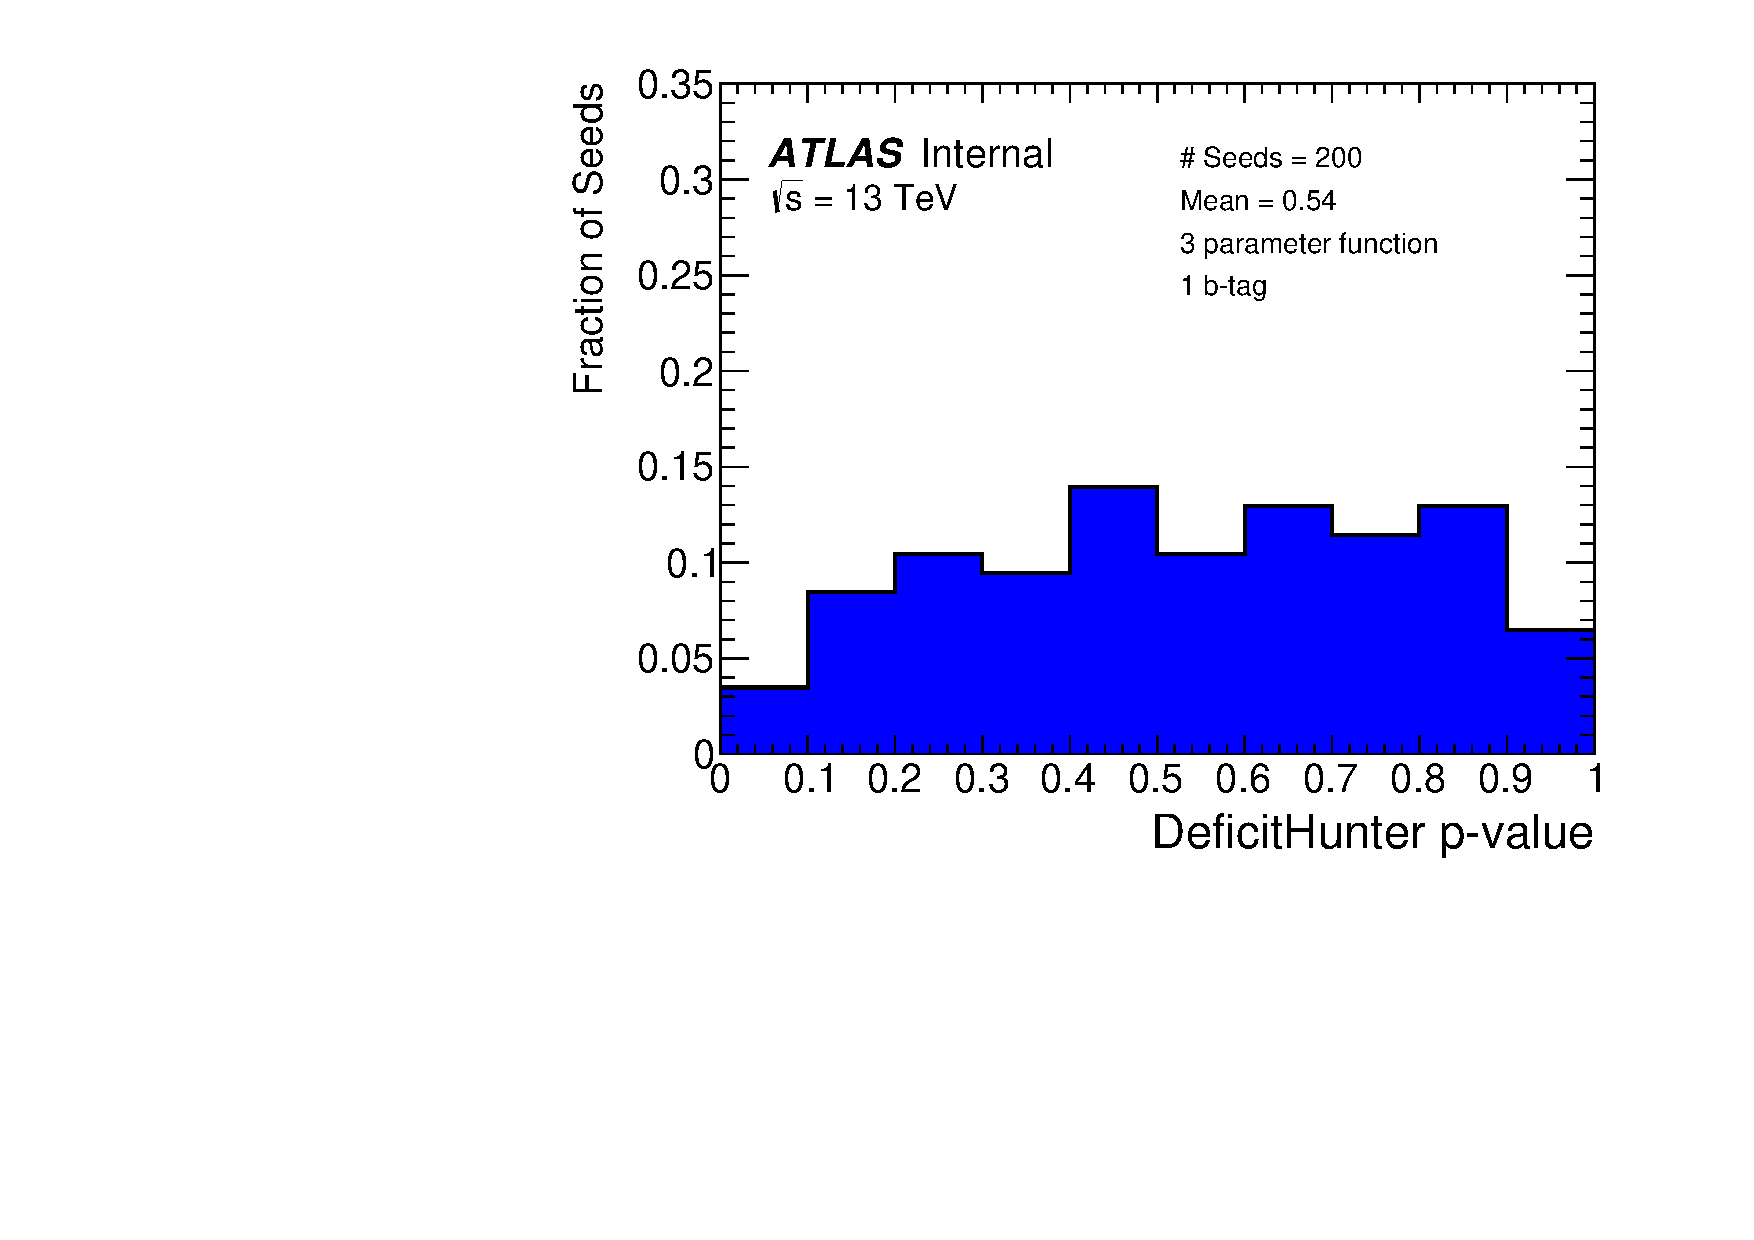
\includegraphics[width=0.4\linewidth, angle=0]{figs/Dibjet/ICHEP/SpuriousSignal/mbj_inc_fix_8585_pValHist_deficitHunter.pdf}}\\
  \subcaptionbox{$\chi^{2}$}{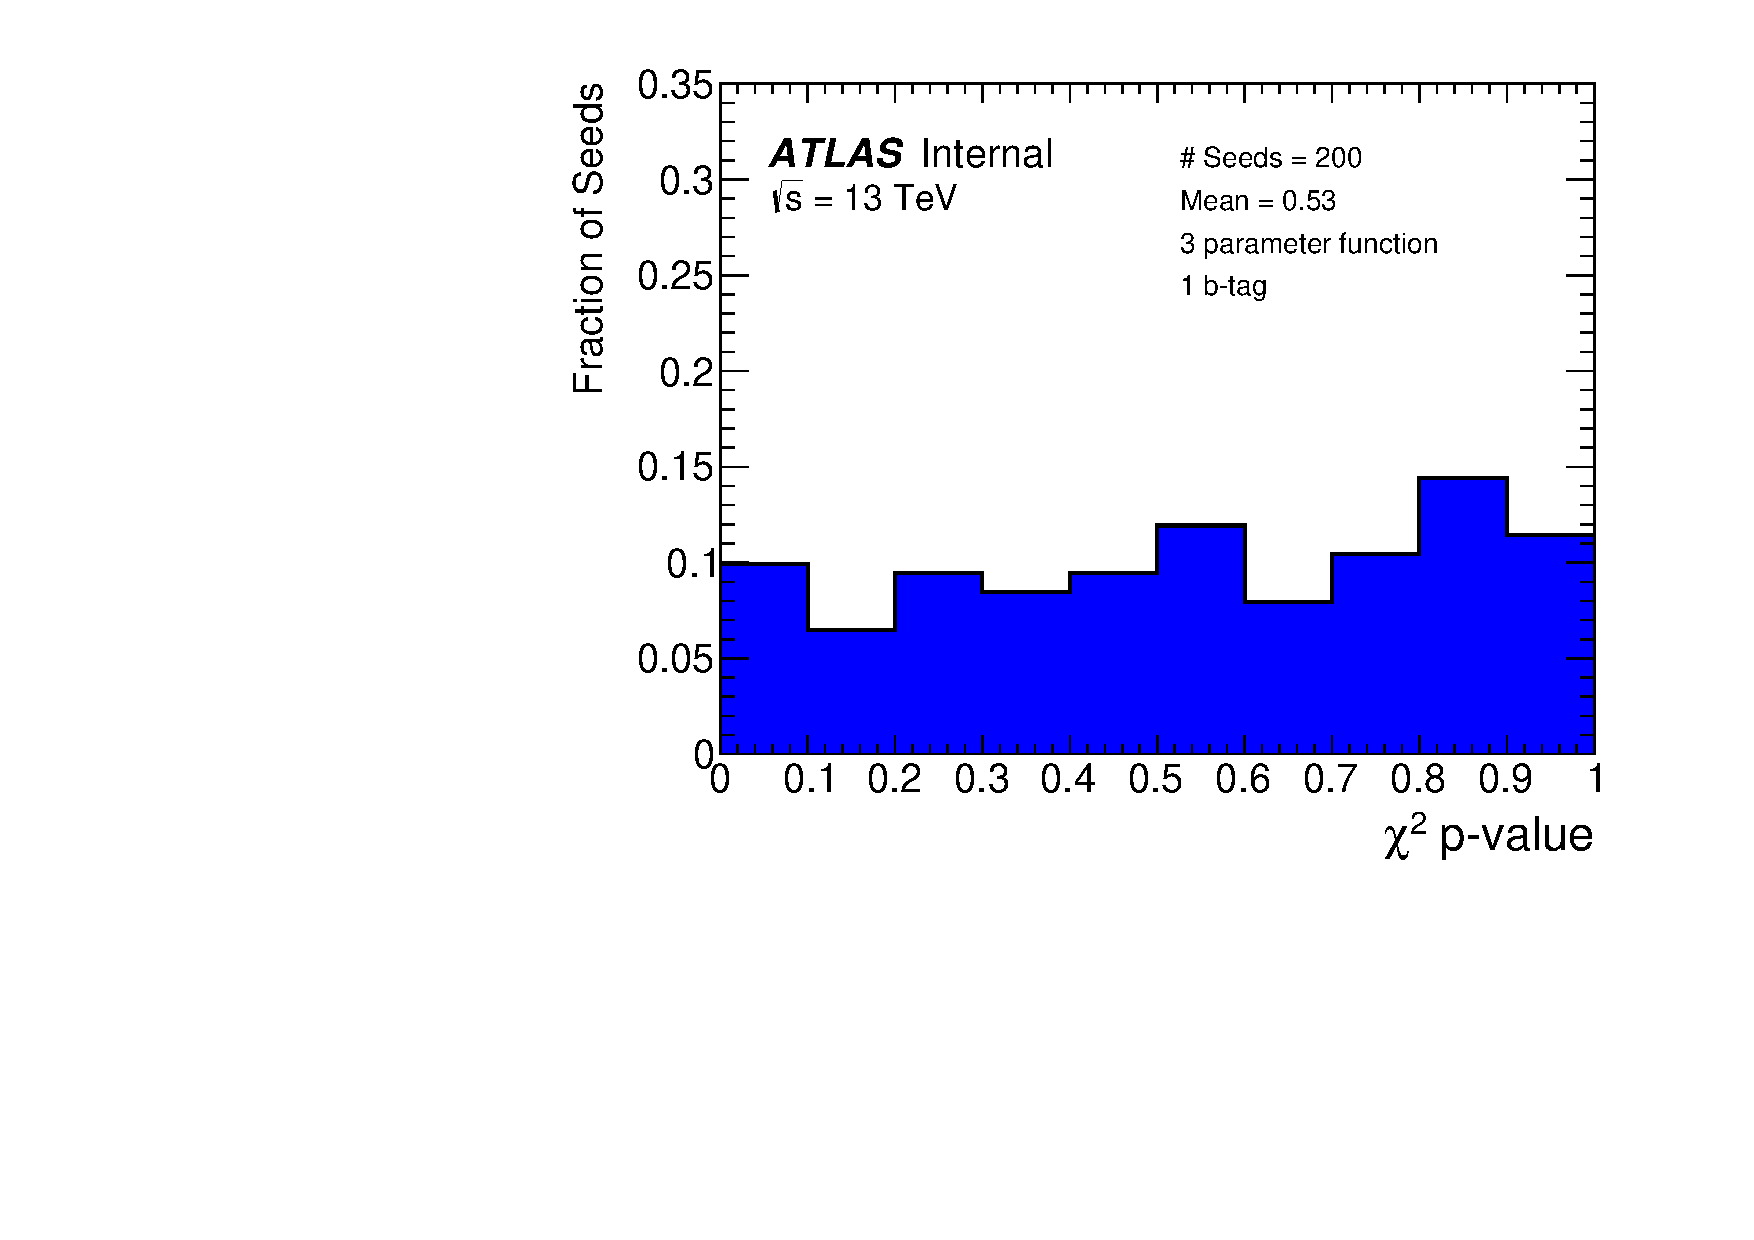
\includegraphics[width=0.4\linewidth, angle=0]{figs/Dibjet/ICHEP/SpuriousSignal/mbj_inc_fix_8585_pValHist_chi2.pdf}}
  \end{center}
  \caption{The distribution of (a) \bh{}, (b) \dhunt{} and (c) $\chi^{2}$ \mbox{$p$-value}s for fits to
    200 data-like dijet mass spectra in the $\geq1$ $b$-tag category.
    The \summer{} data-set event selection has been applied.}
  \label{fig:pValueHists_bj}
\end{figure}


\subsection{Fit Tests: Signal Injection}
\label{sec:bkg-summer_sigInj}

It has been shown in previous iterations of the inclusive dijet and di-$b$-jet searches at ATLAS~\cite{dijet-mori16_paper,dibjet-mori16_paper}
that the 3 parameter dijet fit function is able to describe a simulated QCD background when a signal has been injected.
This is because the parameters of the 3 parameter dijet fit function are highly constrained by the QCD background,
and as such significant fit biases cannot occur when signal is introduced.
Hence, it is concluded the background estimation from a 3 parameter dijet fit function is robust against the presence of signal.

\FloatBarrier

\subsection{Results}
\label{sec:bkg-summer_results}

It has been shown that the 3 parameter dijet fit function has a
sufficient number of parameters to provide an adequate background
description in both $b$-tagging categories in the fit region that has been chosen
and that there is no evidence that spurious signal can occur.
Hence, for the \summer{} data-set the 3 parameter fit function
provides a valid background estimation in both categories.

Figure~\ref{fig:bkg-summer_searchPhase} shows the final
\summer{} data-set and the background estimate using the 3 parameter dijet fit function
in the 2 and $\geq1$ $b$-tag categories.
The upper panel shows the data compared to the background fit,
in addition the benchmark signal models with enhanced cross sections have been overlaid.
The lower panel shows the significance of the difference between the data and background estimate.


\begin{figure}[!htb]
  \begin{center}
    \captionsetup[subfigure]{aboveskip=0pt,justification=centering}
   \subcaptionbox{2 $b$-tag}{\includegraphics[width=0.47\linewidth, angle=0]{figs/Dibjet/ICHEP/bkg-SearchPhase_bb.pdf}}
   \subcaptionbox{$\geq$1 $b$-tag}{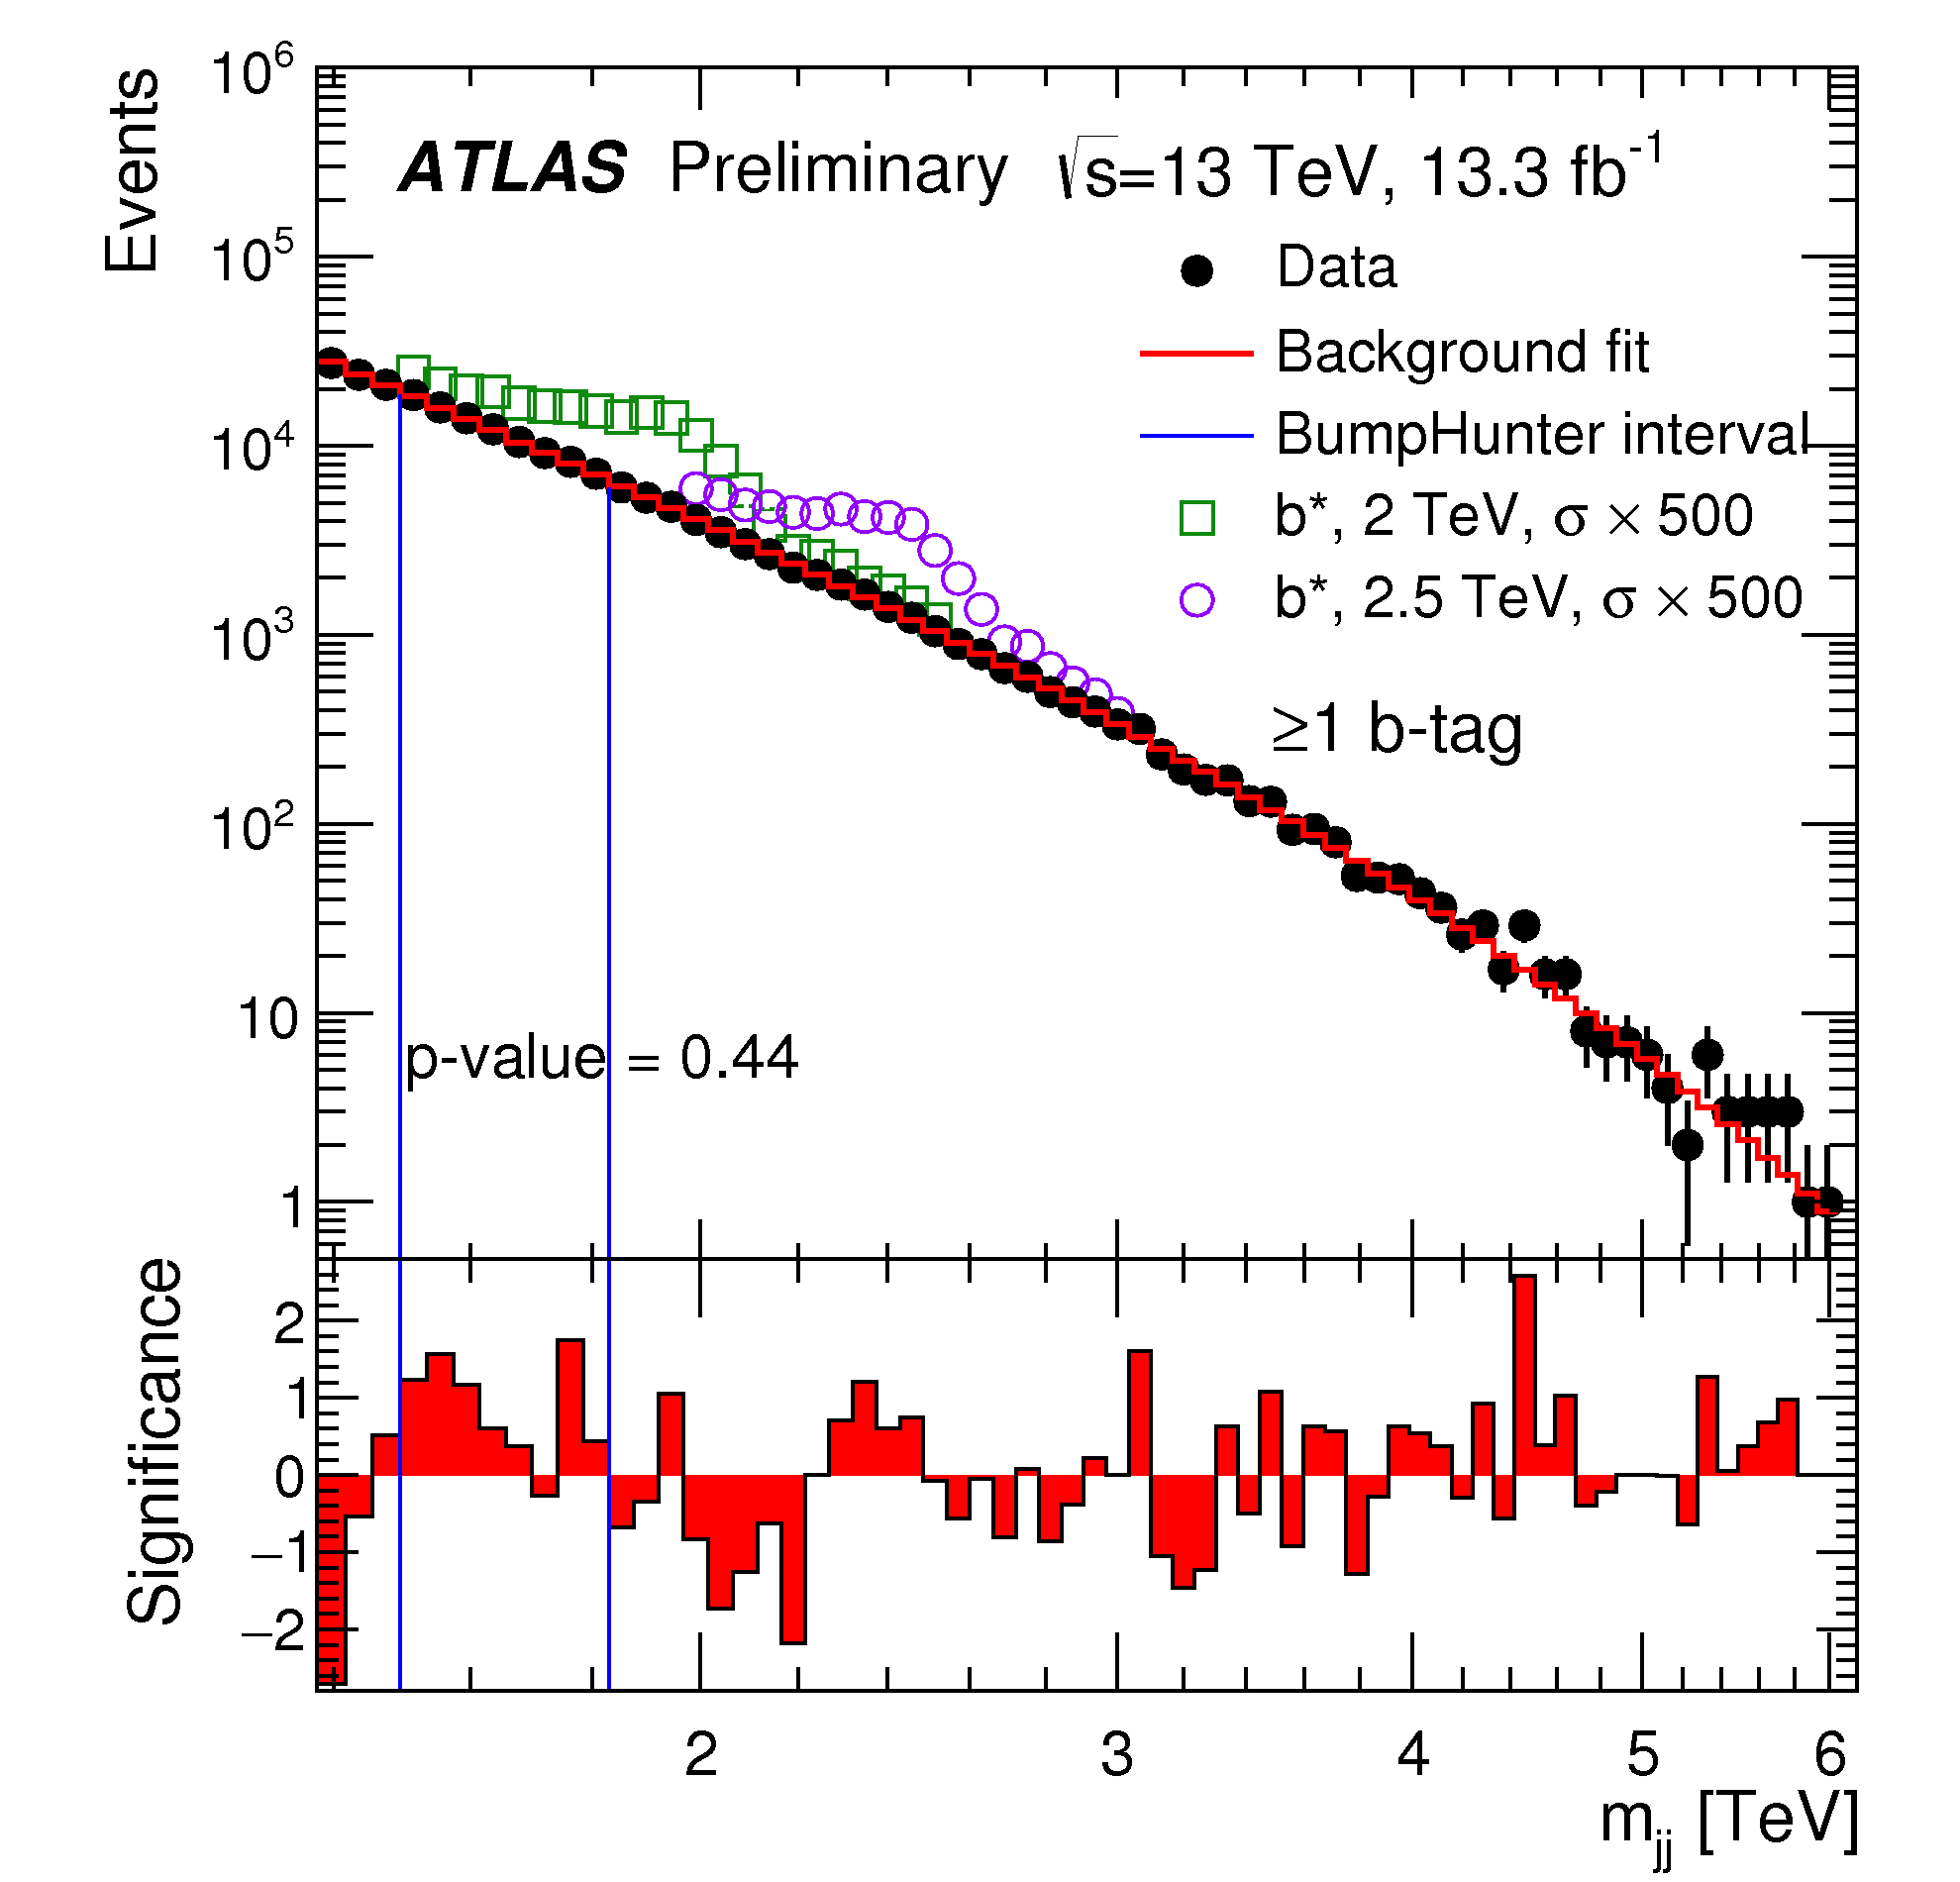
\includegraphics[width=0.47\linewidth, angle=0]{figs/Dibjet/ICHEP/bkg-SearchPhase_b.pdf}}
  \end{center}
  \caption[The final \summer{} data-set in the (a) 2 $b$-tag and the (b) $\geq$1 $b$-tag category,
            where the background has been modelled using the 3 parameter dijet fit function.
            The upper panel shows the data compared to the background estimate,
            benchmark signal models with enhanced cross sections are overlaid.
            The lower panel shows the significance of the difference between the data and the background estimate.
            The most discrepant excess as found by the \bh{} algorithm is indicated by the vertical blue lines and the \mbox{$p$-value} of this excess is printed on the plot.]
          {The final \summer{} data-set in the (a) 2 $b$-tag and the (b) $\geq$1 $b$-tag category,
            where the background has been modelled using the 3 parameter dijet fit function.
            The upper panel shows the data compared to the background estimate,
            benchmark signal models with enhanced cross sections are overlaid.
            The lower panel shows the significance of the difference between the data and the background estimate.
            The most discrepant excess as found by the \bh{} algorithm is indicated by the vertical blue lines and the \mbox{$p$-value} of this excess is printed on the plot
            ~\cite{dibjet-ichep_conf}.
          }
  \label{fig:bkg-summer_searchPhase}
\end{figure}

In both cases the \bh{} algorithm has identified the most discrepant excess indicated
in the figure using vertical blue lines.
The \bh{} \mbox{$p$-value} has been calculated using 10,000 pseudo-experiments.
The \bh{} \mbox{$p$-value} is 0.60 in the 2 $b$-tag category
and 0.44 in the $\geq1$ $b$-tag category.
Therefore, it can be concluded that no significant excess is found in either $b$-tag category
and that there is no evidence of new physics in the \summer{} data-set.
As no significant excess is found, limits are set using the \summer{} data-set on the benchmark signal models,
which will be described in Chapter~\ref{sec:lim}.

\section{\lm{} Search Phase}
\label{sec:bkg-full}

This section presents the search phase for the \lm{} data-set.
Section~\ref{sec:bkg-full_stat:bkgsample} describes the background-only samples used for the studies,
Section~\ref{sec:bkg-full_globalFit} describes the studies using the global fit strategy and
Section~\ref{sec:bkg-full_swift} introduces an alternative background modelling strategy called the Sliding Window Fit (SWiFt),
which has been developed and validated in the inclusive dijet analysis on the full 2015+2016 data-set at ATLAS~\cite{dijet-mori17_paper}.
Sections~\ref{sec:bkg-full_windowSel}-\ref{sec:bkg-full_signalInj} shows studies performed to validate the SWiFt background estimation.
Section~\ref{sec:bkg-full_bkg-full_results} presents the results of the search phase full \lm{} data-set.

\subsection{Background-Only Samples}
\label{sec:bkg-full_stat:bkgsample}

The background estimation strategy is tested and developed without using the final data-set, which is known as `blinding'.
Blinding is required such that no bias from the final data-set is introduced into the background estimation strategy.
To perform blinded tests a dijet mass spectrum that is representative of the background is required.
Ideally, Monte-Carlo simulation would be used as was done for the \summer{}
data-set analysis as described in Section~\ref{sec:bkg-full_bkg-summer_fitCR}.
However, for the \lm{} data-set considered Monte-Carlo simulation cannot be produced with a large enough statistical
precision to perform an adequate test of the background estimation strategy.
Instead two fitting test data-sets are used:
a 3 \ifb{} subset of the final test data and a high precision fitting control region.

To create the 3 \ifb{} subset of data,
events are randomly drawn from the final data spectrum as shown in Figure~\ref{fig:fittingDataSubset}.
The dijet mass spectrum of the subset of data represents the shape of the dijet mass spectrum in final data-set,
except with a lower statistical precision.
The luminosity of the subset of data was chosen to be similar to that of a
previous low mass di-$b$-jet search in a similar mass range~\cite{dibjet-lhcp_conf},
such that this subset of data is known not to be sensitive to signal.

\begin{figure}[!htb]
\captionsetup[subfigure]{aboveskip=0pt,justification=centering}
\centering
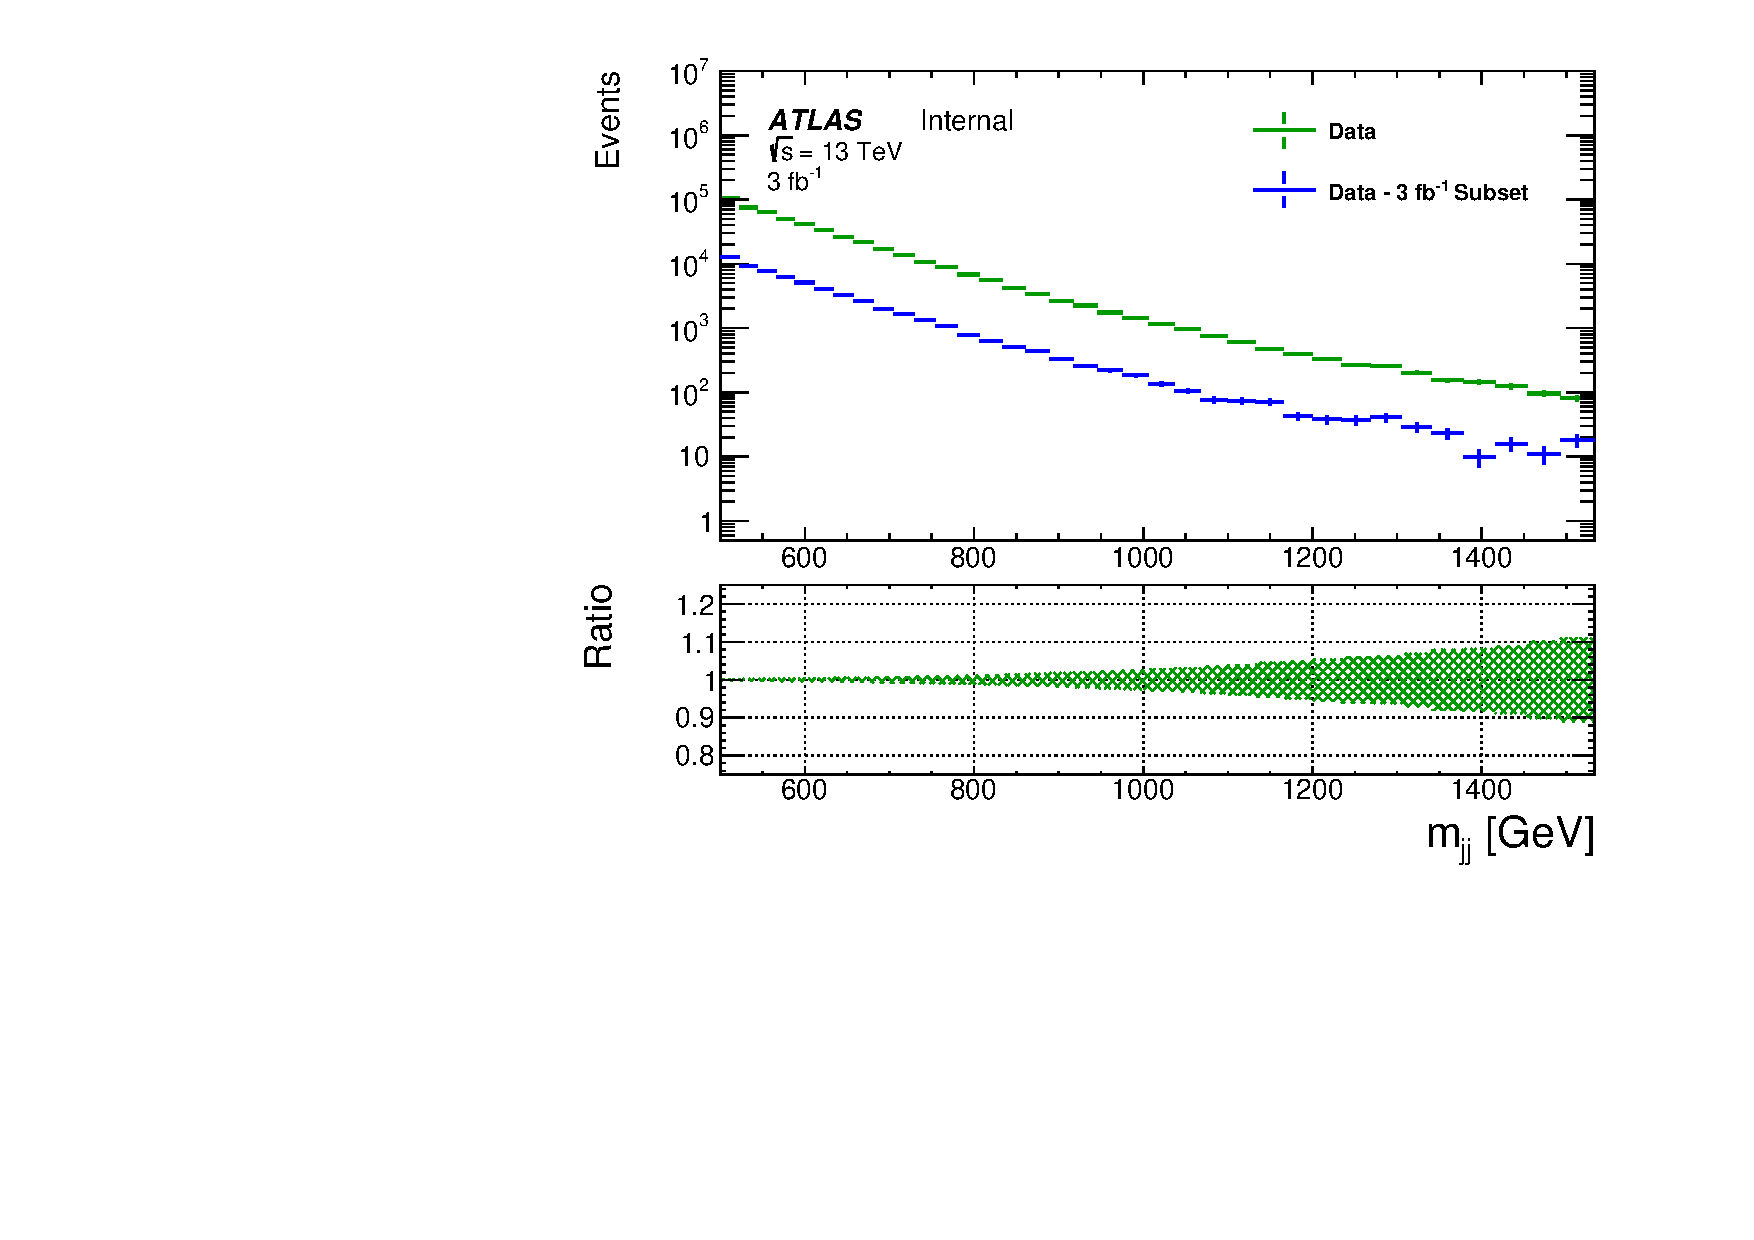
\includegraphics[width=0.7\linewidth, angle=0]{figs/Dibjet/LowMass/FitStudy/subset_dataComp.pdf}
\caption{\label{fig:fittingDataSubset}
  The dijet mass (\mjj{}) spectra of the full \lm{} data-set and a 3 \ifb{} subset of \lm{} data.
  The lower panel shows a a ratio.}
\end{figure}

To derive the fitting control region for the \lm{} data-set,
two dijet mass spectra from data are used as inputs.
The first is the dijet mass spectrum of the~3 \ifb{} subset described above.
The second is the dijet mass spectrum of events that have passed the \lm{} event-selection
except that no offline $b$-tagging selection is applied, this is referred to as the 0-tag dijet mass spectrum.
Figure~\ref{fig:fittingCR}(a) shows a comparison of the dijet mass spectrum of the 0-tag data and the 3 \ifb{} data subset.

\begin{figure}[!htb]
\captionsetup[subfigure]{aboveskip=0pt,justification=centering}
\centering
\hspace{-2mm}
\subcaptionbox{0-tag data and a 3 \ifb{}\\subset of 2-tag data} {
  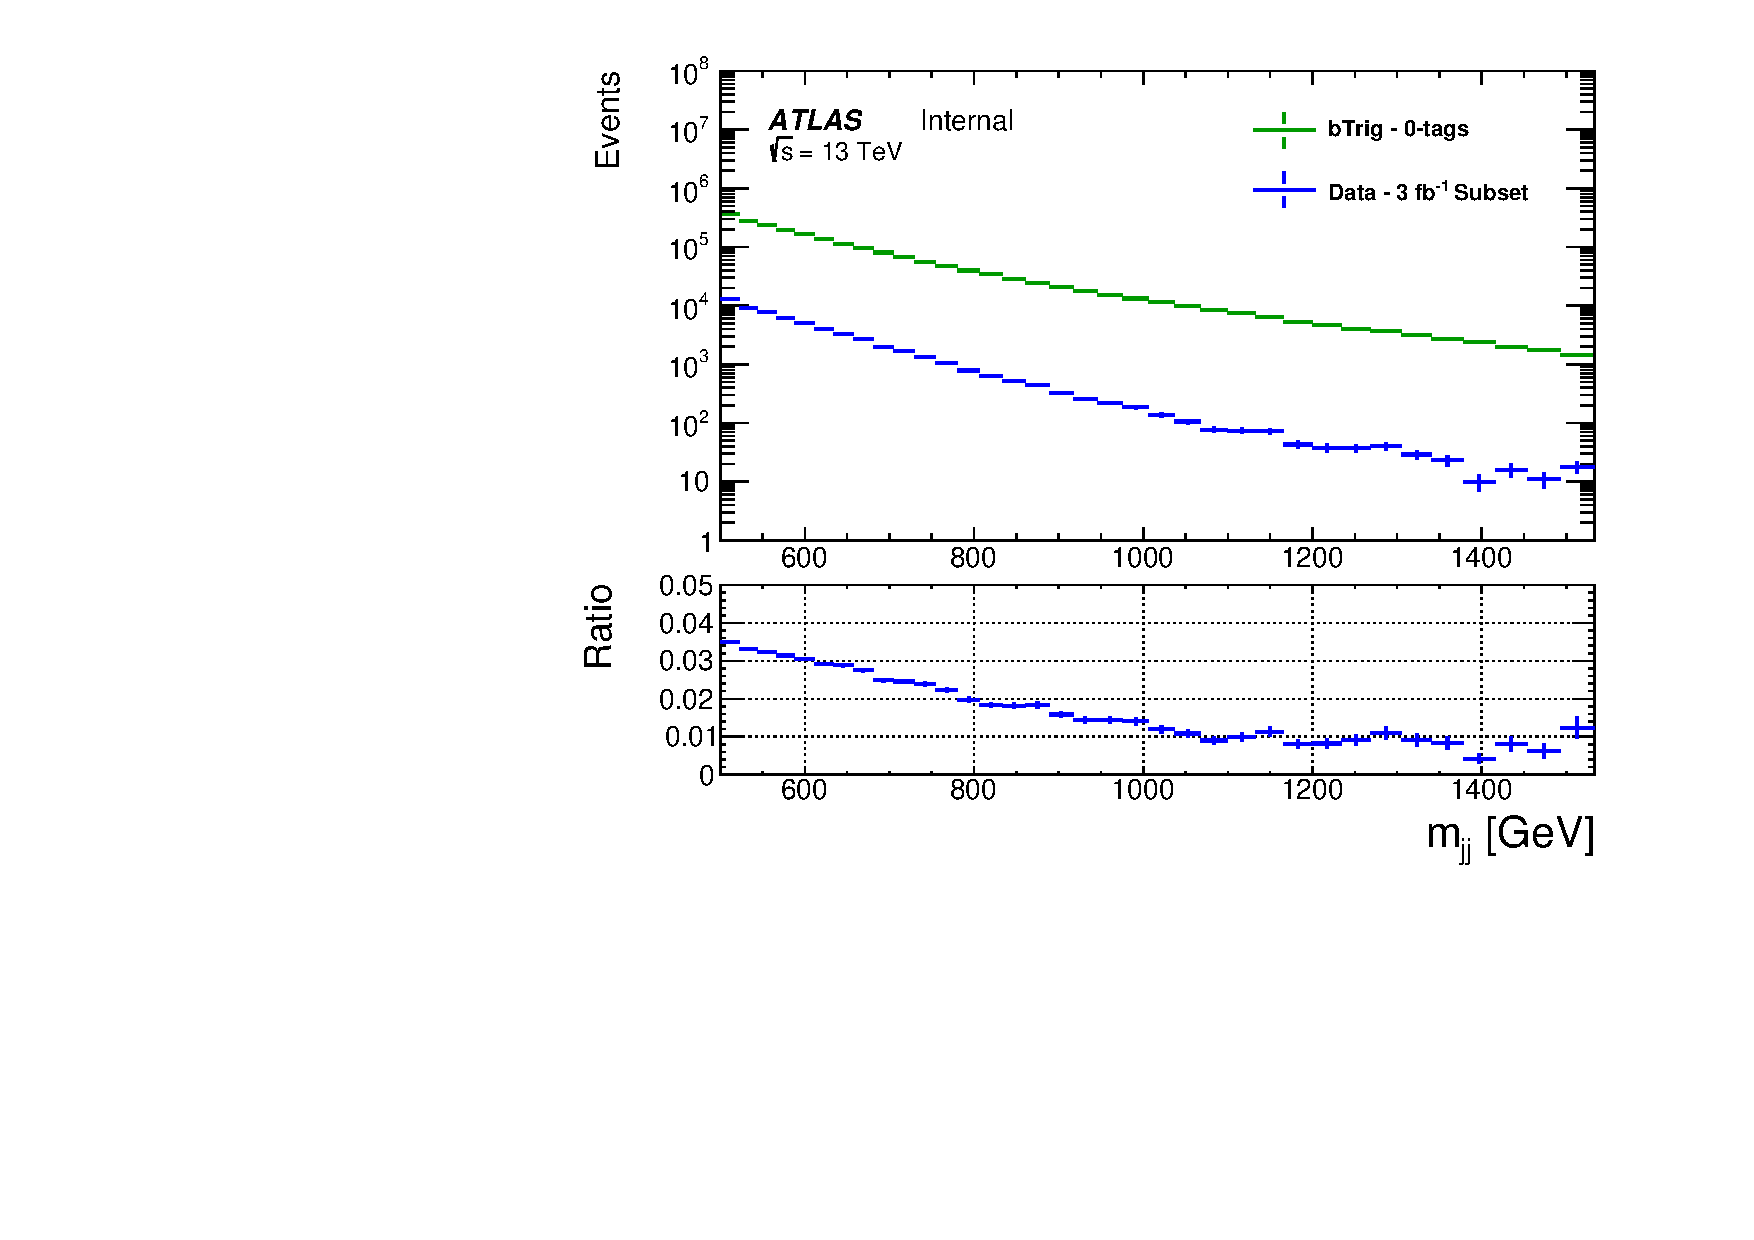
\includegraphics[width=0.51\linewidth, angle=0]{figs/Dibjet/LowMass/FitStudy/corrFitCR_0tag_subset.pdf}
}\hspace{-8mm}
\subcaptionbox{Offline tagging efficiency\\w.r.t. online tagging.} {
  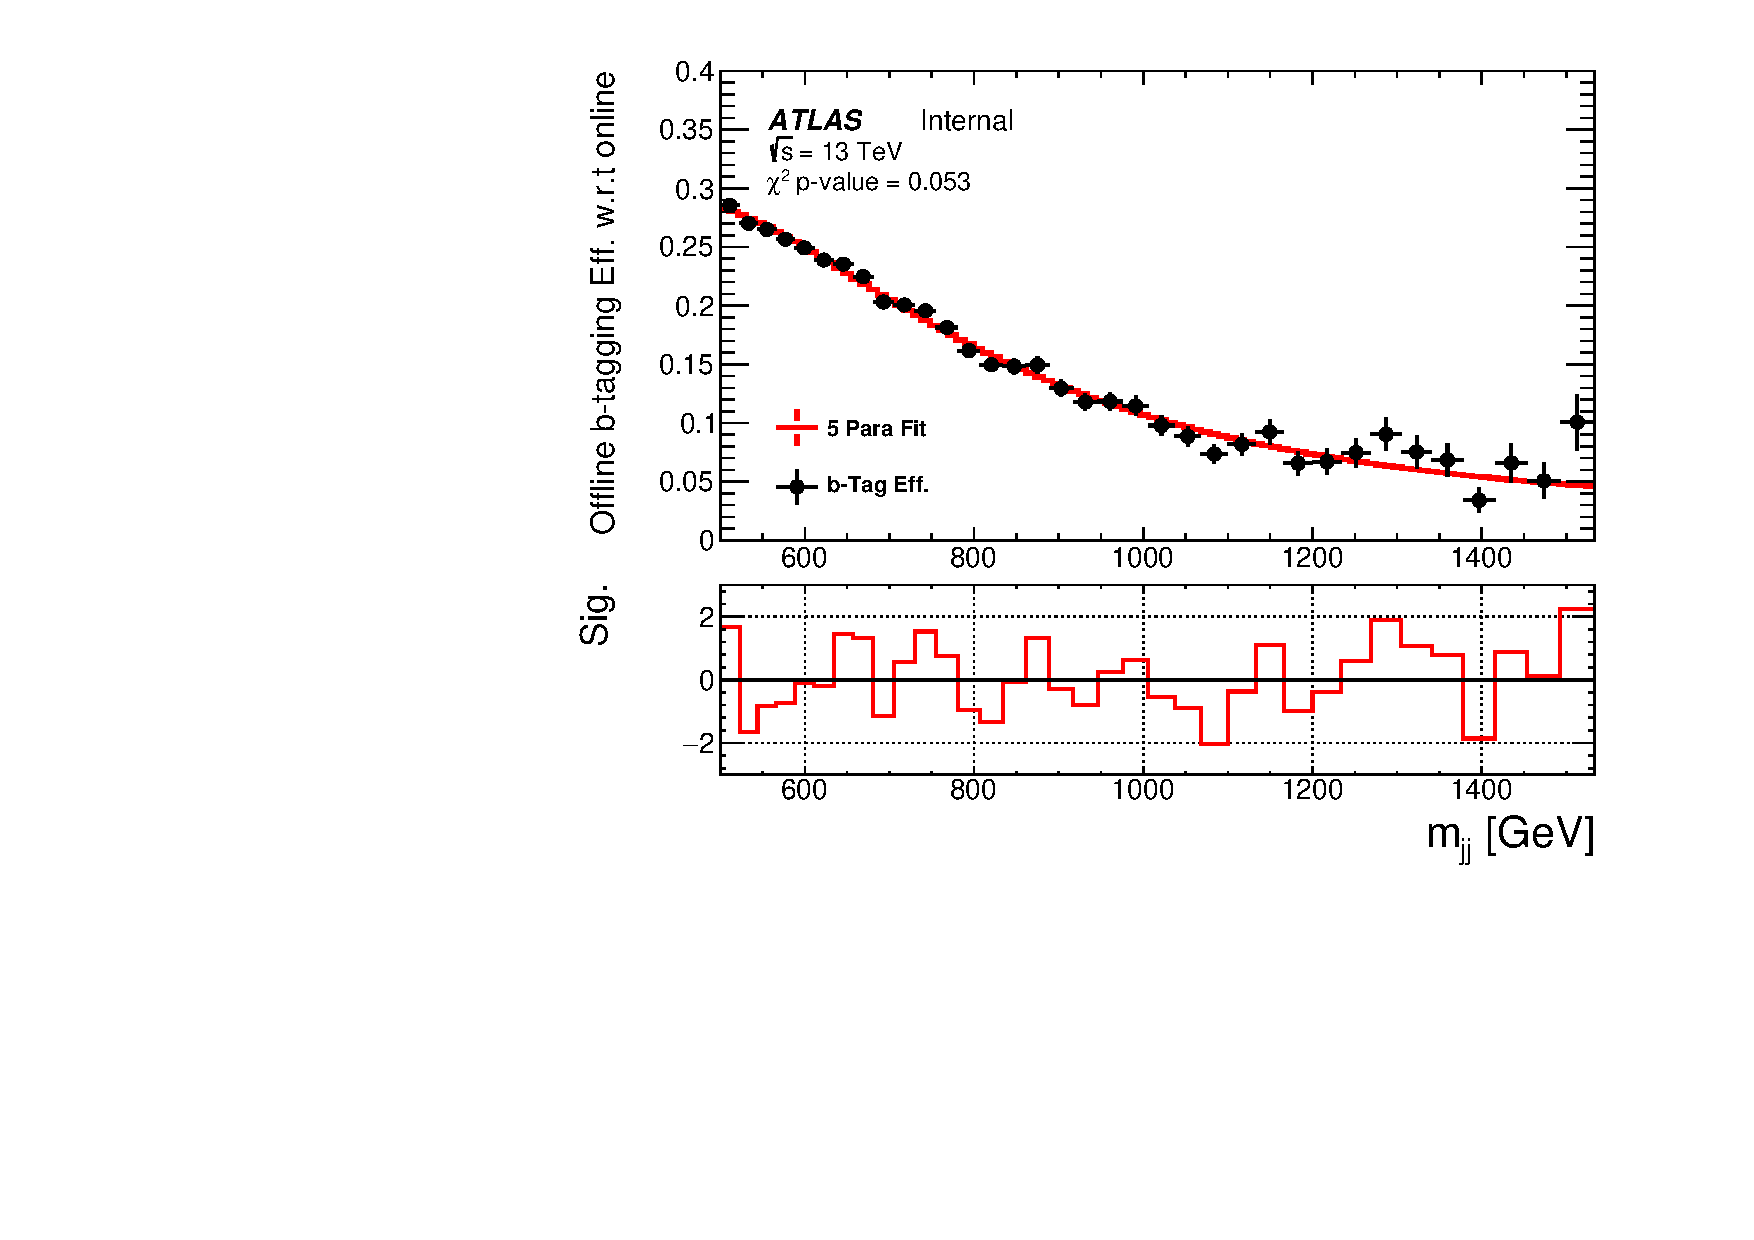
\includegraphics[width=0.51\linewidth, angle=0]{figs/Dibjet/LowMass/FitStudy/corrFitCR_5parFit.pdf}
} \hspace{-2mm} \\
\hspace{-2mm}
\subcaptionbox{The fitting CR and\\the 2-tag data.} {
  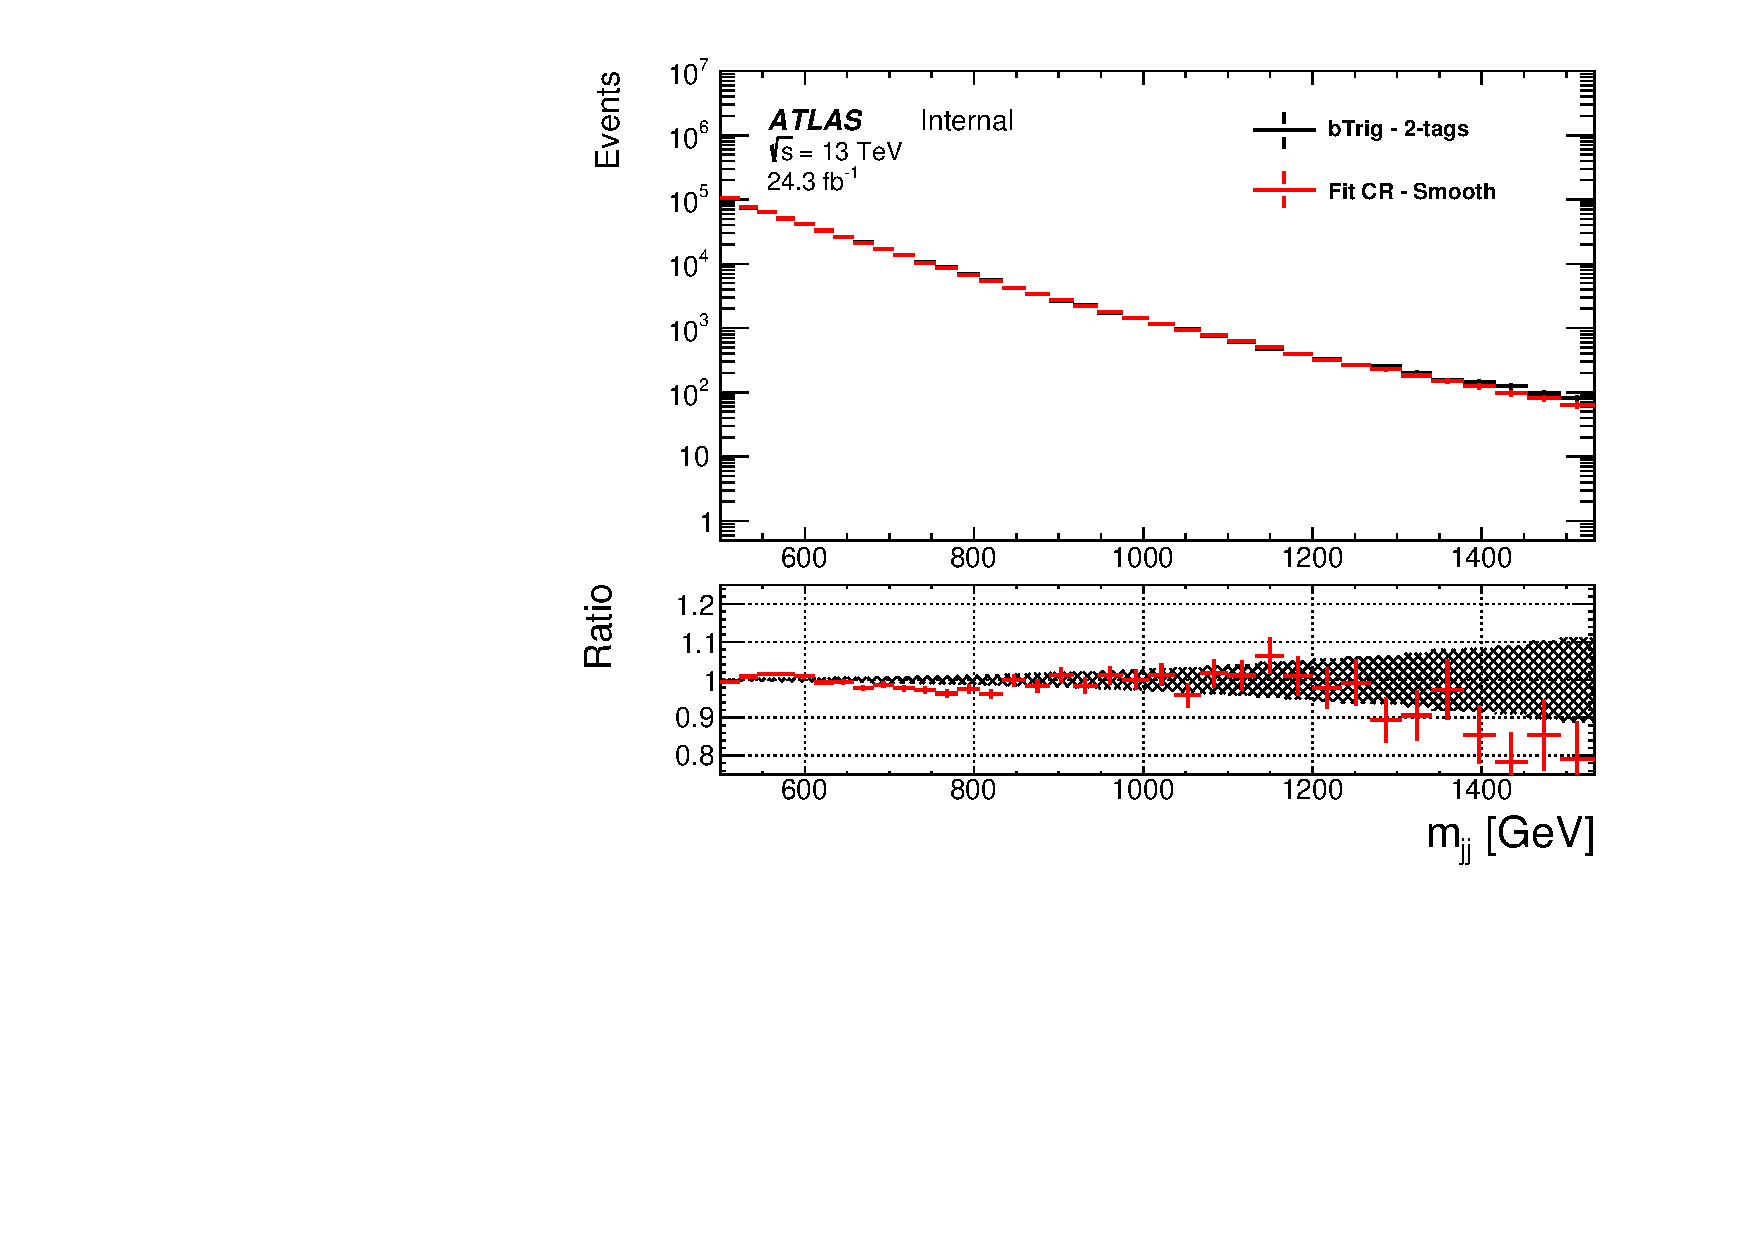
\includegraphics[width=0.51\linewidth, angle=0]{figs/Dibjet/LowMass/FitStudy/corrFitCR_dataComp.pdf}
}\hspace{-8mm}
\subcaptionbox{Smooth and data-like fitting \\control region distributions} {
  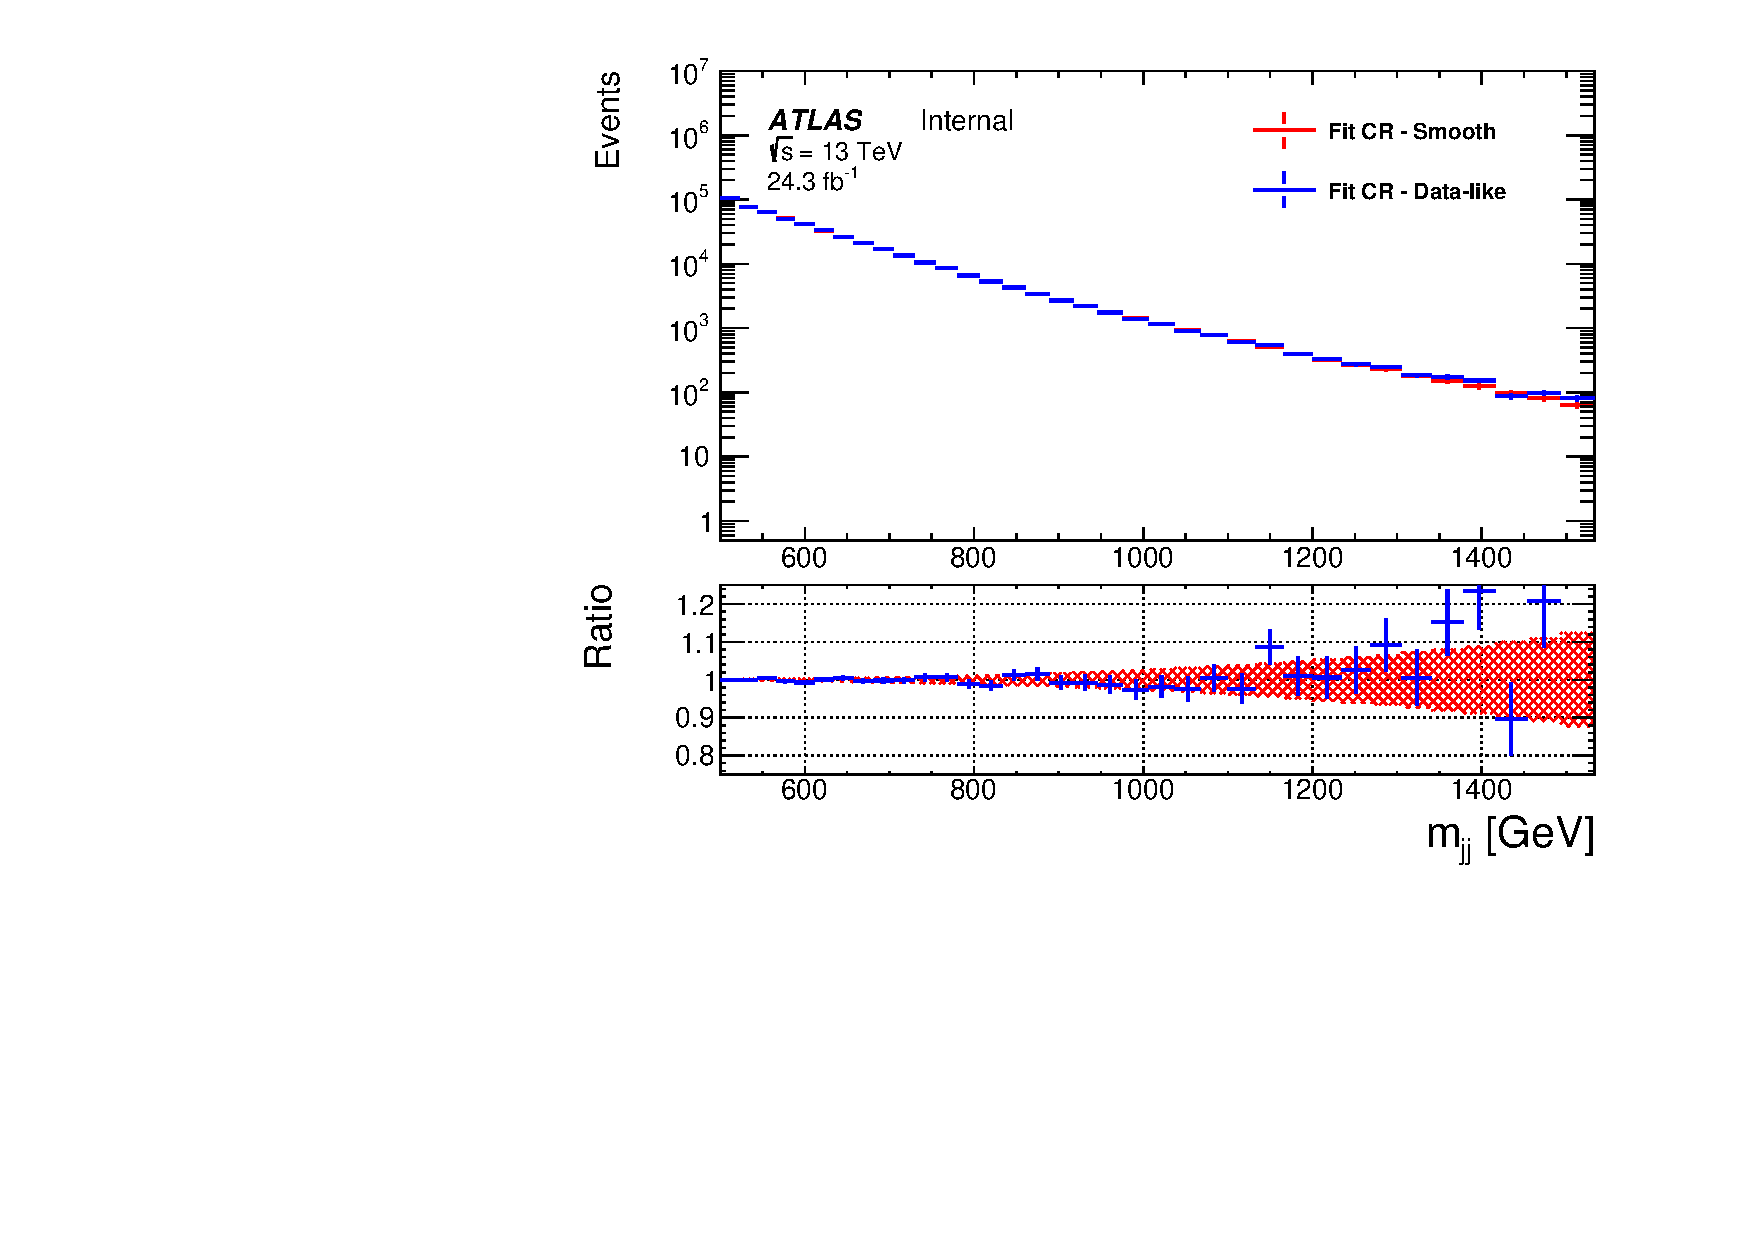
\includegraphics[width=0.51\linewidth, angle=0]{figs/Dibjet/LowMass/FitStudy/corrFitCR_smooth_dataLike.pdf}
}
\hspace{-2mm}

\caption{\label{fig:fittingCR}
  A figure showing the process of obtaining the fitting control region dijet mass ($m_{jj}$) spectrum
  used for the \lm{} data-set fit studies.
  Panel (a) shows the dijet mass spectrum of events before $b$-tagging is applied (0-tag) and of a 3 \ifb{} subset of 2-tag data.
  Panel (b) shows the offline $b$-tagging efficiency with respect to online tagging estimated using the luminosity adjusted ratio of the two spectra in plot (a),
  the lower panel shows the significance of difference between the luminosity adjusted ratio and the fit.
  Panel (c) shows the dijet mass spectrum of the fitting control region compared to 2-tag data.
  Panel (d) shows the smooth and data-like dijet mass spectra from the fitting control region.
}
\end{figure}

To model the effect of offline $b$-tagging, the event-level offline $b$-tagging efficiency with respect to online $b$-tagging is estimated,
which is defined as the fraction of events that pass offline $b$-tagging requirements given
that the events have passed all other requirements of the \lm{} event selection, including online $b$-tagging.
The event-level offline $b$-tagging efficiency with respect to online $b$-tagging is estimated using the ratio
of the dijet mass spectrum of 0-tag data to the subset of data, after the subset of data has been normalised to 24.3 \ifb{}.
The luminosity adjusted ratio is smoothed using the five parameter dijet fit function.
Figure~\ref{fig:fittingCR}(b) shows the luminosity adjusted ratio (black points) and the fit (red line).
The goodness of fit is estimated by comparing the $\chi^2$ test statistic to a $\chi^2$ distribution with the same number of degrees of freedom;
a $\chi^2$ p-value 0.053 is observed indicating a reasonable fit quality.

Then, the 0-tag spectrum is uniformly scaled by the fit function to create a `fitting control region', which is a high statistic representation of the final data-set.
Figure~\ref{fig:fittingCR}(c) shows the comparison of the dijet mass spectrum from the final 2-tag data-set to the fitting control region,
showing that this control region gives a reasonable background-only sample which one can perform fitting tests to.

Finally, to then perform fit tests in a meaningful way two types of dijet mass spectra are created using the fitting control region.
The first is a `smooth' dijet mass spectrum, where the errors on the fitting control region are set to be Poisson like, which
means that the error is equal to the square root of the number of entries.
This is done such that the errors represent the  size of statistical fluctuations expected in the final data-set.
The second type of dijet mass spectrum is a `data-like' spectrum,
where a random set of Poisson fluctuations are applied to the fitting control region,
to mimic the kind of fluctuation that are observed in data.
Many data-like spectra can be made, using many different seeds for the random fluctuations.
Figure~\ref{fig:fittingCR}(d) shows the comparison of the smooth spectrum and a data-like spectrum.

The 0-tag data will be insensitive to signal as no offline $b$-tagging is applied, hence will have larger light and charm jet impurities
and, as has been discussed above, the  3 \ifb{} subset of data will not be sensitive to signal.
Therefore the fitting control region is considered a background-only spectrum.
The the fitting control region is created in the dijet mass region 500-1533 GeV
as the fitting control region was created before the bias due to non-leading jets, described in Section~\ref{sec:evt-sel_btrigMatch}, was observed.
However, as the fitting control regions are created by applying a smoothed efficiency to each independent dijet mass bin,
the bias will not effect events with the \mjj{} $>$ 566 GeV.

The use of the subset and the fitting control region gives two complementary dijet mass spectra to perform background estimation tests.
The subset is representative of the same underlying dijet mass spectrum as the full \lm{} data-set but has lower precision.
The fitting control region, provides a high-statistic background-only spectra with a similar shape to the dijet mass spectrum of the full \lm{} data-set.

%However, as shown above, it does not have an identical shape to the final distribution, hence we also want to consider another test data set with an identical shape. 
%% Add this line if describing subset of data.


%\subsubsection{High Mass}
%\label{sec:bkg-full_highmass_bkgsample}

\newpage
\subsection{Global Fit Strategy}
\label{sec:bkg-full_globalFit}

A single fit function being used to model the full mass range considered is known as the global fit.
Previous di-$b$-jet searches have used a global fit strategy~\cite{dibjet-mori16_paper}, including the \summer{} analysis described above.
Hence, the global fit strategy is the first strategy that is tested for the \lm{} data-set.

%\subsubsection{Low Mass}
%\label{sec:bkg-full_lowmass_globalFit}

For the \lm{} data-set fit tests are performed in the mass region 566-1533~GeV.
Figure~\ref{fig:lowmass_globalFit} shows the smooth fitting control region dijet mass spectrum fitted to
using the global fit strategy with the 3, 4 and 5 parameter dijet fit functions.
The lower panel shows the significance of the difference between the data and the various fits.
One would expect an excellent fit quality when an appropriate background estimation is used
to model the smooth spectrum as the uncertainties are larger than the true statistical fluctuations present.
However, it is shown that the 3 parameter fit function has a $\chi^{2}/\text{n.d.f.} >> 1$ , demonstrating a extremely poor fit quality.
Hence, the 3 parameter fit is rejected as a fit function option.
Further to this, there is a fit bias present for all dijet fit functions,
where a fit bias is defined as a difference between the background estimation and the true underlying dijet mass distribution of the background.
The bias is observed as a set of peaks and troughs in the significance plot.
A fit bias that is similar in size to the statistical fluctuations
may cause a peak to be falsely interpreted as signal or for a trough to mask true signal.

\begin{figure}[!htb]
\centering
\includegraphics[width=0.6\linewidth, angle=0]{figs/Dibjet/LowMass/FitStudy_min566/globalFit_lm_dh.pdf}
\caption{\label{fig:lowmass_globalFit}
  The dijet mass spectrum of the smooth fitting control region for the \lm{}
  fitted to using the 3, 4 and 5 parameter global fits.
  The lower panel shows the significance of the difference between the data and the background fits.}
\end{figure}

To further quantify the effect of the fit biases in the 4 and 5 parameter case,
Figure~\ref{fig:bhFit_lm_global} shows the two global fits after the \bh{} algorithm has been performed.
The \bh{} algorithm assigns \mbox{$p$-values} of 0.096 and 0.247 to the largest excess in the 4 parameter and 5 parameter case respectively.
In the case of the smooth spectrum, the \bh{} \mbox{$p$-value} cannot be interpreted in the conventional way,
as the smooth distribution does not contain the Poisson fluctuations that are present in the pseudo-experiments it is being compared to.
Instead, it provides an approximate estimation of the size of the largest fit bias to the size of the largest excesses expected in data due to statistical fluctuations.
The fit biases in the global fit for both functions are large relative to the size of statistical fluctuations expected,
and therefore it is concluded that neither fit function provides an adequate description of the background.
Hence, we reject the global fit strategy and will use an alternative background modelling strategy

\begin{figure}[!htb]
\captionsetup[subfigure]{aboveskip=0pt,justification=centering}
\centering
\subcaptionbox{4 parameters, Global} {
  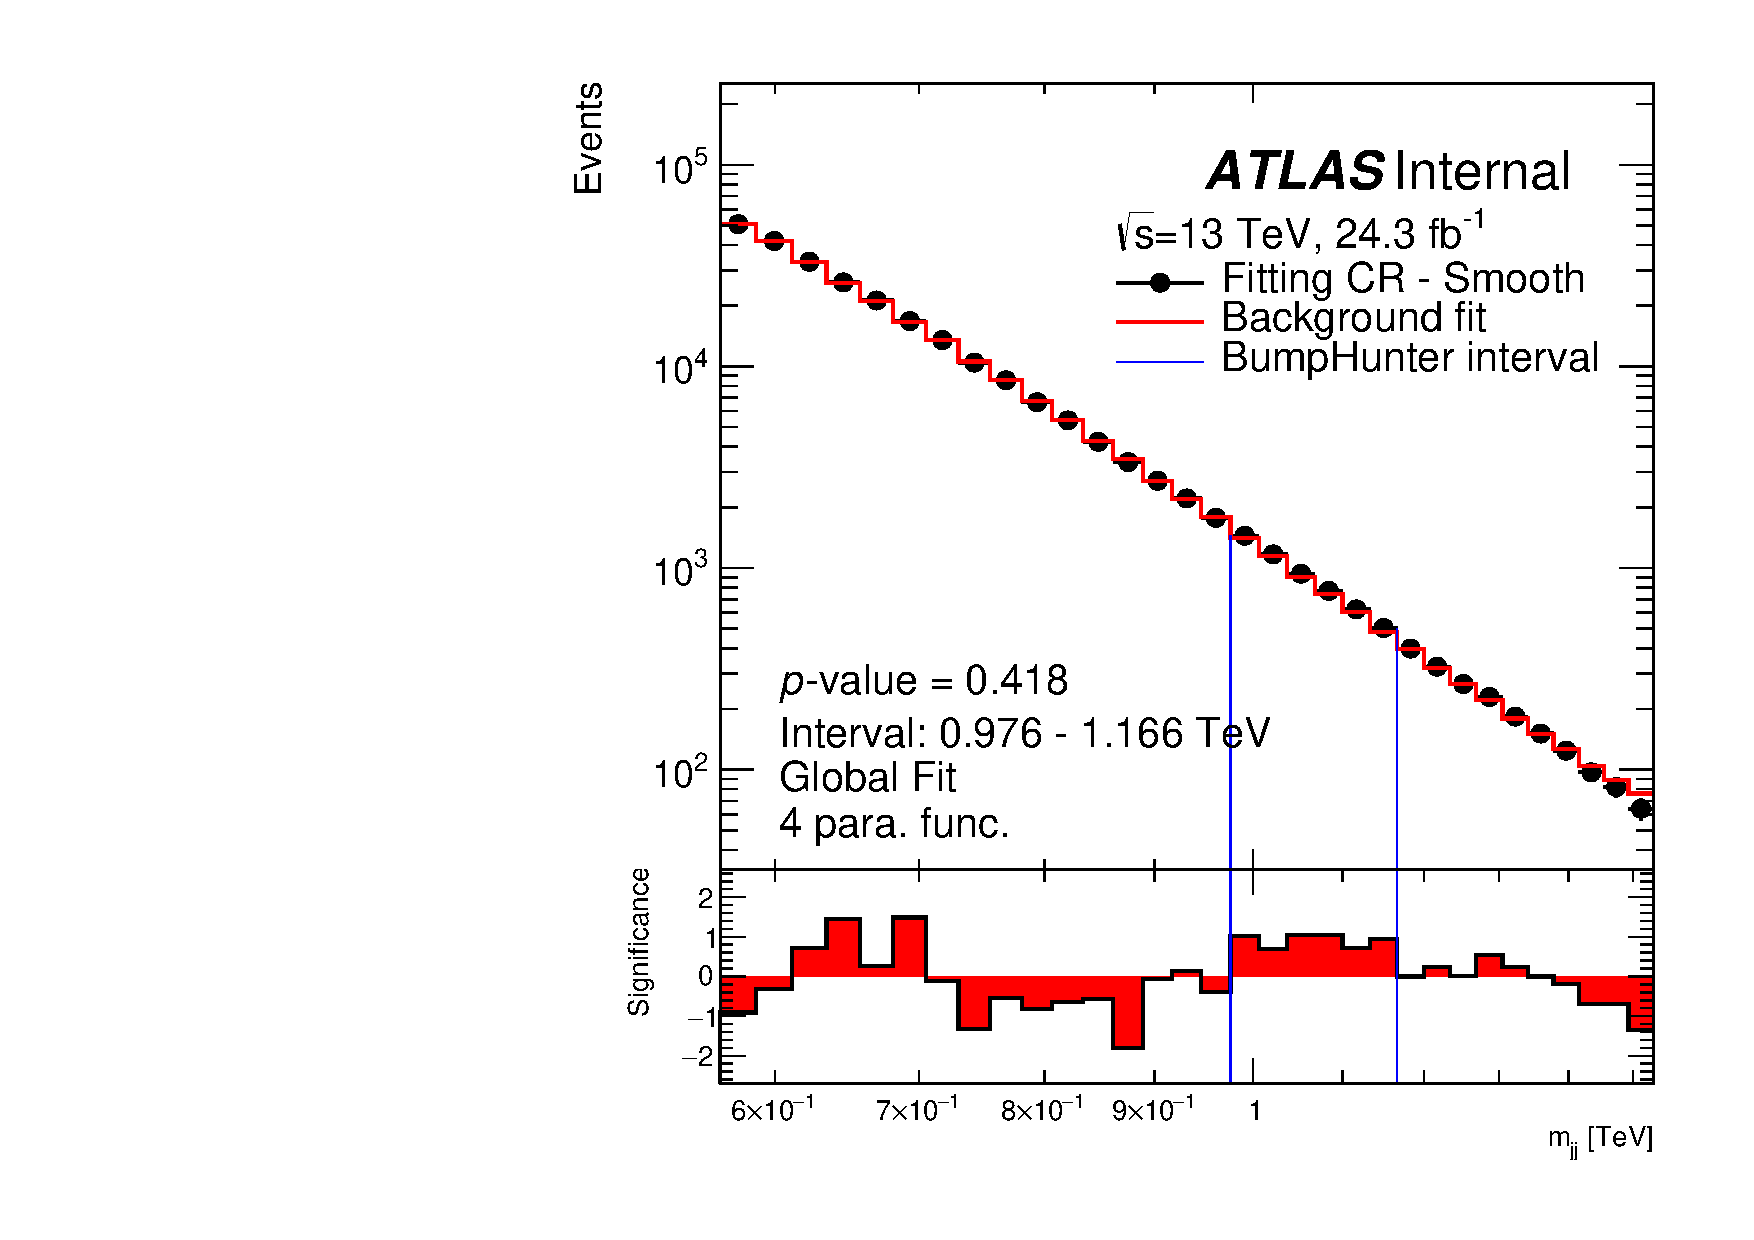
\includegraphics[width=0.45\linewidth, angle=0]{figs/Dibjet/LowMass/FitStudy_min566/globalFit_lm_bH_4para.pdf}
}
\subcaptionbox{5 parameters, Global} {
  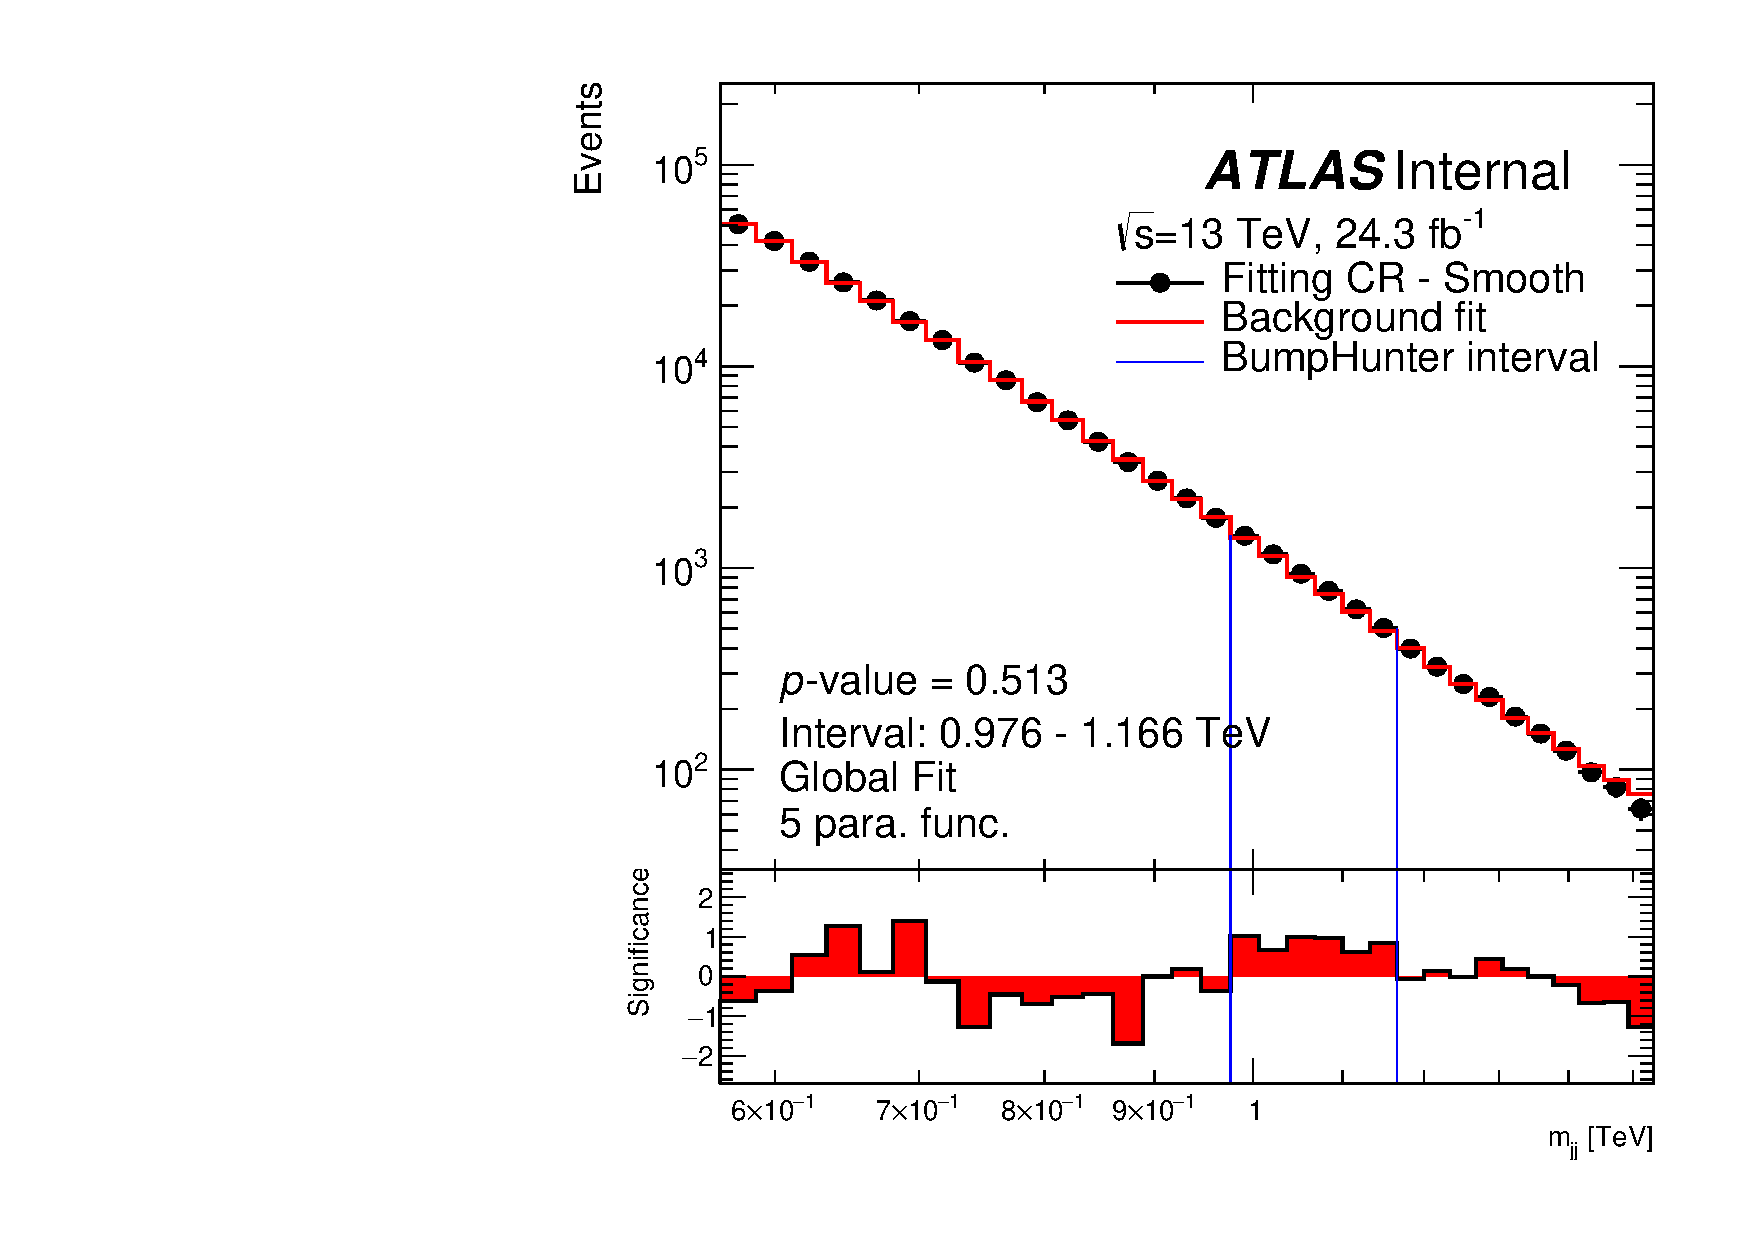
\includegraphics[width=0.45\linewidth, angle=0]{figs/Dibjet/LowMass/FitStudy_min566/globalFit_lm_bH_5para.pdf}
}

\caption{\label{fig:bhFit_lm_global}
  The global fit and \bh{} algorithm procedure run on the smooth dijet mass spectrum from the fitting control region in the low-mass category
  using the global 4 and 5 parameter dijet fit functions.
  The upper panel shows the data compared to the background estimate and the lower panel shows the significance of the difference between the two.
  The most discrepant excess as found by the \bh{} algorithm is indicated by the vertical blue lines and the \mbox{$p$-value} of this excess is printed on the plot. }
\end{figure}

%\subsubsection{High Mass}
%\label{sec:bkg-full_highmass_globalFit}

\newpage
\subsection{Sliding window background estimation (SWiFT)}\label{sec:bkg-full_swift}

In Section~\ref{sec:bkg-full_globalFit} it is shown that the global fit strategy cannot provide a
valid background estimation in the \lm{} fitting control regions.
This is not unexpected for large luminosities and wide mass ranges,
as the resulting small statistical errors and large fit ranges mean that any
differences between the underlying shape of the QCD dijet mass spectrum
and the dijet fit functions are magnified.
Therefore an alternate background modelling strategy must be used.

The Sliding Window Fit (SWiFt) background estimation breaks the spectrum up into many smaller windows,
and performs a local fit in each window to provide one point in the dijet mass background estimate.
This makes the SWiFt method more stable than the global fit at higher luminosities as the mass range of each fit is reduced.
The SWiFt background estimation procedure has been used in the inclusive dijet analysis on the full 2015+2016 ATLAS data-set~\cite{dijet-mori17_paper}.

The windows used by the SWiFT background estimate are centred at each of the
bin boundaries defined by the dijet mass bins, which are shown in Appendix~\ref{app:dijet_bins}.
The window width is defined by fixing the number of bins below the window centre ($n_{\text{Low}}$)
and fixing the number of bins above the window centre ($n_{\text{High}}$).
For this analysis symmetric windows are used, defined by their window half-width ($wHW$); i.e. $n_{\text{Low}}$ = $n_{\text{High}}$ = $wHW$.
Symmetric windows are chosen as this ensures that there will be an adequate side band on either side of the window centre where possible,
and reduces the number of parameters that have to be tested.
Windows are allowed to overlap, have no upper mass restriction and have the same lower mass bound as is used in the event-selection.
Figure~\ref{fig:bkg-lm_swiftBins} shows the SWiFt windows used in the \lm{} data-set analysis for the window half-widths of 10, 12, 14 and 16.
The procedure for choosing the window half-width is described in Section~\ref{sec:bkg-full_windowSel}

In each window a fit to the data is performed using one of the dijet fit functions listed in Table~\ref{tab:bkg-fit}.
The same function is used in all windows, with initial parameters seeded initially from a configuration file and then from the previous fit.
Each of the fits are evaluated at the dijet mass bin which is at the centre of the window, this value forms the background estimation for that bin.
A background estimation for the full dijet mass spectrum is constructed by combining the single bin background estimations from each of the window fits.

\begin{figure}[!htb]
\centering
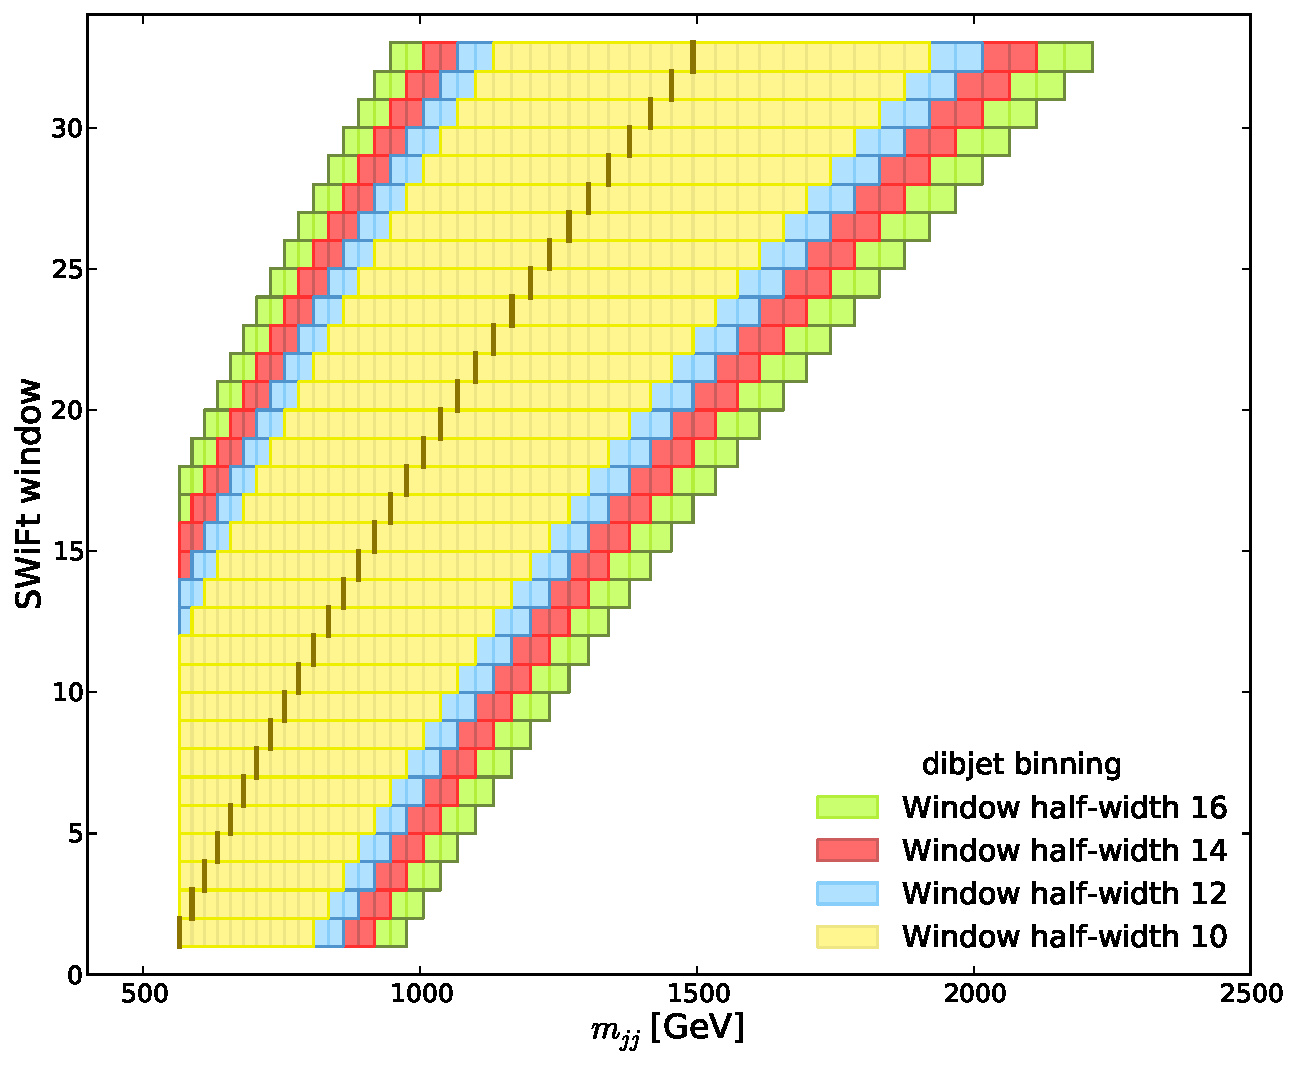
\includegraphics[width=0.6\linewidth, angle=0]{figs/Dibjet/LowMass/evt-swiftBins_min566_fl0_fh0_tr0.pdf}
\caption{\label{fig:bkg-lm_swiftBins}
  The windows used by the SWiFt background estimate in the \lm{} data-set analysis for a range of window half-widths.
  The bin centre is indicated by the black mark and the corresponding window is indicated by the coloured squares.}
\end{figure}

Once, a background estimation is constructed using the SWiFt procedure,
it is then compared to data using the \bh{} algorithm which finds the most discrepant excess region and assigns a \mbox{$p$-value} to it.
The combination of the SWiFt background estimation and \bh{} algorithm is referred to as the SWiFt search phase.
In the following SWiFt validation studies 1,000 pseudo-experiments are used to calculate the \bh{} \mbox{$p$-value}.

\subsection{SWiFT: Fit Function and Window Selection Strategy}
\label{sec:bkg-full_windowSel}

%As described above, the SWiFt background estimation involves breaking the spectrum up into smaller windows and performing a fit in each window.
%Hence, there are two key input parameters of the SWiFt background estimation:
There are two key input parameters of the SWiFt background estimation procedure:
\begin{enumerate}[leftmargin=*]
\item \textbf{The window width:}\\
  In this analysis symmetric windows are used, therefore the width of the windows is defined by the window half-width ($wHW$) parameter.\vspace{0.5em}
\item \textbf{Fit function used:}\\
  The dijet fit functions are used, as is done in the global fit strategy. \\
  The function are listed in Table~\ref{tab:bkg-fit}.
\end{enumerate}
The largest sensitivity is found by using the largest window width with the fit function with the fewest number of parameters, whilst still obtaining sufficient fit quality.
Sensitivity studies that demonstrate this statement are shown below in Section~\ref{sec:bkg-full_signalInj}.

\noindent
To define `sufficient fit quality' the following fit quality criteria used is:
\begin{itemize}[leftmargin=*]
  
\item \textbf{Global $\chi^{2}$ \mbox{$p$-value} $>$ 0.05}:\\
  The $\chi^{2}$ test statistic is calculated by comparing the data to the SWiFt background estimate.
  The global $\chi^{2}$ \mbox{$p$-value} is then calculated by comparing the test statistic
  to a $\chi^{2}$ distribution with the number of degrees of freedom equal to the number of bins
  minus the number of parameters of the fit function.\vspace{0.5em}
\item \textbf{Number of windows with Wilks' \mbox{$p$-value} $<$ 0.1 must be $\leq$ 10:}\\
  The Wilks' \mbox{$p$-value} is used to test if an additional parameter is required in the fit function
  to provide an adequate description of the data, as described in \ref{sec:bkg-wilks}. 
  However, for SWiFt it is not appropriate to require that every individual fit a Wilks' $p$-value $>$ 0.05 criteria, as done in the global fit strategy,
  as this does not account for the fact that many fits are performed and it is expected that by chance some fits would fail this requirement.
  Instead, a requirement is placed that in the large majority of windows we see no evidence that the functional form is incorrect.
\end{itemize}

To select the optimal SWiFt configuration, a predefined iterative window selection procedure is performed on the final unblinded data-set.
A predefined procedure is used as this means that the most sensitive SWiFt configuration that provides an adequate fit to the final data-set can be selected
in a manner in which no personal bias can be introduced.
%The exact procedure is tuned for the low mass and high mass searches separately so precise descriptions are found below,
%but the principle is the same for both.

%The procedure starts with the SWiFt configuration with the widest window and lowest number or parameters that will not produce spurious signal
%(see Section~\ref{sec:spuriousSignal} for the relevant spurious signal studies).
%The SWiFt background estimation is then tested against the above defined fit quality criteria.
%If the window selection fails the fit quality, then a narrower window or high-order fit function is used and again this window tested against the fit quality criteria.
%If the new window fails then again a narrower window or higher-order fit function is tested, until a window is found that passes the fit quality criteria.


%\subsubsection{Low Mass}
%\label{sec:bkg-full_lowmass_windowSel}

In the \lm{} data-set, the mass range is 566 - 1533 \GeV{}. This contains 32 bins, which in turn requires 32 windows and 32 fits.
A window half-width of 16 is  the widest window that is considered,
as this configuration is just narrower than the global fit which has been shown to give a poor fit.
A window half-width of 10 is the narrowest window considered for the purposes of the SWiFt validation tests,
as at this point the windows are becoming excessively narrow.
Figure~\ref{fig:bkg-lm_swiftBins} shows the SWiFt windows used in the for the window half-widths of 16, 14, 12 and 10

The 5 parameter dijet fit function is used for the SWiFt background estimation.
The 3 parameter fit function was not considered due to its exceptionally poor performance in the global fit, as noted in Section~\ref{sec:bkg-full_globalFit}.
The 4 parameter fit function was rejected for two reasons.
Firstly the SWiFt procedure using the 4 parameter fit function provides poor background estimates in the fit tests,
as will be demonstrated below in Section~\ref{sec:bkg-full_spuriousSignal}.
Secondly, the SWiFt background estimates for the 4 parameter fit function is less sensitive to signal than
using the SWiFt background procedure with the 5 parameter fit function and wider windows, as is demonstrated in Section~\ref{sec:bkg-full_signalInj}.

\noindent
Given the quality requirements outlined above, the strategy for selecting a window width is:
\begin{enumerate}
\item Perform the SWiFt background estimate using a window half-width of 16.
\item Use the \bh{} algorithm to search for any significant discrepant excesses (\mbox{$p$-value} $<$ 0.01),
  if one is found the SWiFt background estimate is repeated excluding the excess region.
\item Check if the fit quality tests outlined above are passed. If so select this window width.
\item If not then drop the window half-width by 2, and repeat step (2).
\end{enumerate}
This procedure is repeated until a window half-width is found where the fit quality criteria have been passed.

The step of excluding a region if the \bh{} \mbox{$p$-value} $<$ 0.01 is introduced such that
the presence of a significant signal will not bias the background estimation procedure and therefore enhance the size of observed signal.
A threshold of 0.01 is used as this signifies an excess that is greater than 2~$\sigma$ in significance,
and is consistent with the threshold used in previous dijet searches~\cite{det-thesis_kate}.
Therefore the observation of a \bh{} \mbox{$p$-value} of 0.01 becomes a critical point in this analysis,
and as such will be considered as the point at which signal becomes significant for the purposes of the following background estimation tests.
The exact procedure in the case that an excess region is excluded is outlined in Section~\ref{sec:bkg-full_signalInj}.

%\noindent
%The tests of the window selection procedure using the background-only data sets are shown in Section~\ref{sec:bkg-full_windowSelTests}

\subsubsection{High Mass} 
\label{sec:bkg-full_highmass_windowSel}

\subsection{SWiFt: Testing the window width selection procedure}
\label{sec:bkg-full_windowSelTests} 

The SWiFt window selection strategy, described in Section~\ref{sec:bkg-full_windowSel}, has been tested in the fitting test data-sets, described in Section~\ref{sec:bkg-full_stat:bkgsample}.
%The tests have been performed in both the low and high mass searches, which are described separately below.

%\subsubsection{Low Mass}
%\label{sec:bkg-full_lowmass_windowSelTests} 

Firstly, let's examine the results from the SWiFt background procedure applied to 100 different seeds of data-like spectra from the fitting control region.
Figure~\ref{fig:windowSel_dataLike} shows the cumulative probability of the two fit quality variables used in the window selection procedure,
with fraction of seeds that pass the fit quality requirements for each swift configuration printed on the bottom right of the plot.
It is shown that in $>$ 99\% of cases a window half-width in the range considered would pass the Wilks' \mbox{$p$-value} requirement
and that in $>$ 80\% of cases a window half-width in the range considered would pass the global $\chi^{2}$ \mbox{$p$-value} requirement.

\begin{figure}[!htb]
\captionsetup[subfigure]{aboveskip=0pt,justification=centering}
\centering
\subcaptionbox{Global $\chi^{2}$ \mbox{$p$-value},\\ 5 parameter function} {
  \includegraphics[width=0.49\linewidth, angle=0,page=7]{figs/Dibjet/LowMass/FitStudy_min566/windowSel_corrFitCR_dataLike_5para.pdf}
}  \hspace{-8mm}
\subcaptionbox{Number of window fits with\\Wilks' \mbox{$p$-value} $<$ 0.1,\\ 5 parameter function} {
  \includegraphics[width=0.49\linewidth, angle=0,page=9]{figs/Dibjet/LowMass/FitStudy_min566/windowSel_corrFitCR_dataLike_5para.pdf}
}

\caption{\label{fig:windowSel_dataLike}
  The cumulative probability of the global $\chi^{2}$ \mbox{$p$-value}, %global Kolmogorov-Smirnov \mbox{$p$-value}
  and number of window fits with Wilks' \mbox{$p$-value} $<$ 0.1 of the SWiFt background estimation for
  100 data-like distributions taken from the fitting control region in the low mass region.
  The SWiFt procedure has been performed using the 5 parameter dijet fit function
  for the range of window half-widths ($wHW$) of 10 to 16.
  The fraction of seeds that pass the fit quality requirements for each swift configuration is shown in the bottom right of the plot.
}
\end{figure}

The window selection procedure is also tested using the 3 \ifb{} subset of data.
Figure~\ref{fig:windowSel_subset} shows the fit quality measures used in the window width selection procedure,
using a range of window half-widths of 16 to 10, for both the 4 and 5 parameter fit function.
The requirements placed on each fit quality measure by the window selection procedure are indicated by dotted lines on the figure.
According to the window selection procedure the 5 parameter fit function with a window half-width of 16 would have been selected,
although the 4 parameter fit function with window half-width of 16 has also passed the fit quality criteria.

\begin{figure}[!htb]
\captionsetup[subfigure]{aboveskip=0pt,justification=centering}
\centering
\subcaptionbox{Global $\chi^{2}$ \mbox{$p$-value}} {
  \includegraphics[width=0.45\linewidth, angle=0,page=2]{figs/Dibjet/LowMass/FitStudy_min566/windowSel_subset.pdf}
}\hspace{-8mm}
%\subcaptionbox{Global Kolmogorov Smirnov \mbox{$p$-value}} {
%  \includegraphics[width=0.49\linewidth, angle=0,page=1]{figs/Dibjet/LowMass/FitStudy_min566/windowSel_subset.pdf}
%} \\
\subcaptionbox{Number of window fits with\\ Wilks' \mbox{$p$-value} $<$ 0.1} {
  \includegraphics[width=0.45\linewidth, angle=0,page=4]{figs/Dibjet/LowMass/FitStudy_min566/windowSel_subset.pdf}
}

\caption{\label{fig:windowSel_subset}
  An illustration of the window selection procedure for a 3 \ifb{} subset of \lm{} data.
  It shows the global $\chi^{2}$ \mbox{$p$-value}, %global Kolmogorov-Smirnov \mbox{$p$-value}
  and number of window fits with Wilks' \mbox{$p$-value} $<$ 0.1 for the SWiFt background estimate
  using a range of window half-widths ($wHW$) and number of parameters (nPars) of the dijet fit function.
  The dotted lines indicate thresholds that are used in the window selection procedure.
}
\end{figure}

To illustrate the background estimations being used in the above window selection procedure,
Figure~\ref{fig:bhFit_lm_subset} shows the SWiFt search phase performed on the dijet mass spectrum of the 3 \ifb{} data subset,
for the 4 and 5 parameter fit function for a window half-width of 16, which both pass the fit quality criteria.
The blue-lines indicate the largest excess found by the \bh{} algorithm and the \mbox{$p$-value} assigned is printed on the plot. 
In both cases the background is well modelled and, as expected, there is no significant excess found.

\begin{figure}[!htb]
\captionsetup[subfigure]{aboveskip=0pt,justification=centering}
\centering
\subcaptionbox{4 parameter function,\\ $wHW$ = 16} {
  \includegraphics[width=0.45\linewidth, angle=0]{figs/Dibjet/LowMass/FitStudy_min566/bhFit_subset_4para_low16_high16.pdf}
}
\subcaptionbox{5 parameter function,\\ $wHW$ = 16} {
  \includegraphics[width=0.45\linewidth, angle=0]{figs/Dibjet/LowMass/FitStudy_min566/bhFit_subset_5para_low16_high16.pdf}
}

\caption{\label{fig:bhFit_lm_subset}
  The SWiFt search phase run on a 3 \ifb{} subset of the \lm{} data-set.
  The SWiFt procedure has been run for the 4 and 5 parameter fit function for a window half-width ($wHW$) of 16.
  The upper panel shows the data compared to the background estimate and the lower panel shows the significance of the difference between the two.
  The most discrepant excess as found by the \bh{} algorithm is indicated by the vertical blue lines and the \mbox{$p$-value} of this excess is printed on the plot. }
\end{figure}

It is notable that the window selection procedure in the subset of data has chosen a wide window and
could have chosen the lower order function, in contrast to the fitting control region case. 
This shows that either the fitting control region often selects narrower windows
because it is not a perfect representation of the true dijet mass spectra
or because at the higher precision of the 24.3 \ifb{} narrower windows are required than at 3 \ifb{}.
Either way, this shows the utility of choosing the window width on the final data-set using a pre-defined procedure.

%\subsubsection{High Mass}
%\label{sec:bkg-full_highmass_windowSelTests} 

\newpage
\subsection{SWiFt: Spurious Signal Tests}
\label{sec:bkg-full_spuriousSignal}

As described in Section~\ref{sec:bkg-summer_spusig}, it is important to demonstrate that the background estimation strategy
provides a valid representation of the true background spectrum meaning that fit biases and spurious signal cannot occur.
To show this, the SWiFt search phase is performed to many background-only representative
data-sets and the global distribution of the \bh{} \mbox{$p$-values} is studied.
Only windows widths that show no evidence of spurious signal are considered by window selection procedure.

For the spurious signal tests the SWiFt search phase is performed with the 4 and 5 parameter fit function
for a symmetric window with window half-width range of 10 to 16, giving 8 different window width and fit function combinations.

Firstly, the SWiFt procedure is tested using the smooth dijet mass spectrum from the fitting control region
where the errors are set to be Poisson like,
as described in Section~\ref{sec:bkg-full_bkgsample}.
Performing the SWiFt search phase to the smooth dijet mass spectra gives a direct comparison
of any fit biases relative to the background fluctuations expected in data.
Figure~\ref{fig:bhFit_lm_corrFitCR_smooth} shows the SWiFt search phase
performed on the smooth dijet mass spectrum taken from the fitting control region,
for a SWiFt configuration using the 4 and 5 parameter dijet fit functions and a $wHW$ of 16 and 10,
the full set of plots for all SWiFt configurations considered can be found in Appendix~\ref{app:lowMass_Swift}.
The blue-lines indicate the largest excess found by the \bh{} algorithm and the \mbox{$p$-value} assigned is printed on the plot. 

\begin{figure}[!htb]
\captionsetup[subfigure]{aboveskip=0pt,justification=centering}
\centering
\subcaptionbox{4 parameter function,\\ $wHW$ = 16} {
  \includegraphics[width=0.45\linewidth, angle=0]{figs/Dibjet/LowMass/FitStudy_min566/bhFit_corrFitCR_smooth_4para_low16_high16.pdf}
}
%\subcaptionbox{4 parameter fit, $wHW$ = 14} {
%  \includegraphics[width=0.45\linewidth, angle=0]{figs/Dibjet/LowMass/FitStudy_min566/bhFit_corrFitCR_smooth_4para_low14_high14.pdf}
%}
%\subcaptionbox{4 parameter fit, $wHW$ = 12} {
%  \includegraphics[width=0.45\linewidth, angle=0]{figs/Dibjet/LowMass/FitStudy_min566/bhFit_corrFitCR_smooth_4para_low12_high12.pdf}
%}
\subcaptionbox{4 parameter function,\\ $wHW$ = 10} {
  \includegraphics[width=0.45\linewidth, angle=0]{figs/Dibjet/LowMass/FitStudy_min566/bhFit_corrFitCR_smooth_4para_low10_high10.pdf}
}
\subcaptionbox{5 parameter function,\\ $wHW$ = 16} {
  \includegraphics[width=0.45\linewidth, angle=0]{figs/Dibjet/LowMass/FitStudy_min566/bhFit_corrFitCR_smooth_5para_low16_high16.pdf}
}
%\subcaptionbox{5 parameter function,\\ $wHW$ = 14} {
%  \includegraphics[width=0.45\linewidth, angle=0]{figs/Dibjet/LowMass/FitStudy_min566/bhFit_corrFitCR_smooth_5para_low14_high14.pdf}
%}
%\subcaptionbox{5 parameter fit, $wHW$ = 12} {
%  \includegraphics[width=0.45\linewidth, angle=0]{figs/Dibjet/LowMass/FitStudy_min566/bhFit_corrFitCR_smooth_5para_low12_high12.pdf}
%}
\subcaptionbox{5 parameter function,\\ $wHW$ = 10} {
  \includegraphics[width=0.45\linewidth, angle=0]{figs/Dibjet/LowMass/FitStudy_min566/bhFit_corrFitCR_smooth_5para_low10_high10.pdf}
}

\caption{\label{fig:bhFit_lm_corrFitCR_smooth}
  The SWiFt search phase run on the smooth distribution from the fitting control region in the low-mass category.
  The SWiFt procedure has been run for the 4 and 5 parameter fit function for a window half-width ($wHW$) 10 and 16.
  The upper panel shows the data compared to the background estimate and the lower panel shows the significance of the difference between the two.
  The most discrepant excess as found by the \bh{} algorithm is indicated by the vertical blue lines and the \mbox{$p$-value} of this excess is printed on the plot. }
\end{figure}

As was discussed in Section~\ref{sec:bkg-full_globalFit}, in the case of the smooth spectrum the \bh{} \mbox{$p$-value} provides an approximate estimation
of the size of the largest fit bias relative to the size of the largest excesses expected in data due to statistical fluctuations.
If the fit bias is larger than the statistical fluctuations then this is an indication that spurious signal can occur. 
For the 4 parameter dijet fit function with a window half-width of 16 a \bh{} $p$-value of 0.298 is observed indicating that
there is a fit bias which is large relative to the expected statistical fluctuations.
It is also notable that for the 4 parameter dijet fit function there is a large deficit observed in the middle of the mass range for both window half-widths shown.
In the 5 parameter fit function \bh{} $p$-values of 0.826 and 0.987 are observed in the window half-width of 16 and 10 respectively,
which indicates that the largest fit bias is not larger than the size of the excesses expected in data.

The SWiFt search phase performed on the smooth distribution provides a good visual representation and approximate size of possible fit biases,
but a more robust approach is to determine if spurious signal can occur in the final data-set where Poisson fluctuations are present.
To do this the SWiFt search phase is applied to many data-like dijet mass spectra,
where Poisson fluctuations are applied to the fitting control region as described in Section~\ref{sec:bkg-full_bkgsample}.
Figure~\ref{fig:bhFit_lm_corrFitCR_dataLike} shows an example of the SWiFt search phase performed on a data-like dijet mass spectrum taken from the fitting control region.
%Again, all 8 window width and fit function choice combinations studied are considered
The SWiFt configurations with a window half-width of 16 for the 4 and 5 parameter dijet fit function are shown, the full set can be found in Appendix~\ref{app:lowMass_Swift}.
Again, the largest excess found by the \bh{} algorithm and the \mbox{$p$-value} assigned is indicated on the plot.
It is observed that the fit biases noted in Figure~\ref{fig:bhFit_lm_corrFitCR_smooth} are still visible in the 4 parameter case.
In the 5 parameter case the \bh{} algorithm has not identified a discrepant excess indicating
there is no spurious signal for this particular data-like spectrum.

\begin{figure}[!htb]
\captionsetup[subfigure]{aboveskip=0pt,justification=centering}
\centering
\subcaptionbox{4 parameter function,\\ $wHW$ = 16} {
  \includegraphics[width=0.45\linewidth, angle=0]{figs/Dibjet/LowMass/FitStudy_min566/bhFit_corrFitCR_dataLike_v13_4para_low16_high16.pdf}
}
%\subcaptionbox{4 parameter function,\\ $wHW$ = 14} {
%  \includegraphics[width=0.45\linewidth, angle=0]{figs/Dibjet/LowMass/FitStudy_min566/bhFit_corrFitCR_dataLike_v13_4para_low14_high14.pdf}
%}
%\subcaptionbox{4 parameter function,\\ $wHW$ = 12} {
%  \includegraphics[width=0.45\linewidth, angle=0]{figs/Dibjet/LowMass/FitStudy_min566/bhFit_corrFitCR_dataLike_v13_4para_low12_high12.pdf}
%}
%\subcaptionbox{4 parameter function,\\ $wHW$ = 10} {
%  \includegraphics[width=0.45\linewidth, angle=0]{figs/Dibjet/LowMass/FitStudy_min566/bhFit_corrFitCR_dataLike_v13_4para_low10_high10.pdf}
%}
\subcaptionbox{5 parameter function,\\ $wHW$ = 16} {
  \includegraphics[width=0.45\linewidth, angle=0]{figs/Dibjet/LowMass/FitStudy_min566/bhFit_corrFitCR_dataLike_v13_5para_low16_high16.pdf}
}
%\subcaptionbox{5 parameter function,\\ $wHW$ = 14} {
%  \includegraphics[width=0.45\linewidth, angle=0]{figs/Dibjet/LowMass/FitStudy_min566/bhFit_corrFitCR_dataLike_v13_5para_low14_high14.pdf}
%}
%\subcaptionbox{5 parameter function,\\ $wHW$ = 12} {
%  \includegraphics[width=0.45\linewidth, angle=0]{figs/Dibjet/LowMass/FitStudy_min566/bhFit_corrFitCR_dataLike_v13_5para_low12_high12.pdf}
%}
%\subcaptionbox{5 parameter function,\\ $wHW$ = 10} {
%  \includegraphics[width=0.45\linewidth, angle=0]{figs/Dibjet/LowMass/FitStudy_min566/bhFit_corrFitCR_dataLike_v13_5para_low10_high10.pdf}
%}

\caption{\label{fig:bhFit_lm_corrFitCR_dataLike}
  The SWiFt search phase run on a data-like dijet mass spectrum of the the fitting control region in the low-mass category.
  %The SWiFt procedure has been run for the 4 and 5 parameter fit function for a window half-width ($wHW$) range of 10 to 16.
  The SWiFt procedure has been run for the 4 and 5 parameter fit function for a window half-width ($wHW$) of 16.
  The upper panel shows the data compared to the background estimate and the lower panel shows the significance of the difference between the two.
  The most discrepant excess as found by the \bh{} algorithm is indicated by the vertical blue lines and the \mbox{$p$-value} of this excess is printed on the plot. 
}
\end{figure}

To provide a quantitative statement on if spurious signal is observed,
this process is repeated for 100 data-like dijet mass spectra and the distribution of \bh{} \mbox{$p$-value}s is studied to search for evidence of spurious signal.
500 data-like distributions are used in the case of the 5 parameter fit for window half-widths of 14 and 16
as extra precision is required to make the necessary conclusion for these configurations.
Each data-like distribution is referred to as a `seed', which denotes the seed used in the random Poisson fluctuation generator.
%In the case of the 5 parameter fit function with a window half-width of 16, which is the widest window that will be used in data and hence the most
%challenging fit that will be performed, this procedure was performed with 450 different data-like distributions to increase statistical precision.
Figure~\ref{fig:bumpH_spuriousSignal} shows the normalised distribution of \mbox{$p$-value}s for the ensemble of data-like distributions
for a subset of the SWiFt configurations considered, the full range of plots can be found in Appendix~\ref{app:lowMass_Swift}.
%for the 8 combinations of window/function choice considered.

\begin{figure}[!htb]
\captionsetup[subfigure]{aboveskip=0pt,justification=centering}
\centering
\subcaptionbox{4 parameter function,\\ $wHW$ = 16} {
  \includegraphics[width=0.45\linewidth, angle=0]{figs/Dibjet/LowMass/FitStudy_min566/pVal_bumpHunter_corrFitCR_4para_low16_high16.pdf}
}                                                                                              
%\subcaptionbox{4 parameter function,\\ $wHW$ = 14} {                                                    
%  \includegraphics[width=0.45\linewidth, angle=0]{figs/Dibjet/LowMass/FitStudy_min566/pVal_bumpHunter_corrFitCR_4para_low14_high14.pdf}
%}                                                                                              
%\subcaptionbox{4 parameter function,\\ $wHW$ = 12} {                                                    
%  \includegraphics[width=0.45\linewidth, angle=0]{figs/Dibjet/LowMass/FitStudy_min566/pVal_bumpHunter_corrFitCR_4para_low12_high12.pdf}
%}                                                                                              
\subcaptionbox{4 parameter function,\\ $wHW$ = 10} {                                                    
  \includegraphics[width=0.45\linewidth, angle=0]{figs/Dibjet/LowMass/FitStudy_min566/pVal_bumpHunter_corrFitCR_4para_low10_high10.pdf}
}                                                                                              
\subcaptionbox{5 parameter function,\\ $wHW$ = 16} {                                                    
  \includegraphics[width=0.45\linewidth, angle=0]{figs/Dibjet/LowMass/FitStudy_min566/pVal_bumpHunter_corrFitCR_5para_low16_high16.pdf}
}                                                                                              
\subcaptionbox{5 parameter function,\\ $wHW$ = 14} {                                                    
  \includegraphics[width=0.45\linewidth, angle=0]{figs/Dibjet/LowMass/FitStudy_min566/pVal_bumpHunter_corrFitCR_5para_low14_high14.pdf}
}                                                                                              
%\subcaptionbox{5 parameter function,\\ $wHW$ = 12} {                                                    
%  \includegraphics[width=0.45\linewidth, angle=0]{figs/Dibjet/LowMass/FitStudy_min566/pVal_bumpHunter_corrFitCR_5para_low12_high12.pdf}
%}                                                                                              
%\subcaptionbox{5 parameter function,\\ $wHW$ = 10} {                                                    
%  \includegraphics[width=0.45\linewidth, angle=0]{figs/Dibjet/LowMass/FitStudy_min566/pVal_bumpHunter_corrFitCR_5para_low10_high10.pdf}
%}

\caption{\label{fig:bumpH_spuriousSignal}
  This figure shows the normalised distribution of \bh{} \mbox{$p$-value}s from performing the SWiFt background estimate to an ensemble of
  data-like distributions taken from the fitting control region in the low-mass category.
  This is repeated for the 4 and 5 parameter fit function for a symmetric window with window half-width ($wHW$) range of 10 to 16,
  giving the 8 different window width and fit function combinations.
  The number of data-like distributions or seeds is given on the plot.
}
\end{figure}

Furthermore, Table~\ref{tab:bumpH_lm_spuriousSignal} shows the percentage of data-like distributions (or seeds)
that have a \bh{} \mbox{$p$-value} less than %0.1,
0.05 and 0.01 for the full range of SWiFt configurations considered;
in particular 0.01 is important as it is the threshold for an excess region to be considered significant enough
to exclude from the background estimate procedure.

\begin{table}[!ht]
\centering
\begin{tabular}{|c|c||c|c|c|c|}
  \hline
\multirow{2}{*}{nPars} & \multirow{2}{*}{$wHW$} &\multicolumn{2}{c|}{Fraction of Seeds with BH \mbox{$p$-value} \textless} &  \multirow{2}{*}{nSeeds} \\ \cline{3-4} 
                       &                     & 0.05                & 0.01            &        \\ 
  \hline
  4 &   16 &  31\%   (26-35\%)   &  7.0\% (4-10\%)  & 100  \\
  4 &   14 &  13\%   (9-16\%)    &  4.0\% (2-6\%)   & 100  \\
  4 &   12 &  10\%   (7-13\%)    &  4.0\% (2-6\%)   & 100  \\
  4 &   10 &  2\%   (1-4\%)      &  1.0\% (0-3\%)   & 100  \\
  \hline
  5 &   16 &  4.0\% (3.2-4.9\%)  &  1.2\% (0.8-1.8) & 500  \\
  5 &   14 &  2.4\% (1.8-3.1\%)  &  0.8\% (0.5-1.3) & 500  \\
  5 &   12 &  1\%   (0-3\%)      &  0.0\%  (0-1\%)  & 100  \\
  5 &   10 &  2\%   (1-4\%)      &  1.0\%  (0-3\%)  & 100  \\
  \hline
\end{tabular}

\caption{\label{tab:bumpH_lm_spuriousSignal}
  A summary of the fraction of data-like distributions 
  with a \bh{} \mbox{$p$-value} less than certain threshold values,
  when the SWiFt search phase with the 4 and 5 parameter fit function
  and various window half-widths ($wHW$) is performed to an ensemble of data-like distributions
  taken from the fitting control region in the low-mass category.
  The numbers in brackets represent a 1$\sigma$ confidence interval on the fraction.}
\end{table}


It is observed that for the 4 parameter fit function and a window half-width of 10, 12 and 14 there is a clear bias towards
low \bh{} \mbox{$p$-value}s.
In particular, it is notable that significantly more than 1\% of seeds have \bh{} \mbox{$p$-value} of less than 0.01.
Hence, it is concluded that all SWiFt configurations with the 4 parameter fit function with window half-width greater than 10
show evidence of spurious signal.
For the 4 parameter fit function with a window half-width of 10, there is no evidence of spurious signal,
However this configuration is not used as it it is less sensitivity to signal than the 5 parameter fit with wider windows, as shown will be shown in Section~\ref{sec:bkg-full_signalInj}.
In the case of the 5 parameter fit function there is no significant bias towards low \bh{} \mbox{$p$-value}s,
specifically the number of seeds with a \bh{} \mbox{$p$-value} of less than 0.01 is consistent with expectations.
There is a deficit of seeds with a \bh{} $p$-value $>$ 0.9 for all configurations which is due to the fact that the
dijet mass spectrum itself of the fitting control region is not perfectly smooth.

Therefore, it is concluded that for the 5 parameter dijet fit function there is no evidence that spurious signal can occur in the window half-widths considered.

%\begin{table}[!ht]
%\centering
%\begin{tabular}{|c|c||c|c|c|c|}
%  \hline
%\multirow{2}{*}{nPars} & \multirow{2}{*}{$wHW$} &\multicolumn{3}{c|}{Fraction of Seeds with BH \mbox{$p$-value} \textless} & nSeeds \\ \cline{3-5} 
%                       &                      &    0.1                  & 0.05                & 0.01            &        \\ 
%  \hline
%  4 &   16& 66.0\% (61.20-70.59) & 39.0\% (34.24-43.91) & 16.0\% (12.58-19.87) &  100  \\
%  4 &   14& 32.0\% (27.49-36.74) & 19.0\% (15.31-23.10) &  8.0\% (5.56-11.00) &  100  \\
%  4 &   12& 20.0\% (16.22-24.17) & 12.0\% (9.01-15.49) &  6.0\% (3.91-8.68) &  100  \\
%  4 &   10& 11.0\% (8.14-14.38) &  4.0\% (2.32-6.30) &  2.0\% (0.88-3.80) &  100  \\
%  \hline
%  5 &   16& 18.1\% (16.44-19.94) &  6.0\% (4.96-7.12) &  0.8\% (0.47-1.32) &  485  \\
%  5 &   14&  5.2\% (4.26-6.26)   &  2.6\% (1.95-3.38) &  0.6\% (0.31-1.03) &  500  \\
%  5 &   12&  3.6\% (2.83-4.50)   &  1.8\% (1.26-2.47) &  0.4\% (0.17-0.77) &  500  \\
%  5 &   10&  7.4\% (5.14-10.20)  &  2.8\% (1.46-4.70) &  0.9\% (0.25-2.29) &  108  \\
%  \hline
%\end{tabular}
%
%\caption{\label{tab:bumpH_lm_spuriousSignal}
%  A summary of the fraction of data-like distributions 
%  with a \bh{} \mbox{$p$-value} less than certain threshold values,
%  when the SWiFt search phase with the 4 and 5 parameter fit function
%  and various window half-widths ($wHW$) is performed to an ensemble of data-like distributions
%  taken from the fitting control region in the low-mass category.
%  The numbers in brackets represent a 1$\sigma$ confidence interval on the fraction.}
%\end{table}

\FloatBarrier

\subsection{SWiFt: Signal Injection Tests}
\label{sec:bkg-full_signalInj}

In the previous two subsections it is shown that the SWiFt background estimate procedure is effective in the case that there is no signal.
However, it is also required to test the SWiFt procedure in the case that signal is present, to show that signal can be identified and the remaining background estimate is valid.
This test is performed by injecting the signal dijet mass templates, described in Section~\ref{sec:evt-s+b}, into the background-only test data-sets and performing the SWiFt search phase.
The size of the signal is varied by applying a normalisation factor to the simulated signal templates,
and as such the size of signal in these studies will be labelled relative to this nominal cross-section (i.e. xs*2 = normalisation factor of 2).

To identify signal, the SWiFt search phase uses the \bh{} algorithm to identify the most discrepant excess region and assigns that region a \mbox{$p$-value}.
If the \mbox{$p$-value} is $<$ 0.01 then a exclusion region procedure is used to reduce any bias from a large signal in the background estimation.
The exclusion region procedure is as follows.
\begin{enumerate}[leftmargin=*]
\item If a discrepant excess is found, define an exclusion region as the excess
  region identified by the \bh{} algorithm with an additional \mjj{} bin added to the low mass side.
  The additional bin has been shown to help reduce any bias from signal~\cite{dijet-mori16_paper}.
\item Re-run SWiFt, ignoring the exclusion region in all fits and fit quality measures.
\item A new excess is found using the new background and the \bh{} algorithm,
  the excess can include bins in the exclusion region.
\item If the new excess is not covered by the exclusion region, then the signal was not contained within the exclusion region.
  Thus, the excess region is then widened and the procedure returns to Step 2.
\item Otherwise, the new background is tested against the fit quality criteria outlined in~\ref{sec:bkg-full_windowSel}.
\item If the fit quality criteria is failed, then a narrower window is tested.
\item If the fit quality criteria is passed, the background estimation is used.
\end{enumerate}
This process will be illustrated with an example below for clarity.
 
\noindent
In the following section we will describe two signal injection tests:
\begin{enumerate}
  \item\textbf{Sensitivity Studies}\\
  This test is to show that the procedure is sensitive to signal,
  and to show which choices of window half-width and fit function are most sensitive.
  This is performed by studying the \bh{} \mbox{$p$-value}s for various SWiFt configurations for the signal injected spectra described above.
  A \mbox{$p$-value} $<$ 0.01 will be counted as a success, as this is a critical point  where the region exclusion criteria is triggered.
  For comparing the sensitivity of two SWiFt configurations a comparison of
  \bh{} \mbox{$p$-value}s is used, where a lower \mbox{$p$-value} indicates a higher sensitivity.\vspace{1em}
  
  \item\textbf{Robustness of Window Selection Procedure}\\
  This test is to show that in the presence of signal, the window selection procedure is able to select a window.
  To perform this a fit from the sensitivity study that passed the \bh{} \mbox{$p$-value} $<$ 0.01 test is taken,
  and the region exclusion and  window selection procedure described in the previous paragraph is applied.
\end{enumerate}

%\noindent
%Again, the low mass and high mass sections of the analysis are described separately for clarity.

%\subsubsection{Low Mass}
%\label{sec:bkg-full_lowmass_signalInj}

For these tests a Monte Carlo simulated dijet mass signal template of a sequential standard model (SSM) $Z'$ boson with a simulated mass of 600, 800 and 1000 GeV
has been injected into a data-like dijet mass spectrum taken from the background-only fitting control region.
The cross-section of the template uses the nominal Monte-Carlo simulated cross-section from { \sc Pythia8} multiplied by a factor of 1, 2 or 3.

As an example let's first consider the $Z'$ boson with mass of 800 GeV.
The  SWiFt search phase is performed on a data-like mass spectrum
with an injected  $Z'$ boson with mass of 800 GeV and the nominal cross section.
Figure~\ref{fig:bhFit_lm_corrFitCR_dataLike_inj_Zprimebb800_xsFactor1}
shows the results of the SWiFt search phase
using the 5 parameter fit function and a range of window half-widths of 16 to 10.
For all window widths, the \bh{} algorithm has correctly identified the signal region location
and in the case of the window half-width of 14 and 16, has assigned a significant \mbox{\mbox{$p$-value}} ($<$ 0.01).

\begin{figure}[!htb]
\captionsetup[subfigure]{aboveskip=0pt,justification=centering}
\centering
%\subcaptionbox{4 parameter function,\\ $wHW$ = 16} {
%  \includegraphics[width=0.45\linewidth, angle=0]{figs/Dibjet/LowMass/FitStudy_min566/bhFit_corrFitCR_dataLike_4para_low16_high16_inj_Zprimebb800_xsFactor1.pdf}
%}
%\subcaptionbox{4 parameter function,\\ $wHW$ = 14} {
%  \includegraphics[width=0.45\linewidth, angle=0]{figs/Dibjet/LowMass/FitStudy_min566/bhFit_corrFitCR_dataLike_4para_low14_high14_inj_Zprimebb800_xsFactor1.pdf}
%}\\
%\subcaptionbox{4 parameter function,\\ $wHW$ = 12} {
%  \includegraphics[width=0.45\linewidth, angle=0]{figs/Dibjet/LowMass/FitStudy_min566/bhFit_corrFitCR_dataLike_4para_low12_high12_inj_Zprimebb800_xsFactor1.pdf}
%}
%\subcaptionbox{4 parameter function,\\ $wHW$ = 10} {
%  \includegraphics[width=0.45\linewidth, angle=0]{figs/Dibjet/LowMass/FitStudy_min566/bhFit_corrFitCR_dataLike_4para_low10_high10_inj_Zprimebb800_xsFactor1.pdf}
%}
\subcaptionbox{5 parameter function,\\ $wHW$ = 16} {
  \includegraphics[width=0.45\linewidth, angle=0]{figs/Dibjet/LowMass/FitStudy_min566/bhFit_corrFitCR_dataLike_5para_low16_high16_inj_Zprimebb800_xsFactor1.pdf}
}
\subcaptionbox{5 parameter function,\\ $wHW$ = 14} {
  \includegraphics[width=0.45\linewidth, angle=0]{figs/Dibjet/LowMass/FitStudy_min566/bhFit_corrFitCR_dataLike_5para_low14_high14_inj_Zprimebb800_xsFactor1.pdf}
}\\
\subcaptionbox{5 parameter function,\\ $wHW$ = 12} {
  \includegraphics[width=0.45\linewidth, angle=0]{figs/Dibjet/LowMass/FitStudy_min566/bhFit_corrFitCR_dataLike_5para_low12_high12_inj_Zprimebb800_xsFactor1.pdf}
}
\subcaptionbox{5 parameter function,\\ $wHW$ = 10} {
  \includegraphics[width=0.45\linewidth, angle=0]{figs/Dibjet/LowMass/FitStudy_min566/bhFit_corrFitCR_dataLike_5para_low10_high10_inj_Zprimebb800_xsFactor1.pdf}
}

\caption{\label{fig:bhFit_lm_corrFitCR_dataLike_inj_Zprimebb800_xsFactor1}
  The SWiFt search phase run on a data-like distribution
  from the fitting control region with a simulated SSM $Z'$ boson of mass 800 GeV injected.
  The SWiFt procedure has been run for the 5 parameter fit function for a window half-width ($wHW$) range of 10 to 16.
}
\end{figure}

Therefore, in in the case of the window half-width of 14 and 16 the region exclusion procedure is applied.
The region excluded is 705-834~GeV, derived by adding one bin on the low mass side of the excess region identified by the \bh{} algorithm (730-834~GeV).
Figure~\ref{fig:bhFit_lm_corrFitCR_dataLike_inj_Zprimebb800_xsFactor1_removedWindow} shows the SWiFt search phase
performed on the same spectrum when a region exclusion of 705-834 GeV is applied.
The new excess found lies within the exclusion region which indicates that any fit bias from the signal has been successfully removed
and therefore the exclusion region does not need to be widened.

\begin{figure}[!htb]
\captionsetup[subfigure]{aboveskip=0pt,justification=centering}
\centering
\subcaptionbox{Exclusion Region 705-807 GeV,\\ $wHW$ = 16} {
  \includegraphics[width=0.45\linewidth, angle=0]{figs/Dibjet/LowMass/FitStudy_min566/bhFit_corrFitCR_dataLike_5para_low16_high16_inj_Zprimebb800_xsFactor1_removedWindow.pdf}
}
\subcaptionbox{Exclusion Region 705-834 GeV,\\ $wHW$ = 14} {
  \includegraphics[width=0.45\linewidth, angle=0]{figs/Dibjet/LowMass/FitStudy_min566/bhFit_corrFitCR_dataLike_5para_low14_high14_inj_Zprimebb800_xsFactor1_removedWindow.pdf}
}

\caption{\label{fig:bhFit_lm_corrFitCR_dataLike_inj_Zprimebb800_xsFactor1_removedWindow}
  The SWiFt search phase run on a data-like distribution
  from the fitting control region with a simulated SSM $Z'$ boson of mass 800 GeV and the nominal cross-section injected.
  The SWiFt search phase is run for the 5 parameter fit function for a window half-width ($wHW$) of (a) 16 and (b) 14
  with an exclusion region of 705-834~GeV.}
\end{figure}

Figure~\ref{fig:windowSel_Zprimebb800_xsFactor1} shows the fit quality measures used in the window selection procedure after the region exclusion of 705-834 GeV is applied,
for a window half-width of 14 and 16 for the 5 parameter fit function.
Only two window half-widths are considered as these are the only windows that had a significant enough $p$-value to trigger the region exclusion procedure in
Figure~\ref{fig:bhFit_lm_corrFitCR_dataLike_inj_Zprimebb800_xsFactor1}.
The window selection procedure has chosen the SWiFt background estimate with the 5 parameter fit function and a window half-width of 14.

\begin{figure}[!htb]
\captionsetup[subfigure]{aboveskip=0pt,justification=centering}
\centering
\subcaptionbox{Global $\chi^{2}$ \mbox{$p$-value}} {
  \includegraphics[width=0.49\linewidth, angle=0,page=6]{figs/Dibjet/LowMass/FitStudy_min566/windowSel_corrFitCR_dataLike_v11_Zprimebb800_xsFactor1_removeWindow.pdf}
}\hspace{-8mm}
\subcaptionbox{Number of window fits with\\ Wilks' \mbox{$p$-value} $<$ 0.1} {
  \includegraphics[width=0.49\linewidth, angle=0,page=8]{figs/Dibjet/LowMass/FitStudy_min566/windowSel_corrFitCR_dataLike_v11_Zprimebb800_xsFactor1_removeWindow.pdf}
}

\caption{\label{fig:windowSel_Zprimebb800_xsFactor1}
  An illustration of the window selection procedure a data-like distribution when
  a simulated SSM $Z'$ boson has been injected of mass 800 GeV with the nominal cross-section,
  and a region 705-834 GeV of has been excluded from the SWiFt background estimation procedure.
  It shows the global $\chi^{2}$ \mbox{$p$-value} %global Kolmogorov-Smirnov \mbox{$p$-value}
  and number of window fits with Wilks' \mbox{$p$-value} $<$ 0.1 for SWiFt background estimate,
  for a range of window half-widths ($wHW$) and the 5 parameter dijet fit function.
  The procedure would have selected the 5 parameter fit function with a window half-width of 14.
}
\end{figure}

Hence, it can be concluded that the SWiFt search phase and region exclusion procedure can identify
a $Z'$ boson with a mass of 800 GeV at the nominal cross-section.
The \bh{} $p$-value assigned after region exclusion is applied is $<$ 0.001 using 10,000 pseudo-experiments,
which shows that the excess has a significance greater than 3~$\sigma$.

The  SWiFt search phase is performed on a data-like mass spectrum
with an injected $Z'$ bosons with mass of 600, 800 and 1000 GeV
for the 4 and 5 parameter dijet fit function and window half-widths ranging from 10 to 16.
The 4 parameter dijet fit function is also considered to compare of sensitivity of the two fit functions.

Table~\ref{tab:bumpH_lm_sigInj} shows \bh{} \mbox{$p$-value} 
when performing the SWiFt search phase on each of the injected spectra
for all SWiFt configurations considered, with no region exclusion applied.
A dash indicates that the largest excess found by \bh{} algorithm is not consistent with the mass of the injected signal.
Bold text indicates that the SWiFt configuration has a large enough $p$-value
to trigger the region exclusion procedure (\bh{} $p$-value $<$ 0.01)
and is selected by the window selection procedure after the region exclusion procedure has been applied.

There are a few conclusions that are taken from Table~\ref{tab:bumpH_lm_sigInj}.
Firstly, that all SWiFt configurations are able to get a \bh{} $p$-value $<$ 0.01 and select a window if the cross-section is high enough.
At 800 GeV the cross-section is that of the nominal Monte-Carlo, whilst for the 600 and 1000 GeV points
the cross-section needs to be increased to 3 and 2 times respectively.
The larger cross-section for the 600 GeV is required due to the fact that it is so close to the start of the dijet mass spectrum
the there is no side-band to constrain the fit.
Secondly, by comparing \bh{} $p$-values for identical injected signals across SWiFt configurations,
it can be seen that configurations that use large window-half-widths are more sensitive.
Finally, there is no strong gain in sensitivity by using the 4 parameter fit function over the 5 parameter fit function.
These conclusions are important in driving the choice of the window selection procedure, which is described in Section~\ref{sec:bkg-full_windowSel}.

\begin{table}[!ht]
\centering
\begin{tabular}{|c|c|c||c|c|c|c|}
\hline
      Simulated      & \multirow{2}{*}{xsFactor} & \multirow{2}{*}{nPars} &\multicolumn{4}{c|}{Window Half-Width} \\ \cline{4-7} 
      Mass [GeV]     &                           &                        &      10        &      12        &      14        &      16        \\ \hline
       600           &            2              &           4            &   0.061    &   0.071    &     -      &     -      \\
                     &                           &           5            &   0.110    &   0.093    &   0.104    &   0.045    \\ \cline{2-7}
                     &            3              &           4            &   $<$0.001 &   0.001    &   0.001    &   0.005    \\
                     &                           &           5            &   0.003    &   0.001    &   0.001    &  \textbf{$<$0.001} \\ \hline
       800           &            1              &           4            &   0.100    &   0.069    &     -      &     -      \\
                     &                           &           5            &   0.085    &   0.011    &   \textbf{0.007}    &   0.007    \\ \cline{2-7}
                     &            2              &           4            &   $<$0.001 &   $<$0.001 &   $<$0.001 &   $<$0.001  \\
                     &                           &           5            &   \textbf{$<$0.001} &   $<$0.001 &   $<$0.001 &   $<$0.001  \\ \hline
      1000           &            1              &           4            &   0.120    &   0.112    &   0.098    &   0.074    \\
                     &                           &           5            &     -      &     -      &   0.107    &   0.093    \\ \cline{2-7}
                     &            2              &           4            &   $<$0.001 &   $<$0.001 &   $<$0.001 &   $<$0.001  \\
                     &                           &           5            &   $<$0.001 &   $<$0.001 &   $<$0.001 &   \textbf{0.001}    \\
\hline
\end{tabular}

\caption{\label{tab:bumpH_lm_sigInj}
  The  \bh{} \mbox{$p$-value} when performing the SWiFt search phase with no region exclusion applied
  on a data-like spectrum that has been injected with a sequential standard model $Z'$ with
  a variety of simulated masses when the cross-section has been multiplied by a factor 1,2 or 3 (xsFactor).
  The SWiFt search phase has been performed using a window half-width range of 10 to 16
  and the number of parameters used in the dijet fit function (nPars) are 4 or 5.
  A dash indicates that the largest excess found by \bh{} algorithm is not consistent with the simulated mass of the injected signal.
  Bold text indicates that the SWiFt configuration has a large enough $p$-value to trigger the region exclusion procedure (\bh{} $p$-value $<$ 0.01)
  and is selected by the window selection procedure after the region exclusion procedure has been applied. }
\end{table}

It should also be noted that all $p$-values reported are before region exclusion is applied.
The \bh{} \mbox{$p$-value}s are always smaller after region exclusion is applied
as any bias from the signal in the background estimation has been removed,
this was shown in the case of the $Z'$-boson of mass of 800 GeV.

%\subsubsection{High Mass}
%\label{sec:bkg-full_highmass_signalInj}

\newpage
\subsection{Search Phase Results}
\label{sec:bkg-full_results}
%\subsubsection{Low Mass}
%\label{sec:bkg-lowmass_results}

For the full \lm{} data-set a window half-width is chosen using the window selection procedure outlined in Section~\ref{sec:bkg-full_windowSel}.
The SWiFt background estimation is performed using the 5 parameter fit function and a window half-width range of 16 to 10 .
For each SWiFt background estimate, Figure~\ref{fig:windowSel_unblind} shows the two fit quality measures used in the window selection procedure,
the global $\chi^2$ $p$-value and the number of windows with a Wilks' $p$-value $<$ 0.1.
The requirements placed on each fit quality measure by the window selection procedure are indicated by dotted lines on the figure.
A window half-width of 16 is selected as it is the widest window that passes the fit quality criteria.
Figure~\ref{fig:windowSel_unblind_just16} shows the Wilks' $p$-value and $\chi^2$ $p$-value for fits in each of the windows
as a function of the window centre for the SWiFt background estimation using the 5 parameter fit function and a window half-width of 16,
further showing that all window fits in the the SWiFt procedure are of good quality.

\vspace{-2mm}
\begin{figure}[!htb]
\captionsetup[subfigure]{aboveskip=0pt,justification=centering}
\centering
\subcaptionbox{Global $\chi^{2}$ \mbox{$p$-value}} {
  \includegraphics[width=0.45\linewidth, angle=0,page=6]{figs/Dibjet/LowMass/FitStudy_min566/windowSel_unblind.pdf}
}\hspace{-5mm}
\subcaptionbox{Number of window fits with\\ Wilks' \mbox{$p$-value} $<$ 0.1} {
  \includegraphics[width=0.45\linewidth, angle=0,page=8]{figs/Dibjet/LowMass/FitStudy_min566/windowSel_unblind.pdf}
}
\vspace{2pt}
\caption{\label{fig:windowSel_unblind}
  An illustration of the window selection procedure for the full \lm{} data-set.
  It shows the global $\chi^{2}$ \mbox{$p$-value} and number of window fits with Wilks' \mbox{$p$-value} $<$ 0.1
  for the SWiFt background estimate using a range of window half-widths ($wHW$) and the 5 parameter dijet fit function.
  The dotted lines indicate the requirements used in the window selection procedure. A window half-width of 16 is selected.
}
\end{figure}
\vspace{-3mm}

Figure~\ref{fig:bhFit_lm_unblind} shows the dijet mass spectrum of the full \lm{} data-set
fitted to with the SWiFt background estimation procedure using the 5 parameter dijet fit function and a window half-width of 16.
The \bh{} algorithm has identified the most discrepant excess, indicated in the figure using vertical blue lines,
and assigned the excess a \mbox{$p$-value} of 0.603, which has been calculated using 10,000 pseudo-experiments.
This \bh{} $p$-value shows that no significant excess is found 
and therefore it can be concluded that there is no evidence of new physics in the \lm{} data-set.
As no significant excess is found, the \lm{} data-set is used to set limits on the benchmark signal models,
which will be described in the proceeding Chapter.


\vspace{-1mm}
\begin{figure}[!htb]
\captionsetup[subfigure]{aboveskip=0pt,justification=centering}
\centering
\subcaptionbox{$\chi^{2}$ \mbox{$p$-value}} {
  \includegraphics[width=0.43\linewidth, angle=0,page=4]{figs/Dibjet/LowMass/FitStudy_min566/windowSel_unblind_just16.pdf}
}\hspace{-5mm}
\subcaptionbox{Wilks' \mbox{$p$-value}} {
  \includegraphics[width=0.43\linewidth, angle=0,page=1]{figs/Dibjet/LowMass/FitStudy_min566/windowSel_unblind_just16.pdf}
}
\vspace{1pt}
\caption{\label{fig:windowSel_unblind_just16}
  The  $\chi^{2}$ \mbox{$p$-value} and Wilks' \mbox{$p$-value} for each window fit in the SWiFt background estimate
  performed on the full \lm{} data-set, shown as a function of the window centre.
  The 5 parameter dijet fit function with a window half-width of 16 is used as the SWiFt configuration.
  The dotted lines indicate thresholds that are used in the window selection procedure.
}
\end{figure}

\vspace{-2mm}
\begin{figure}[!thb]
\captionsetup[subfigure]{aboveskip=0pt,justification=centering}
\centering
  \includegraphics[width=0.7\linewidth, angle=0]{figs/Dibjet/LowMass/FitStudy_min566/bhFit_unblind_5para_low16_high16.pdf}
\vspace{3pt}
\caption{\label{fig:bhFit_lm_unblind}
   The dijet mass spectrum (\mjj) of the \lm{} data-set fitted to by the SWiFt background estimation procedure
   using the the 5 parameter fit function and a window half-width ($wHW$) of 16.
   The upper panel shows the data compared to the background estimate and the lower panel shows the significance of the difference between the two.
   The most discrepant excess found by the \bh{} algorithm is indicated by the vertical blue lines and the \mbox{$p$-value} of this excess is printed on the plot. }
\end{figure}

%\subsubsection{High Mass}
%\label{sec:bkg-highmass_results}
